\RequirePackage[l2tabu, orthodox]{nag}
% blabla 
%\PassOptionsToPackage{dvipdfmx}{xcolor} %or dvipdfm 
%\PassOptionsToPackage{dvipdfmx}{graphicx} %or dvipdfm 
%\RequirePackage{lmodern} % does not work with htlatex
%\directlua{pdf.setminorversion(7)}
\documentclass[12pt]{book}
\newif\iflatextortf% false for latex but set true for latex2rtf internally 


%\listfiles
\synctex=1% maybe security issue: draft only? 

% for buildParams to check empty: \ifdefempty
%\usepackage{etoolbox}
% for buildParams: \verbdef 
%\usepackage{newverbs}

% provdies \ifPDFTeX, \ifXeTeX and \ifLuaTeX. 
% iftutex test is true for XeTeX and LuaTeX, 
% and an ifpdf test is provided to test the PDF or DVI output mode.
\usepackage{iftex}

% provides \newboolean, \setboolean 
% is used to integrate html production with tex4ht and pdf production
% used to define texFhtLoaded and beamerLoaded 
% maybe this is not really absolute necessary 

\usepackage{ifthen}
\newboolean{texFhtLoaded}
\setboolean{texFhtLoaded}{false}

% only with pdflatex, warnings for xelatex and for lualatex 
% ifxetex, ifluatex, ifpdf
\ifpdf%
  %\usepackage{mlmodern}
\else
  \makeatletter
  \@ifpackageloaded{tex4ht}{%
    \setboolean{texFhtLoaded}{true}
  }{%
  }% tex4ht not loaded 
  \makeatother
\fi


\newboolean{beamerLoaded}
\makeatletter
\@ifclassloaded{beamer}{%
  \setboolean{beamerLoaded}{true}
}{
  \setboolean{beamerLoaded}{false}
}
\makeatother



\iftutex%
  \usepackage{fontspec}
\else
  % this seems to work with beamer also 
  \usepackage[utf8]{inputenc}
  \usepackage[T1]{fontenc}
\fi
%\usepackage{textalpha}


% absolutely necessary. 
% for document development add certain options. 
% Then remove headline and prevent this plugin from overwriting. 

\ifthenelse{\boolean{beamerLoaded}}{
  % here nothing to do. 
  % beamer loads geometry itself. 
  % The option a4paper does not make sense; 
  % one may set aspectratio in \documentclass
}{
  \usepackage[a4paper]{geometry}% option , showframe, showcrop 
}
%\usepackage{showframe} as an alternative 
\usepackage{microtype}
%\usepackage[indent,skip=0]{parskip}% used by pandoc but not good 
% special characters
\usepackage{textcomp}
\usepackage{anyfontsize}% important e.g. for beamer class 
%\usepackage{cleveref}


% used by hyperref and also to update index and glossary 
% to avoid clash because of loading with different options: 
% declare first 
% Note that without options the check is the most strict one 
\usepackage{rerunfilecheck}

% graphics 

\ifpdf%
  % for accessability with luatex
  %\usepackage{luatex85}
  % compiles for xelatex only 
  %\usepackage[tagged, highstructure]{accessibility}
  \usepackage{xcolor}  % [pdftex]  
  \usepackage{graphicx}% [pdftex] 
  % driver [hpdftex] is autodetected 
  \usepackage[destlabel]{hyperref}
  % sometimes comes in with svg import 
  \usepackage{transparent}
  % warning transparent package: 
  % loading aborted if not pdf-mode 
  % strange: according to documentation not for xelatex; 
  % seems to work anyway 
  % can be extended using l3opacity
\else
  % No PDF, includes dvi/xdv and HTML,... via package tex4ht 
  \usepackage[dvipdfmx]{xcolor}
  \usepackage[dvipdfmx]{graphicx}
  \ifthenelse{\boolean{texFhtLoaded}}{%
    \usepackage[tex4ht, destlabel]{hyperref}
  }{%
    \ifxetex%
      \usepackage[destlabel]{hyperref}
    \else
      \usepackage[dvipdfmx, destlabel]{hyperref}%[dvipdfmx]
      % lualatex: without [dvipdfmx] option did not find 
      % converter dvi to pdf or to ps
      % pdflatex: without [dvipdfmx] option dvips still works, 
      % but no converter for pdf
    \fi
  }% tex4ht not loaded 
  %\usepackage{bmpsize}% not for xelatex 
\fi%ifpdf

\ifluatex%
  \usepackage{luamplib}
  \newcommand*\inputmpcode[1]{\begin{mplibcode}input #1\end{mplibcode}}
\else
\fi

% \@ifpackageloaded{tex4ht}{%
% \usepackage[dvipdfmx]{xcolor}
% \usepackage[dvipdfmx]{graphicx}
% \usepackage[tex4ht]{hyperref}
% \usepackage{bmpsize}
% }{%
% \usepackage{xcolor}  % [pdftex]  
% \usepackage{graphicx}% [pdftex] 
% \usepackage{hyperref}% driver [hpdftex] is autodetected 
% }


%\usepackage[clear,pdf,eps]{svg}

\usepackage{import}
\usepackage{amsmath}

% synchronization between tex and pdf 
%\usepackage[active]{srcltx}
\usepackage{longtable}
\usepackage{listings}
% this is a workaround for including listings with latexmk.. 
% This can be fixed 
% - as shown below 
% - patch in package listings 
% - patch in latexmk 
% I would prefer the latter. 
\usepackage{xpatch}
\makeatletter
\newcommand*{\NewLine}{^^J}%
\xpatchcmd{\lst@MissingFileError}
{Package Listings Error: File `#1(.#2)' not found.}
{LaTeX Error: File `#1.#2' not found.\NewLine}{%
  \typeout{File ending patch for \string\lst@MissingFileError\space done.}%
}{%
  \typeout{File ending patch for \string\lst@MissingFileError\space failed.}%
}
\makeatother

\usepackage{fancyvrb}


% index and glossary
\ifthenelse{\boolean{texFhtLoaded}}{%
  \newcommand{\pkg}[1]{\texttt{#1}}% without indexing 
}{
  \usepackage{splitidx}%[split]
%  \usepackage{makeidx}
%  \usepackage{showidx}
  \makeindex
  \usepackage[toc]{glossaries}%,automake
  % , xindy or even [xindy={language=english,codepage=utf8}]
  % mainly for index and glossaries 
  %\makeglossaries% TBD: activate later
  \newcommand{\pkg}[1]{\texttt{#1}\sindex[pkg]{#1}} % TBD: this must be extracted 
  }

% high quality tables 
\usepackage{booktabs}
\aboverulesep=0ex
\belowrulesep=0ex

\usepackage{xurl}

%\makeglossary% for rerunfilecheck 

%\usepackage{etexcmds} %still later 
\ifthenelse{\boolean{beamerLoaded}}{
  % TBD: clarify this case. 
  % maybe beamer does not support indices or glossaries. 
  % 
}{
  \usepackage[nottoc, numindex, numbib]{tocbibind}
}

%\usepackage{latex-bnf}




% TBD: integrate that into git 
\newcommand{\groupId}{\texttt{${project.groupId}}}
\newcommand{\artifactId}{\texttt{${project.artifactId}}}
\newcommand{\strippedVersionID}{${parsedVersion.majorVersion}.${parsedVersion.minorVersion}}
% would change the pdf when making a release which corrupts tests and prevents success 
% \newcommand{\versionID}{\texttt{${project.version}}}
% TBD: replace this by sth from git or what. 
\newcommand{\versionDate}{2022-04-23}
\newcommand{\repo}{\texttt{https://www.simuline.eu/RepositoryMaven}}
\newcommand{\devSite}{\texttt{https://github.com/Reissner/maven-latex-plugin}}
\newcommand{\antJarDir}{\texttt{/usr/share/ant/lib/}}
\newcommand{\createdJar}{\texttt{latex-maven-plugin-\strippedVersionID-antTask.jar}}
% properties for config of latex plugin 
\newcommand{\makeEmptyExplicit}[1]{\ifdefempty{#1}{empty}{\texttt{#1}}}
\newcommand{\latexToPdfOptions}{${latex2pdfOptions}}
\newcommand{\figToDevGenOptions}{${fig2devGenOptions}}
\newcommand{\figToDevPtxOptions}{${fig2devPtxOptions}}
\newcommand{\figToDevPdfEpsOptions}{${fig2devPdfEpsOptions}}

\newcommand{\gnuplotOptions}{${gnuplotOptions}}
\verbdef\metapostOptions{${metapostOptions}}
\newcommand{\svgToDevOptions}{${svg2devOptions}}






\ifpdf%
\ifLuaTeX%
% for lualatex
\pdfvariable minorversion=7% chktex 1
% omit CreationDate and ModDate keys.
\pdfvariable suppressoptionalinfo 767% chktex 1
% no adding to the trailer dictionary.
\pdfvariable trailerid{}% chktex 1
\pdfvariable suppressoptionalinfo -1% chktex 1
\else
\ifXeTeX%
% for xelatex
\special{pdf:minorversion 7}
% TBD: find a way to express pdfinfoomitdate: necessary? 
\special{pdf:trailerid []}
\else
\ifPDFTeX%
\pdfminorversion=7         % for pdflatex
% omit CreationDate and ModDate keys.
% not before pdfTeX 3.14159265-2.6-1.40.17
\pdfinfoomitdate=1                   % for pdflatex
% no adding to the trailer dictionary.
%\pdftrailer=0                        % for pdflatex
\pdftrailerid{}                       % for pdflatex
\pdfsuppressptexinfo=-1               % for pdflatex
\else
% Here, the tex processor is unknown. 
\fi%pdftex
\fi%xetex
\fi%luatex



% 1 -> PTEX.Fullbanner
% 2 -> PTEX.FileName
% 4 -> PTEX.PageNumber
% 8 -> PTEX.InfoDict (/Producer /Creator /CreationDate /ModDate /Trapped)
% The following is to control metadata: 
% - erase docdata and set the ones needed thereafter
% - erase trailer to make repreoducible 
%   CAUTION: This is not recommended as the docs are no longer individual. 


%\pdfinfo{
%   /Author (Ernst Reissner)
%   /Title  (Maven plugin and ant-task to process latex)
%   /CreationDate (unknown)
%   /ModDate (unknown)
%   /Subject (latex plugin for maven and latex task for ant)
%   /Keywords (svg;png;metapost;PDF;LaTeX;maven;ant)
%}

\hypersetup{
  pdfinfo={
    Author      ={Ernst Reissner},
    Title       ={Maven plugin and ant-task to process latex},
    CreationDate={unknown},
    ModDate     ={unknown},
    Producer    ={unknown},
    Subject     ={latex plugin for maven and latex task for ant},
    Keywords    ={svg;png;metapost;PDF;LaTeX;maven;ant}
  }
}
% TBD: check of resulting pdf with exif unveils a warning duplicate author 
\else%ifpdf
\fi%ifpdf

\ifthenelse{\boolean{texFhtLoaded}}{%
  % no glossaries and no index with tex4ht 
  \newcommand{\gls}[1]{#1}
  \renewcommand{\index}[1]{ }
}{%
\setacronymstyle{long-short}
% file formats 
\newacronym{pdf}{pdf}{portable document format}
\newacronym{dvi}{dvi}{device independent; 
traditional output format of tex processors, today widely replaced by PDF}
\newacronym{xdv}{xdv}{extended device independent; 
an extension of the traditional output format \gls{dvi} of tex processors, 
today widely replaced by PDF}
\newacronym{eps}{eps}{encapsulated postscript}
\newacronym{tex}{tex}{\TeX{} the format, which may also be latex}
\newacronym{html}{html}{HyperText Markup Language}
\newacronym{xhtml}{xhtml}{extensible hypertext markup language}
\newacronym{odt}{odt}{open document text}
\newacronym{doc}{doc}{outdated document format for MS Word }
\newacronym{docx}{docx}{current document format for MS Word }
\newacronym{sgml}{sgml}{Standard generalized markup language }
\newacronym{xml}{xml}{extensible markup language }
\newacronym{ptx}{ptx}{pdf/postscript \TeX{} format; home-brewed }% home-brewed 

\newacronym{fig}{fig}{native file format for xfig }
\newacronym{gp}{gp}{Gnuplot file format}
\newacronym{png}{png}{Portable Network Graphics}
\newacronym{jpg}{jpg}{Graphics format developed by the Joint Photographic Experts Group }
\newacronym{gif}{gif}{Graphics Interchange Format, allows also animations }
\newacronym{svg}{svg}{Scalable Vector Graphics}
% latex file endings 
\newacronym{toc}{toc}{table of contents: input and output format of tex processors}
\newacronym{lof}{lof}{list of figures: input and output format of tex processors}
\newacronym{lot}{lot}{list of tables: input and input and output format of tex processors}
\newacronym{lol}{lol}{list of listings: input and output format of tex processors 
if used with package \texttt{listings}}
\newacronym{bcf}{bcf}{bibliography content file (?): generated by tex processors 
if used with package \texttt{biblatex}}
\newacronym{out}{out}{contains bookmarks: input and output format of tex processors 
if used with package \texttt{hyperref}, file ending seems naive}
\newacronym{ist}{ist}{(make-)index style file: output format of tex processors % chktex 36
if used with package \texttt{glossaries} configured for \texttt{makeindex} }
\newacronym{xdy}{xdy}{index style file for \texttt{xindy}: output format of tex processors 
if used with package \texttt{glossaries} configured for \texttt{xindy} }


\newacronym{log}{log}{logging file: for tex processors and \texttt{mpost}}
\newacronym{aux}{aux}{auxiliary file: input and output file for tex processors; read also e.g\@. by \texttt{bibtex}}
\newacronym{fls}{fls}{files dependencies: list of files the according tex file depends on; 
output format of tex processors if used with option \texttt{-recorder}}
\newacronym{synctex.gz}{synctex.gz}{fgzipped synchronization files 
relating tex files and their according pdf files: 
output format of tex processors if used with option \texttt{-synchtex=1}}

% files in conjunction with bibliographies
\newacronym{bib}{bib}{bibliography file: 
In particular input file for the \texttt{bibtex} tool}
\newacronym{bbl}{bbl}{bibliography for a latex document in latex format: 
written by the \texttt{bibtex} tool and read by \LaTeX{} processors}

% files in conjunction with indices 
\newacronym{idx}{idx}{index file containing unsorted and multiple index entries; 
output format of tex processors with package \texttt{makeindex} or similar}
\newacronym{ind}{ind}{%
index file containing sorted, unified and formatted index entries, 
output format of \texttt{makeindex} and \texttt{xindy}}

% files in conjunction with glossaries 
\newacronym{glo}{glo}{%
glossary file containing unsorted and multiple glossary entries; 
output format of tex processors with package \texttt{makeglossaries}}
\newacronym{gls}{gls}{%
glossary file containing sorted, unified and formatted glossary entries;
output format of the \texttt{makeglossaries} tool read by tex processors}
% TBD: one could add is and xdy files. 

% files in conjunction with pythontex
\newacronym{pytxcode}{pytxcode}{%
Code file consisting mainly of code snippets from the tex file; 
output format of tex processors with package \texttt{pythontex}}
\newacronym{depytx}{depytxc}{%
File containing information to replace code snippets in the tex file 
by the result of their evaluation;  
output format of tex processors with package \texttt{pythontex} 
if loaded with option \texttt{depythontex}
}
\newacronym{plg}{plg}{%
\texttt{pythontex} log file: home brewed since the original application does not write log files 
}
\newacronym{dplg}{dplg}{%
\texttt{depythontex} log file: home brewed since the original application does not write log files 
}

\newacronym{mp}{mp}{metapost: input format for the graphic program \texttt{mpost}}
\newacronym{ps}{ps}{PostScript: 
programming language for printers and printable file format; 
today mostly replaced by PDF}
\newacronym{mps}{mps}{metapost's postscript like output including text}
\newacronym{mpx}{mpx}{metapost tex output: texts }
}

% \newglossaryentry{latex}{name={latex},description={%
% A document preparation system 
% converting sources in the latex-format preferrably into pdf-output. 
% Historically, output was in \gls{dvi}-format 
% which is still used by htlatex as an intermediate format 
% to produce \gls{html} resp.~\gls{xhtml} and \gls{odt} output. 
% }}
% \newglossaryentry{htlatex}{name={htlatex},description={%
% A script which wraps latex 
% but producing (x)html and odt output instead of pdf 
% which is usual for latex. 
% }}
%\newglossaryentry{ps}{name={PostScript},description={%
%A computer language for creating vector graphics. 
%}}

\usepackage[depythontex]{pythontex}% TBD: check whether appropriate 

% how to number the glossary in the toc? seemingly a gap in tocbibind 
\usepackage[nottoc, numindex, numbib]{tocbibind}

\renewcommand{\lstlistoflistings}{\begingroup
\tocfile{\lstlistingname}{lol}
\endgroup}
%and to number the Listof heading do:
\renewcommand{\lstlistoflistings}{\begingroup
%\tocsection
%\tocchapter
\tocfile{List of \lstlistingname{}s}{lol}
\endgroup}


\newindex[General Index]{idx}
\newindex[LaTeX Packages]{pkg}
% does not work 
%\setindexpreamble[pkg]{This index comprises all the latex packages used. }

\title{Manual for the \artifactId{} \protect\\
  and for an according ant-task \protect\\
Version \strippedVersionID}
\author{Ernst Reissner (rei3ner@arcor.de)}
\date{\versionDate}

\begin{document}
\maketitle

\tableofcontents
\listoffigures
\listoftables
\lstlistoflistings%


\chapter{Introduction}

This document is created with \lualatex{} or that like 
with output format 
\ifpdf%
pdf%
\else
dvi%
\fi.
The package \pkg{tex4ht} 
is \ifthenelse{\boolean{texFhtLoaded}}{}{not} loaded. 

\LaTeX{} is a beautiful way to create printable documents, 
in our days preferably as \gls{pdf}-files, 
with a particular strength in typesetting formulae like
% pandoc invocation given in README.md
% TBD: check why pandoc can create this formula whereas it fails for align.
% TBD: pandoc seems to have problems with links to tables
% and tables dont look optimal.
% TBD: link to figures seem not to work, to be honest i cannot see any figure
% whereas toc is present, other tables are not. 
% also index, bibliography and that like seems to miss. 
%
% \begin{equation*}
%   \pi  = \sqrt{12}\;\sum^\infty_{k=0} \frac{(-3)^{-k}}{2k+1}. %chktex 3
% \end{equation*}
%
\begin{align}
\pi & = \sqrt{12}\;\sum^\infty_{k=0} \frac{(-3)^{-k}}{2k+1}. %chktex 3
\end{align}
%
Here, portability of the format \gls{pdf} is a vital feature. 
In the past, normally \gls{dvi} (device independent)
described in~\cite{DviF} has been used 
and still creation of external formats like \gls{html}, 
\gls{odt} and \gls{docx} are based on an intermediate \gls{dvi}-file.
It is much more lightweight than pdf specified in~\cite{Pdf1}, in~\cite{Pdf2}
and in~\cite{Pdf3}.
% strange: no mention of other formats
% epub for example, htm, xhtml and office formats also rtf
% manpages, javahelp

This piece of software implements both an ant-task and a maven-plugin 
generating documentation of various formats from \LaTeX-files 
in a uniform way. 
Chapter~\ref{chap:install} shows how to install both the maven-plugin 
and the ant-task 
and Chapter~\ref{chap:usage} describes the usage. 
Note that the maven-plugin is both easier to install 
and more versatile to be used. 

From the \LaTeX-files, the latex main files must be extracted, 
only these must be compiled. 
It is very usual to endow \LaTeX-files with figures. 
On the other hand, there are many graphic formats 
which cannot be included directly in a \LaTeX-file 
but must be preprocessed. 
If there is some format needed but not yet provided, 
please write an email to the author. 

Graphic files must be preprocessed before processing latex main files, 
as described in Chapter~\ref{chap:GraphConversions}. 
Then follows the proper processing of latex main files 
including creation of index and glossaries 
as described in Chapter~\ref{chap:latexMainConversions}. 
Besides \gls{pdf}, these formats include the web-formats \gls{html} 
and \gls{xhtml}, 
open offices format \gls{odt}, Microsoft's word formats like \gls{docx} 
and finally plain text. 

Uniformity of ant-task and a maven-plugin means in particular, 
that the settings which may be passed to the task 
and those allowed for the plugin are in a one-to-one relation. 
They are both described in Chapter~\ref{chap:settings}. 
It is a design goal, that the auxiliary programs 
used by this software are fully configurable via parameters, 
that aspects not completely specified can be handled flexibly, 
there are parameters supporting information development 
and that for the parameters are default values 
which allow doing without explicit parametrization in most of the cases.\index{ant-task}%
Both, the ant-task and the maven-plugin rely on the same code base 
which form the package \texttt{org.m2latex.core}. 
The code specific for the ant-task is in \texttt{org.m2latex.antTask} 
and that specific for the maven-plugin is in \texttt{org.m2latex.mojo}. 


The creation process supports an index, a glossary and a bibliography. 
In addition, code written in python and other languages can be included and executed 
during creation of the document. 
Again, further functionality can be added by demand. 

The present manual is created by the maven-plugin or the ant-task 
described here. 
There should be no difference in the result. 
This manual is designed in a way that it covers the most important features 
but also to demand the most important features. 
That way, creating this manual is a top level test 
for the underlying software. 
The maven-plugin is somehow superior 
because it better supports the design process for the \LaTeX{} sources. 

If something goes wrong in the build process, 
or there is an indication 
of some deficiency in the result of the build process, 
processing must be aborted if going on does not make sense 
and there must be some error or warning logging 
as described in Chapter~\ref{chap:exceptionLogging}. 

The configuration of the maven plugin and of the ant-task 
are given in Chapter~\ref{chap:listings}
in Listing~\ref{lst:fullConfig} and in Listing~\ref{lst:fullConfigAnt},
respectively. 

The author found some gaps, i.e.~desirable features 
which are not yet implemented. 
To prioritize further work, 
all these gaps are collected in Chapter~\ref{chap:gaps}. 
Accordingly, the most important bugs are collected in
Chapter~\ref{chap:bugs}. 
The user is encouraged to contribute with feature requests 
and bug reports and to vote for realization of features 
and on fixing bugs. 
Software quality is ensured mainly through tests 
which are described in Chapter~\ref{chap:tests}. 


% !TEX root = manualLatexMavenPlugin.tex

\chapter{Installation}\label{chap:install}

Both the ant-task and the maven-plugin just direct parameters 
from ant and from maven, respectively, 
to the programs that do the proper work. 
Thus installation of the ant-task and of the maven-plugin 
requires that all needed programs are installed. 
These prerequisites are collected in Section~\ref{sec:prerequisites}. 
\index{ant-task}

\section{Prerequisites}\label{sec:prerequisites}

The ant-task is tested with \index{ant}
%
\begin{verbatim}
Apache Ant(TM) version 1.10.10 compiled on December 22 1969}
\end{verbatim}
%
(of course the year is not correct but this is the version string
displayed by that release) and the maven-plugin with 
%
\index{maven}
\begin{verbatim}
Apache Maven 3.8.1 
\end{verbatim}
%
Both, ant and maven are written in java and require a java installation. 
The java\index{java} version used for tests 
is \texttt{11.0.13, vendor: Oracle Corporation}
but java 8 seems sufficient. 


So, a java installation is the base for running either the ant-task 
or the maven-plugin. 
Also this plugin is written in java. 
To use the maven-plugin, of course maven must be installed 
and to use the ant-task, ant must be installed. 

The ant-task just passes parameters in the build file to the core 
and accordingly the maven-plugin passes parameters in the pom 
to the core of this software. 
The core just invokes various programs to do the actual work. 
\index{ant-task}

Besides plain building of documentation, 
this software also supports development of documents. 
\LaTeX{} and related programs are based on text files mainly 
and so a good editor is required for development. 
The author recommends and uses good old 
\texttt{GNU Emacs 24.3.1 (x86\_64-suse-linux-gnu, GTK+ Version 3.16.7)} 
together with several packages to support 
various file formats. 
To list the available packages type 
\texttt{M-x list-packages}. 
For comfortable development with \LaTeX, 
the \texttt{auctex} package, version \texttt{11.88} is recommended. 
The version is displayed from within Emacs 
by typing \texttt{C-h v AUCTeX-version RET}. 
For an overview on \texttt{auctex} see~\cite{AucTeX}. 


FIXME\@: gnuplot-mode expects file extension gp. 
Should be made configurable. 

To edit metapost, the mode built-in mode \texttt{Metamode} is used. 

Built-in mode \texttt{Docview} to view pdf, ps and dvi. 

latexmk

Builtin modes bib-mode and bibtex

Built in reftex-modes

Useful: 
ac-math, auto-complete-auctex

Depending on what kinds of graphic formats are used, 
the following programs are required: 
%
\begin{itemize}
\item
To convert the \gls{fig}-files into \gls{pdf}-files, 
by default \texttt{fig2dev}\index{fig2dev} is used. 
It makes sense to have \texttt{xfig}\index{xfig} installed 
to create and edit fig-files, but this is not mandatory. 
\item
To convert gnuplot files into pdf-files, there is no alternative, 
to have installed \texttt{gnuplot}\index{gnuplot}. 
It serves as an interpreter and also as a converter. 
Strictly speaking, only the latter functionality is required here. 
\item
To convert \gls{mp}-files into \gls{eps}-files, 
\index{mpost}\index{metapost}
the interpreter \texttt{mpost} or equivalent is required. 
This comes with a standard tex-installation. 
With the standard configuration, 
the resulting eps-file can be viewed with \texttt{ghostscript} 
and for developing it is recommended to have \texttt{ghostscript} installed. 
\item
To include \gls{svg}-files into \LaTeX\index{svg}, 
\texttt{inkscape}\index{inkscape} must be installed. 
It also serves to create and to edit svg-files. 
\end{itemize}



Currently for including pdf-files in both cases, 
the driver \texttt{dvipdfmx} must be installed. 
Strictly speaking, this is required only for html-creation and related. 
Note that if no pictures created by \texttt{fig2dev}, \texttt{gnuplot}, 
\texttt{mpost} or by \texttt{inkscape} are used, of course, 
neither \texttt{fig2dev} nor \texttt{gnuplot},
\texttt{mpost}, \texttt{inkscape} 
nor \texttt{dvipdfmx} is needed. 
To include graphics, the graphics bundle described in~\cite{GraX} is required, 
except for svg-files which requires the svg-package 
described in~\cite{SvgP}. 

As the set of required software depends on the graphic formats 
which shall be imported, 
it depends also on the set of output-formats 
to be supported: 
%
\begin{itemize}
\item
To create pdf-files from \LaTeX-files we use \texttt{pdflatex} 
or some other kind of \LaTeX{} creating pdf-files 
like \texttt{xelatex} or \texttt{lualatex}. 
\index{pdflatex}\index{xelatex}\index{lualatex} 
\LaTeX{} uses several auxiliary programs. 
Above all \texttt{bibtex} to create the bibliography 
and \texttt{makeindex} and \texttt{splitindex} for the index 
and \texttt{makeglossaries} for the glossary. 
\index{bibtex}\index{makeindex}\index{splitindex}\index{makeglossaries}
The latter two 
also require the latex packages \pkg{makeidx}, optionally \pkg{showidx}, 
both described in~\cite{MkidxShIdxP}, 
the package \pkg{splitidx} documented in~\cite{SplitidxP}
and \pkg{glossaries} specified in~\cite{GloP}. 
Note that \texttt{makeglossaries} either invokes \texttt{makeindex} 
or \texttt{xindy}, depending on the parametrization of \pkg{glossaries}. 
Both, \texttt{makeglossaries} and \texttt{xindy} are written in Perl, 
which shall also be installed if a glossary is required. 

The package \pkg{rerunfilecheck} is in any standard \LaTeX-installation. 
It is almost mandatory 
because this software presupposes that package is present  
to ensure that the table of contents, list of figures, list of tables, 
the index and the glossary are up to date. 

It is standard to endow a pdf-file with hyperlinks. 
To support this, the package \pkg{hyperref} is required. 

****
\item
To create \gls{html}-files, 
or to be more precise any kind of \gls{sgml} and \gls{xml}, 
from \LaTeX-files, \texttt{htlatex} or alternatively \texttt{htxelatex} is used. 
Currently the author is not aware of any alternative to the two. 
This includes also creating open office documents like odt-files. 
Thus open office documents are created in two steps, 
the first is to create pdf-files with the according tools, 
the second one is done by \texttt{htlatex} or that like. 
\index{htlatex}\index{htxelatex}
\item
To create rtf-files, currently \texttt{latex2rtf} is used. 
Note that this does not require \texttt{pdflatex}. 
As a drawback, not all \LaTeX-packages are supported. 
\index{latex2rtf}
\item
MS word documents are created from open office documents 
via the command \texttt{odt2doc} and thus require three steps 
and so the according tool chain. 
\index{odt2doc} 
\item
Finally, there is a way, to create plain text files from the pdf-files 
via \texttt{pdftotext}. 
The way from \LaTeX{} to text via pdf makes sense 
because that text is well formatted math mode symbols like $\pi$. 
and because table of contents, index, glossary and that like are included. 
So, for that task, besides \texttt{pdftotext} the whole toolchain to create
pdf-files is required. 
\index{pdftotext}
\item
An application which does not create a target, 
i.e. a file in the target directory is \texttt{chktex} 
which just checks the latex main files and associated files. 
\end{itemize}

So to run this software, the aforementioned programs 
or at least the subset used, must be installed.
To obtain reproducible results, the versions must fit.
This version is checked with the executables with versions given by
Listing~\ref{lst:versionsExec} in Chapter~\ref{chap:listings}.

% TBD: rework on the above list of programs
% since it has been extended.
% in particular pythontex and latexmk


There are also several \LaTeX-packages needed or at least recommended. 
The recommended ones are 
%
\begin{itemize}
\item
\pkg{geometry} described in \cite{GeomP} 
to control page layout. 
\item
\pkg{microtype} described in \cite{MicroTyP} improve readability 
and make the document look nicer. 
It also helps to avoid bad boxes. 
\item
\pkg{hyperref} described in \cite{HyperTextP} 
to insert hypertext marks, which i do not want to miss in larger documents. 
% FIXME: with latex2rtf: 
%\newif\iflatextortf% false for latex but set true for latex2rtf internally 
%\iflatextortf\else\usepackage{hyperref}\fi % includes hyperrefss if not rtf
%\iflatextortf\else\begin{appendix}\fi
%\iflatextortf\else\end{appendix}\fi
\item
\pkg{srcltx} described in \cite{SrcLtxP} 
which allows to jump from the DVI file to the .tex source and back.
% TBD: indicate as deprecated. 
\item
\pkg{showframe} 
if \pkg{geometry} is not used with option \pkg{showframe}. 
There seems to be no package documentation for package \pkg{showframe}. 
\item
\pkg{booktabs} described in \cite{BooktP} 

\item
\pkg{fix-cm} described in \cite{FixCmP} and 
\pkg{anyfontsize} described in \cite{AnyfontsizeP} 
to allow arbitrary font sizes, eliminating certain warnings. 
\end{itemize}

\noindent
Almost required are 
%
\begin{itemize}
\item
\pkg{rerunfilecheck} described in \cite{RerunFChkP} 
which writes additional rerun warnings to the log file 
if some auxiliary files have changed. 
This software relies on these warnings 
to control rerun latex and other applications. 
\item
\pkg{ifthen} described in \cite{IfThenP} 
which provides the \texttt{ifthenelse}-command 
which is needed to create both pdf and html and also to create rtf. 
\item
\pkg{iftex} described in \cite{IfTeXP} which has two functions: 
\begin{itemize}
  \item 
  It provides the \cmd{ifpdf}-command to detect pdf-mode. 
  This is required to distinguish creation of pdf and text 
  from html, odt, doc and others, based on dvi. 
  \item 
  Also, it is able to detect a specific latex engine via commands 
  like \cmd{ifluatex} or \cmd{ifpdftex} but also \cmd{iftutex} 
  being true for \texttt{lualatex} and \texttt{xelatex} but not for \texttt{pdflatex}. 
  This is used if a document shall work for more than one engine 
  like this manual and is in particular used to create reproducible pdf files 
  which is engine specific. 
  Finally, there is a way to force an exception if the wrong engine is used, 
  e.g.~by specifying \cmd{RequireLuaTeX}. 
\end{itemize}
\item
The graphics packages described in \cite{GraX}, 
in particular \pkg{graphicx}, \pkg{xcolor} and \pkg{transparent}, 
the latter two described in \cite{XColorP} and in \cite{TransP}, 
respectively. 
Sometimes also \pkg{bmpsize} described in \cite{BmpP} 
if pixel graphics is used. 
\item
\pkg{import} described in \cite{ImpoP} 
e.g.~to import nested graphic files from arbitrary directories. 
\item
\texttt{inputenc} described in \cite{InputencP} 
to select an input encoding 
\texttt{fontenc} to select a font encoding. 
\cite{FontSel} describes font selection in general, 
with Section 5 on font encoding and 
Section 5.1 on the \texttt{fontenc} package. 
This package is almost indispensable if you do not write English, 
e.g.~to access German umlauts. 
Note that \cite{FontEnc} describes font encoding in more detail. 
\item 
\pkg{makeidx} and \pkg{showidx} described in \cite{MkidxShIdxP} 
or something comparable for creating indices. 
\item 
\pkg{glossaries} described in \cite{GloP} 
with tutorial \cite{GloPGuide}
or something comparable for creating glossaries. 
\item 
\pkg{tocbibind} described in \cite{TocBibIndP} 
to include bibliography and index (what about glossaries?) 
into the table of contents. 
\item 
\pkg{nag} described in \cite{NagP} 
which performs certain checks unveiling deficiencies 
not filtered by the compiler nor by another check tool. 
\item 
\pkg{babel} described in \cite{BabelP} for language support. 
This is not used by this manual, because it is in English. 
\end{itemize}

\noindent
Useful packages with which this software is tested: 
%
\begin{itemize}
\item
The ams-packages **** \pkg{amsmath}
\item
\pkg{longtable} described in \cite{LongTabP} 
for long tables, i.e.~tables exceeding a page. 
\item
\pkg{listings} described in \cite{ListingsP} for listings. 
\item
\pkg{fancyvrb} described in \cite{FancyVerbP} 
provides useful environments to mark verbatim text. 
\end{itemize}


\section{Setting pom.xml and build.xml}\label{sec:sgml}

If this software is used as a maven plugin,
it need not explicitly be installed, maven itself does this by need
based on the entries of the pom.

% TBD: add the plugin to maven central
Unfortunately, this plugin did not yet make it into maven central.
Thus one has to add the providers repository to the pom
as shown in Listing~\ref{lst:srcRepo}. 

\begin{lstlisting}[language=xml, basicstyle=\footnotesize,
escapechar=|,
float, captionpos=b, label={lst:srcRepo}, 
caption={The source repository for this plugin}]
<project ...>
  ...
  <repositories>
    <repository>
      <id>publicRepoAtSimuline</id>
      <name>repo at simuline</name>
      <url>|\repo|</url>
    </repository>
  </repositories>
  ...
</project>
\end{lstlisting}

Then it can be used from command line,
e.g. to create pdfs as \texttt{mvn latex:pdf}
or for cleanup \texttt{mvn latex:clr} with with default configuration
just adding the coordinates in the builts-plugin section of the pom
as shown in Listing~\ref{lst:coords}. 
%
%\lstset{language=xml, basicstyle=\small}
\begin{lstlisting}[language=xml, basicstyle=\footnotesize,
escapechar=|,
float, captionpos=b, label={lst:coords}, 
caption={The coordinates of this plugin}]
<project ...>
  ...
  <build>
    ...
    <plugins>
      ...
      <!-- create html and pdf and other formats from latex -->
      <plugin>
        <groupId>|\groupId|</groupId>
        <artifactId>|\artifactId|</artifactId>
        <version>|\strippedVersionID|</version>
      </plugin>
     ...
   </plugins>
    ...
  </build>
  ...
</project>
\end{lstlisting}


To make the plugin available within a build,
one has to add executions, e.g. as shown in Listing~\ref{lst:executions}:
Typically, this plugin is used in the \texttt{site} lifecycle phase 
to process latex sources,
but it must also be used to clean up the source directory
in phase \texttt{clean},
because during document development that directory may be polluted.
Finally, it is recommended to add a check of the converter versions
right in the phase \texttt{validate}.
Note that typically one will use goal \texttt{cfg}
to create documentation because this allows to configure the output formats,
but it may be also perfectly appropriate to stick to a single format
as \texttt{pdf}.
Cleanup is recommended to make the individual runs of this plugin independent.
Finally, it is recommended to check the validity of the installed converters.
Note the special configuration for that task
which seems appropriate to skip info output on the console
and have warnings if something goes wrong. 


%\lstset{language=xml, basicstyle=\small}
\begin{lstlisting}[language=xml, basicstyle=\footnotesize,
escapechar=|,
float, captionpos=hb, label={lst:executions}, 
caption={The executions of this plugin}]
<plugin>
  <groupId>|\groupId|</groupId>
  <artifactId>|\artifactId|</artifactId>
  <version>|\strippedVersionID|</version>
  <configuration>
  ...
  </configuration>
  <executions>
    <execution>
      <id>process-latex-sources</id>
      <!-- grp, dvi, pdf, html, rtf, odt, docx, txt, chk -->
      <goals><goal>cfg</goal></goals>
    </execution>
    <execution>
      <id>clear-latex-sources</id>
      <goals><goal>clr</goal></goals>
    </execution>
    <execution>
      <id>validate-converters</id>
      <goals><goal>vrs</goal></goals>
      <configuration>
        <versionsWarnOnly>true</versionsWarnOnly>
       </configuration>
    </execution>
  </executions>
</plugin>
\end{lstlisting}

Note the section \texttt{configuration} in Listing~\ref{lst:executions}
which is empty and can be skipped in a default configuration
creating \texttt{pdf}- and \texttt{hmtl}-documentation.
However, Listing~\ref{lst:fullConfig} on page~\pageref{lst:fullConfig}
lists the full configuration with default values
and executions.
Chapter~\ref{chap:settings} describes the settings individually.

To check whether the installation of the plugin succeeded,
in the directory of the pom command
%
\begin{Verbatim}
mvn latex:vrs
\end{Verbatim}
%
which shall return meta info, above all the version of the plugin,
and a list all converters needed
together with the actual versions and the expected versions
as displayed in Listing~\ref{lst:vrsOut}.
Note that not all converters need to be installed, only the needed ones.
For details see Section~\ref{sec:devel}.
%TBD: maybe better split that section according to goals. 
\medskip


As you can see, the \texttt{taskdef}'s refer to java classes.
Unlike maven which loads jars with the classes inside automatically
from
% 
\begin{Verbatim}[fontsize=\small, commandchars=\\\{\}]
\repo
\end{Verbatim}
%
the jar for the tasks, \createdJar,
must be downloaded manually from
%
\begin{Verbatim}[fontsize=\scriptsize, commandchars=\\\{\}]
\repo/eu/simuline/m2latex/\artifactId/\strippedVersionID
\end{Verbatim}
%
Moreover, ant expects to find the jar files in an according folder.
In my installation it is \antJarDir;
as can be seen in the ant documentation,
in general it is in folder \texttt{lib} in ant's installation directory. 

The ant buildfile is given in Listing~\ref{lst:fullConfigAnt}
on page \pageref{lst:fullConfigAnt}.
From that, one has to copy the following
into the \texttt{build.xml} file in the current project:
%
\begin{itemize}
\item The properties \texttt{antJarDir} and \texttt{createdJar}, 
\item The path element with the id \texttt{latex.classpath}
\item The taskdefs \texttt{latexCfg}  and \texttt{latex:Clr}
\item The  targets \texttt{latex:cfg} and \texttt{latex:clr}
\end{itemize}
\index{ant-task}

As for the maven plugin, for the ant task, add configuration, 
where a deviation from the default requires to do so. 



\section{Installation from source}\label{sec:instSrc}

The first step to install from source, is to clone from the repository by
%
\begin{Verbatim}[commandchars=\\\{\}]
git clone \devSite{}
\end{Verbatim}
%
of course assuming that \texttt{git} has been installed.
Then change into the root repository where \texttt{pom.xml}
for maven and also \texttt{built.xml} for ant are located. 

To install the maven-plugin, ensure that maven is installed. 
One is tempted just to type 
%
\begin{Verbatim}
mvn clean install
\end{Verbatim}
%
but this does not work since the plugin needs itself to be installed
to perform even \texttt{clean}.
To solve that problem just comment out all its executions
in the local \texttt{pom.xml} by enclosing them in \texttt{<!--...-->}.
In fact this is a minor bug, since, to be strict, only
the executions for verification and clearing must be deactivated.
For processing, it would be sufficient to add
\texttt{<phase>site</phase>} to execution \texttt{process-latex-sources}.
\medskip


Since the author develops with maven,
including the development of the ant task,
the maven built, creates the file \createdJar{}
defining the ant task.
To this end, also \texttt{mvn clean package} is sufficient.
After that, installation proceeds like described in Section~\ref{sec:sgml}
copying that jar file ant's lib-folder where ant can find it.

With root access and after having checked the proper paths,
the build file \texttt{build.xml} can be used 
to perform copy task by \texttt{ant install},
to insert an according link by \texttt{ant link}
to remove it again with \texttt{ant uninstall}.
The build file \texttt{build.xml} works only
if \createdJar{} is placed where ant can find it
or if the parts are deactivated below the line
%
\begin{Verbatim}
<!-- deactivate the following unless the ant task is installed already -->
\end{Verbatim}

I feel building with maven and linking the jar created
is a very good way to develop the ant task,
because after changes the new ant task is available immediately.

For typical changes in the sources,
it is possible to recompile and package the ant task
by \texttt{ant jar} also cleanup is possible with \texttt{ant clean}.
Finally, the ant task can be tested with \texttt{ant latex:cfg}
and \texttt{ant latex:clr}. 

In the long run, it should be possible to build the ant task from sources
with ant alone.
\index{ant-task}


% !TEX root = manualLMP.tex

\chapter{Usage of Plugin and Task}\label{chap:usage}

% TBD: in the long run: plugin, task and standalone, or as a dependency
This software offers both, a maven plugin and an according ant task,
but the emphasis is on the maven plugin.
Thus, the sections of this chapter are either general
or apply to the maven plugin;
only Section~\ref{sec:usageAntTask} specifically refers to the ant task. 
Usage presupposes installation as described in Chapter~\ref{chap:install}
including settings in \texttt{pom.xml} 
as described in Section~\ref{sec:xmlPom} for the maven plugin 
and the settings in \texttt{build.xml} 
as described in Section~\ref{sec:xmlBuild} for the ant task.

This plugin may be used both if the \LaTeX-sources are ready 
to create ``final'' output from them 
and also to support development of the \LaTeX{} sources. 
Accordingly, this chapter has Section~\ref{sec:sources}
devoted to the form of the sources, including directory structure,
\LaTeX-files and others, mainly graphic files included
and a Section~\ref{sec:outputFormats} on exporting into various formats.

There is a very special usage, called development of documents,
which means while the document is under construction.
The features and goals tied to this phase
are collected in Section~\ref{sec:devel}.

In contrast, Section~\ref{sec:usageLifecycle}
is on usage of the maven plugin within the lifecycles.
This can be used during development of documents
but is more appropriate for small changes
or when development finished at a stage. 

%TBD: add links to all sections 
% also mention where the individual goals are treated. 

\section{The source files}\label{sec:sources}

The \LaTeX-files and also files included via \cmd{input}{} 
are searched in the \emph{TEX source directory} and subdirectories recursively. 
\index{TEX source directory}% chktex 24
By default, this is \texttt{./src/site/tex}, 
where ``\texttt{.}'' is the \emph{base directory} of this maven-project. 
\index{base directory}% chktex 24
The \LaTeX-files to be compiled top level, 
typically not inputted anywhere via \cmd{input}, 
are called \emph{\LaTeX{} main files}. 
As an example, 
in the \emph{TEX source directory} of this software, 
\texttt{manualLMP.tex} is a \LaTeX{} main file, 
whereas the file \texttt{header.tex} is not, although also a \LaTeX-file. 
% identification of the latex main file?
\LaTeX{} main files are detected automatically. 
\index{latex main file}% chktex 24

The included files may be again be \LaTeX-files, but also bibliography files, 
listings included by package \pkg{listings}, verbatim text included with \pkg{verbatim} 
and may be even code files to be executed via the package \pkg{pythontex}. 
\index{pythontex}% chktex 24
The great bulk of input files however, are graphic files in various formats. 
As regards the way the according files are included in \LaTeX-files, 
there are the following kinds of graphic formats, 
all included in the TEX source directory. 
%
\begin{enumerate}
\item
The first can be included into \LaTeX-files directly via \cmd{input}. 
These formats are essentially \LaTeX{}
and are defined in an according package. 
Examples are \pkg{eepic} described in~\cite{EEpic}
and above all \pkg{tikz} described in~\cite{TikzPGF}. 
\item
The second one via the command \cmd{includegraphics}{} 
defined by the package \pkg{graphicx} 
which is described in~\cite{GraX}. 
Chapter 2 therein mentions the supported drivers, 
among these are also \texttt{dvipdfm} and \texttt{dvipdfmx}. 
It is not the package but the driver 
which decides on the support of graphic formats. 
The dvipdfm user manual,~\cite{DviPdfMx} lists the allowed formats 
MetaPost (i.e.~\gls{mps}), postscript, 
\gls{pdf}, \gls{jpg} and \gls{png}. 
\item\label{it:transExp}
The third one must be transformed into a graphics format 
of one of the former two kinds using an external tool for transformation. 
Here, of course, only a limited support is possible, 
because there is a broad variety of formats. 
We have chosen
%
\begin{itemize}
\item
  the \gls{fig}-format described in~\cite{XFigF}
  because of its simplicity, 
\item
  the gnuplot format, described in~\cite{GnuPlot}, 
  because it allows computation of function plots, 
\item
  scalable vector graphics \gls{svg}-format specified in~\cite{Svg11}\footnote%
  { As the specification is hard to digest,
  we refer to the tutorial~\cite{SvgTut}. } 
  as it is important for construction and the counterpart of pixel oriented
  formats,
\item
  likewise, metapost (\gls{mp}-format),
  described in~\cite{MPost} because it is native to \LaTeX{} 
  and quite versatile 
\end{itemize}
\item\label{it:transImp}
The fourth kind of graphics formats 
has to be transformed into one of the kinds one or two 
but unlike in type three, this is not done explicitly 
by an external tool but by a latex-package during the \LaTeX-run. 
Note that, although not required to be explicitly transformed, 
those graphics files induce additional files 
by running \LaTeX.
Essentially, each of the abovementioned type of format
can be included that way but currently,
this is done for the \gls{svg}-format only
included by the package \pkg{svg} (see~\cite{SvgP}).
The author personally refrains from using packages like that
because of the lack of flexibility and further drawbacks. 
\item 
Finally, there is a way to include graphics which is not really a graphic format: 
In the course of running code, e.g.~by package \pkg{pythontex} in Python, 
as described in Section~\ref{sec:pythontex}, 
it is also possible to create computed graphics. 
It may be advisable to separate code into special files to be included via \cmd{input}, 
but it is not strictly required. 
In the long run it seems a good idea, to extend \pkg{pythontex} 
to read in code files, e.g.~in python directly. 
\end{enumerate}

% The \LaTeX-files and the graphic files belonging to a \LaTeX{} main file 
% are assumed to be in one single folder. 
% If one file is included by two different main files, 
% a link shall be used.
%TBC: True???

Note that unlike former versions of this software, 
the current version does not create a working directory 
by cloning the TEX source directory. 
Instead, it operates directly on the TEX source directory 
also creating intermediate files.
The advantage of processing that way is,
that this allows cooperation between this software
and other tool chains which are better suited for developing latex files.
Details are described in Section~\ref{sec:devel}.

The downside is that a file residing in the TEX source directory 
risks being overwritten by this software, 
if it does not stick to the rules. 
The rules are simple: 
For each graphic file, being transformed, 
i.e.~of types~\ref{it:transExp} or~\ref{it:transImp} above, 
additional files are created with the same name up to the suffix. 
Thus, for these graphic files no file with the same name 
up to the ending is allowed. 
The same is true for the \LaTeX{} main files.

Besides the \LaTeX-files and the graphics files
there is a third kind of file supported:
Bibliographies in bib-files.
This software treats them automatically. 


\section{Exporting in various formats and checking sources}\label{sec:outputFormats}


After having added the configuration of the plugin to the \texttt{pom.xml},
minimally the one given in Listing~\ref{lst:coords},
it can be used directly invoking maven through 
\texttt{mvn latex:cfg}. 
Here \texttt{latex} is the (short) name of the plugin 
and \texttt{cfg} is the goal. 
It can also be interpreted as \texttt{mvn $<$source$>$:$<$target$>$}: 
The source files are in \texttt{latex}-format and the target 
are read from the \emph{configuration} in the pom 
(\emph{configuration} is what \texttt{cfg} stands for) 
which is illustrated in Listing~\ref{lst:coordsConfig}. 
% TBD: clarify what about the ant task 

By default, the targets are \texttt{cfg}, \texttt{pdf} and \texttt{html}. 
The following Listing~\ref{lst:targetsAll} shows a configuration 
with the full range of output formats including in addition 
the OpenOffice document format \texttt{odt}, 
the MS word-formats \texttt{doc(x)} and \texttt{rtf} % chktex 36
and also plain text format \texttt{txt} in utf8 encoding. 

Note that the target \texttt{docx} converts by default into \gls{docx} 
but may also be configured to produce the old-fashioned \gls{doc} format. 

Be aware that the target \texttt{dvi} creates output in DVI format 
only for latex processors \lualatex{} and \pdflatex{}, 
whereas \xelatex{} creates the XDV (extended DVI) format for target \texttt{dvi}. 

%\lstset{language=xml, basicstyle=\small}
\begin{lstlisting}[language=xml, basicstyle=\small,
escapechar=|,
float, captionpos=b, label={lst:targetsAll}, 
caption={Configuration with full range output formats}]
<!-- create html and pdf and other formats from latex -->
<plugin>
  <groupId>|\groupId|/groupId>
  <artifactId>|\artifactId|</artifactId>
  <version>|\strippedVersionID|</version>
	
  <configuration>
    <settings>
      <targets>chk,pdf,dvi,html,odt,docx,rtf,txt</targets>
    </settings>
  </configuration>
</plugin>
\end{lstlisting}

Somehow special is the target \texttt{chk} 
which is mere checking without resulting output file. 
It just displays a warning if a rule is violated. 

The resulting files in the given output formats 
are copied to the site directory, 
which is \texttt{./target/site} in a default maven project. 

Sometimes it is more convenient 
to specify the output formats not via the pom 
but directly as a goal on the command line. 
In particular, one may write \texttt{mvn latex:pdf} to create documentation 
in PDF-format only.
Likewise, command \texttt{mvn latex:dvi} to get good old dvi/xdv files
or even \texttt{mvn latex:txt} for plain text, just as examples. 
Accordingly, \texttt{mvn latex:chk} performs a pure check. 
This occurs preferably in the context of documentation development. 
In particular, checking is treated separately in Section~\ref{subsec:develCheck}. 

Note that the \texttt{-X} switch activates debugging 
which results in a more verbose output. 
Example: \texttt{mvn -X latex:cfg}. 

% The code shows that allowed is only what is defined in enum Target. 
% Thus chk, which is a goal, is not output format. 
% This makes sense because Target specifies the files to be copied to the target filder. 

% in a sense this section mixes up output formats and goals. 
% For goal latex:cfg the output formats are as listed under config target. 
% Other goals, like latex:pdf specify a single output format. 

% Still other goals have no output format. These are 
% - latex:chk, although a check file is created. 
%   TBD: currently, there is no config to make chk run on latex main files. 
% - latex:grp, although graphic files are created but they are not exported. 
%   This may be done if source distributions are defined. 
% - latex:vrs, creating a version output or emitting warning if a version does not fit. 
% - latex:clr, for cleanup. 

% TBD: latex:grp does not fit: it is not an output format. 
% maybe it becomes output format if introducing source distributions 
% 
% Same is true for target clr. 



In a standard maven project, 
the above minimal configuration should be sufficient. 
Only if the folder structure deviates from the standard 
or if the \LaTeX{} sources require special configuration, 
parameters have to be given explicitly, 
because they deviate from the default values. 
Chapter~\ref{chap:settings} summarizes all available parameters, 
giving the default value and a description. 


For sake of uniformity, 
the name of the ant-task is \texttt{latex:cfg}, 
and it can be invoked via \texttt{ant latex:cfg}. 
Unlike the maven-plugin, the ant-task 
does not allow to specify a target on the command line. 
The \texttt{-d} switch activates debugging 
which results in a more verbose output. 
Example: \texttt{ant -d latex:cfg}. 

Whereas by default the target directory and in particular 
the target site directory with all output of this plugin is deleted 
in maven's \texttt{clean} life-cycle, 
the tools invoked by this software also create intermediate files 
in the source directory. 
By default, i.e.\@ for setting \texttt{<cleanUp>true</cleanUp>}, 
all files created in the source directory in the last run are cleaned. 
Nevertheless, for document development intermediate files are vital 
and so cleanup is frequently set to false. 
In this case, cleanup must be done in a separate goal, 
described in Section~\ref{subsec:develClean}. 

By default, the goal \texttt{clr} 
is also executed in maven's \texttt{clear} life-cycle. 

There is an according ant-task \texttt{latex:cfg} 
which can be invoked via \texttt{ant -d latex:cfg}. 
FIXME\@: ant  \texttt{latex:clr} has duplicate parameters. 
This can be fixed only by properties. 
Another problem is, to provide a complete subset of parameters 
which apply to \texttt{latex:cfg} and to \texttt{latex:cfg}, respectively. 

\section{Checking versions of converters}\label{sec:chkVersions}

\section{Injection of files}\label{sec:injFiles}

The goal \texttt{inj} is to inject files 
into the working directory \texttt{texSrcDirectory}. 

\begin{longtable}{|l|ll|}
  \toprule
  Name & File & explanation \\
  \midrule
  \midrule
  \endfirsthead%
  \bottomrule
  \caption{\label{tab:injections} Overview over all injections }
  \endlastfoot%
  latexmkrc   & \texttt{.latexmkrc}        & config file for \texttt{latexmk}   \\
  chktexrc    & \texttt{.chktexrc}         & config file for \texttt{chktex}         \\
  header      & \texttt{header.tex}        & header file for latex sources      \\
  vscodeExt   & \texttt{instVScode4tex.sh} & shell script to install VS Code extensions \\
  \end{longtable}

Table~\ref{tab:injections} shows the possible injections 
and the ones really to be performed are given in the configuration \texttt{injections}. 
The configuration is described in Table~\ref{tab:paramMisc} on page \pageref{tab:paramMisc}. 
It is a comma separated list and the default is \texttt{latexmkrc,chktexrc}. 

The file \texttt{.latexmkrc} tied to the injection \texttt{latexmkrc} 
is the configuration file for the build tool \texttt{latexmk} 
and likewise \texttt{.chktexrc} tied to the injection \texttt{chktexrc} 
is the configuration file for the style check tool \texttt{chktex}. 
Both tools are mainly used in document development 
as described in Sections~\ref{subsec:latexmk} and~\ref{subsec:develCheck}, 
but both tools may be used in a regular build also. 
So their respective configuration files must be injected 
in the build process before the \LaTeX{} build tools are invoked. 
Thus, goal \texttt{inj} has default phase \texttt{validate}. 
Note that \texttt{.latexmkrc} is adapted to the configuration of the current build, 
so that build with this software has the same result as direct invocation of \texttt{latexmk}. 
In the current version of this software, 
the injected \texttt{.latexmkrc} is not completely adapted to the configuration, 
and it is only intended to create PDF files. 
% TBD
In the future this shall change. 

The injection \texttt{header} is tied to the file \texttt{header.tex} 
which is intended to be included in each \LaTeX{} main file. 
Essentially it includes packages always needed. 
It is inspired by the packages \texttt{pandoc} includes by default 
according to \url{https://pandoc.org/MANUAL.html#creating-a-pdf}. 
As the configuration files described above, 
it is intended to be injected in phase \texttt{validate}. 

In the long run it could be adapted to the configuration as \texttt{.latexmkrc}, 
but currently it detects the use case as the latex converter or the target format 
and loads the according packages. 
Unlike \texttt{.latexmkrc}, it is not restricted to creating PDF. 
It is checked in conjunction with document classes \texttt{book} and \texttt{article}. 
**** TBD: mention also beamer class. **** 

The injections described so far are intended to be performed in phase \texttt{validate}  
as illustrated in Listing~\ref{lst:executions}. 
This is preferable, because the configuration files 
are adapted to the settings in each run. 

The last injection, \texttt{vscodeExt} injecting the file \texttt{instVScode4tex.sh} 
is used in a completely different way. 
If the editor VS Code is already installed, 
the script \texttt{instVScode4tex.sh} 
also given by Listing~\ref{lst:instVScode}, 
installs and updates all extensions the author used to write \LaTeX-code. 

\lstinputlisting[
language=bash, basicstyle=\tiny,
float, captionpos=b, label={lst:instVScode}, 
caption={Install script for extensions of VS Code. }]%
{instVScode4tex.sh}

Pasting \href{\urlSite fromTex/.latexmkrc}{.latexmkrc}, 
which is just Perl code, 
into VS Code one can see the highlighting, and a preview, 
of course provided the extensions given by Listing~\ref{lst:instVScode} are installed; 
The Perl script \texttt{.latexmkrc} is in fact the configuration file 
for the development tool \texttt{latexmk}. 
It is adapted to the settings of this plugin. 
Thus, by default it is created with each run if not present 
and is erased when cleaning. 

The file \texttt{.chktexrc} is to configure \texttt{chktex}. 
Its current state is given in Listing~\ref{lst:chktexrc} 
and \href{\urlSite fromTex/.chktexrc}{online}. 
The user is kindly asked to help to improve it. 

\lstinputlisting[basicstyle=\scriptsize,
float, captionpos=b, label={lst:chktexrc}, 
caption={The config file \texttt{.chktexrc} to check this manual. }]%
{.chktexrc}

It is observed that the packages loaded by various \LaTeX{} files 
have a huge overlap and that at the same time, although rare, 
exotic packages are loaded which may be replaced by standard ones. 
This hurts single source principle 
and at the same times makes it almost impossible 
for a build tool as this one, 
to make guarantees that it works still with the unexpected packages. 
This is, e.g.\@ because a package may write warnings 
in an unexpected way into some log file. 

Thus, a quite generic header file 
\href{\urlSite fromTex/header.tex}{header.tex} 
is also provided. 
It is written in a way, that it works for various generators, 
not only for \lualatex. 
With some restrictions it supports generation 
not only of PDF files but also of HTML\@. 
There would be a lot more to say, 
but have a look at it yourself. 



All these files are not only provided in the project site, 
but also by the injection goal of this plugin. 

Thus, they are available in a project using this latex plugin using the dependency plugin. 
The first \texttt{artifactItem} extracts \texttt{instVScode4tex.sh}. 
Since \texttt{instVScode4tex.sh} is not only to install extensions in VS Code 
but also to update them, it is convenient to have the script at hand. 
Project \url{https://github.com/Reissner/QMngMnt} 
uses the script for automation of installation and update. 


For document development the tool \texttt{latexmk} is a valuable build tool. 
Also, a linter like \texttt{chktex} is helpful. 


As described in~\cite{LatexMk23}, 
Section~``CONFIGURATION/INITIALIZATION (RC) FILES'', 
There are various configuration files \texttt{latexmkrc} or \texttt{.latexmkrc}, 
among these a global one, a local one referring to the enclosing folder 
and finally one specified by the command line option \texttt{-r}. 

Likewise,~\cite{ChkTeX22}, Section 6.1.3, shows that also \texttt{chktexrc} 
has a global configuration file \texttt{chktexrc} 
and a local one \texttt{.chktexrc} or \texttt{chktexrc}, 
depending on the operating system. 
Finally, a configuration file can be specified with the option \texttt{-l}, 
according to~\cite{ChkTeX22}, Section 6.1.1. 
Unfortunately, the ordering in which the configuration file given by option 
is read in compared to the other, is not clearly specified. 

For sake of reproducibility, we recommend restricting to the global configuration file 
which is tied to the installation and to a local file either respected because it is in the local folder 
or because it is given via a command line option. 

Caution: According to~\cite{ChkTeX22}, Section 6.1.3, 
as described, the local configuration file fits only for UNIX-like operating systems. 
For Windows and that like, \texttt{chktexrc} is expected. 
This can be realized with a link. 
For sake of reproducibility, we recommend only global config files, 
a local one in the current directory and maybe another one 
specified with the option \texttt{-r} as described below. 
In order to have the same \texttt{.chktexrc} for all main files in different folders, 
one shall use a central \texttt{.chktexrc}, e.g.\@ \texttt{src/site/tex/.chktexrc}, 
and then either set a link to it from all folders with latex main files 
or just use the \texttt{-r}. 
Unfortunately,~\cite{ChkTeX22} does not tell about the ordering 
in which the configuration file given by the option \texttt{-r} is read in. 

This maven plugin offers a goal \texttt{inj} 
to create the configuration files \texttt{.latexmkrc}, \texttt{.chktexrc} and further files, 
all in the latex source directory. 
In particular \texttt{.latexmkrc} is adapted to the current settings of this plugin. 
That way, \texttt{latexmk} behaves the same as does this plugin. 
Similarly, for \texttt{chktex}. 
Note that these files are written only if either no file is overwritten 
or only files are overwritten which were written by this plugin. 
Self-written files are recognized by the headline. 
If this cannot be read or in some other exotic conditions, 
it cannot be ensured that the files are written by this software, 
and so they are not overwritten. 
In case of a doubt, a warning is displayed. 








As mentioned above, the intention behind is, 
to keep \texttt{latexmk} and this latex plugin synchronized 
by providing properties in the pom and using them as settings when configuring the latex plugin 
and at the same time to filter the raw \texttt{.latexmkrc}. 
Currently, not all possible settings of this plugin 
are taken into account in the raw \texttt{.latexmkrc}. 
It is advisable, to use a raw \texttt{.latexmkrc} taking only parameters into account, 
which are explicitly configured for the latex plugin. 
So the given raw \texttt{.latexmkrc} is no more than a hint. 





\section{Development of documents}\label{sec:devel}

The term ``development of documents'' is coined by the author 
and reflects that writing a document 
resembles developing software 
in that it is an iterative process consisting in producing, 
checking, modifying, correcting, erasing, checking again\dots. 
After initial creation, is an iterative process 
like a dialog between the author and its work. 

This is true of course independent of the tools used, 
but some tools support this process better than others. 
For document development the ideal are WYSIWYG (``what you see is what you get'') editors, 
which should maybe be better called WYRIWYR (``what you write is what you read''), 
or, taking also drawings into account, IisO (``input is output''). %TBD: maybe better glossary 
For software development the ideal languages are prototyping languages, interpreted at least. 

From that point of view, \LaTeX{} and friends is the worst conceivable choice: 
%
\begin{itemize}
  \item
  You write in an editor, but you read off from a viewer. 
  So you must permanently switch your attention. 
  \item
  You write a sequence of commands, but you read text, formulae, drawings. 
  In a sense you program the appearance of a page or site. 

  This discrepancy becomes particularly apparent if creating a drawing in \LaTeX, 
  e.g.\@ with TikZ, because even drawings are described or programmed quite formally. 
  \item
  You cannot just see instantly the result of your work; 
  first you have to trigger a compilation process and wait some time. 
  So, besides an editor and a viewer you also need some kind of console. 
  It is even worse: 
  Typically, based on the console output you must either rerun the compiler 
  or run some auxiliary program, even more of them 
  and then again the compiler, maybe several times. 
  The decision whether the viewer shows the final result already, 
  or whether another command has to be issued and if so which one, 
  is based on the console output. 
  So part of your attention must be on the console also. 
  The console is also used to issue the next command. 
  \item 
  The compilation process may go wrong or be in a sense deficient, 
  so what you need is observing logs, either on the console or in a log file. 
  Even if the input is accepted by build tools even without warning, 
  still there may be something wrong. 
  The \LaTeX{} tools do not include any spell checking or grammar checking. 
  Since \LaTeX{} documents are in a sense programmed, 
  an additional burden is the need for a kind of linting, 
  which is done, e.g.\@ by \texttt{chktex}. 
  This must be invoked manually and yields another log file, 
  although no output. 
\end{itemize}

The situation is visualized in Figure~\ref{fig:docDevelBase}. 
It is no UML diagram although using elements of UML\@. 
The developer of the document is visualized as a stick figure 
and the tools used for development are the boxes surrounding it,
resembling instances in a UML class diagram. 
Besides the tool under consideration, the according files are shown. 
The console is to invoke conversion commands like \lualatex. 
This shows already, that the user does not face a single counterpart, 
but has to juggle with a bunch of tools at once. 
The arrows represent data flows and this data is commands at least partially, 
if the lines are solid, else they are dotted. 

This explains the need for tools and techniques to mitigate the situation. 

Seemingly, this \LaTeX-builder is not to contribute to document development, 
because it is used after the end of the development process, 
automating the compilation process. 
But since compilation may fail and because it is also a checker tool, 
supervising even warnings, e.g.\@ on bad boxes, and by default invoking \texttt{chktex} 
and monitoring its log file, 
it may be the start point for another loop in the development process. 

Before describing the contribution of this \LaTeX-builder 
to the process of document development, 
let us describe this process in more detail, 
in particular the other tools supporting document development and their interaction. 
With this background in mind, it is easy to describe the role of the \LaTeX-builder 
in the team of development tools. 

\begin{figure}
  \centering
\ifthenelse{\boolean{texFhtLoaded}}{
should be a picture 
}{ 
%\includegraphics{F4_05someMetapost1.mps}
\includegraphics{F3_01texUsagePlain.mps}
}
  \caption{\label{fig:docDevelBase}Document development with base tools}
\end{figure}

\subsection{Editors, viewers and \LaTeX}

The author recommends using VS Code to write \LaTeX{} documents 
and to view the results on \texttt{okular}. 


Editor VS Code with extensions in conjunction with viewer. 
Mention also Emacs with AUC\TeX. 
Point to installation script for extensions described in Section~\ref{subsec:develConfig}. 

  For viewer, we use \texttt{okular}. 
  Settings is settings configure okular. 
  Then in tab \texttt{General} we 
  %
  \begin{itemize}
    \item deselect show backend selection dialog 
    \item select reload document on file change 
  \end{itemize}

Describe forward search and backward search. 
Also mention clean goal described in more detail in Section~\ref{subsec:develClean}

Mention a way to speed up compilation: using includes rather than imports. 
As a consequence, additional AUX files are created. 
These are also cleaned. 

The latex processor may fail. 
Typically, the latex converter must be invoked more than once 
and besides the latex converter some further auxiliary programs must be run. 
What to do is displayed on the console. 
Most of the programs write success messages and more detailed information 
containing error messages, warning or just information messages in their respective log files. 
In the course of 


Next talk about orchestration: 
The user is freed from deciding which of the many auxiliary programs are to be invoked next 
and whether the latex converter is to be invoked once more 
in order to emit final correct output. 

There is another tool doing this work, \texttt{latexmk}. 
Essentially, it is better suited to document development, 
because it allows easily to build a single document only and is considerably faster 
because no overhead from maven or ant, 
and it can be run in nonstopmode. 

Still, \LaTeX-builder has its place in conjunction with \texttt{latexmk}. 


\subsection{Goal Graphics}\label{subsec:develGraph}

Hint to relation with latexmk. 
needs mvn validate\& mvn latex:grp. 

For creating the graphic files in the TEX source directory, 
there is a goal \emph{graphics}, invoked by \texttt{mvn latex:grp}. 
This goal does not create any output in the site directory. 
Instead, it populates the source directories 
with graphic files which can be directly included into the \LaTeX-file 
and so it allows to run the \LaTeX-compiler on the latex main files 
from within a development environment. 
Thus, the goal \emph{graphics} is thus a vital feature 
for development of documents. 




\subsection{Goal Check}\label{subsec:develCheck}


\subsection{Goal Clean}\label{subsec:develClean}

Maybe the material is not enough for a separate section. 
Important to ensure independence. 

Finally, there is another target for clearing the TEX source directory 
recursively, invoked by \texttt{mvn latex:clr}. 
For more details on the last three goals, see Section~\ref{sec:devel}. 

Hint to goal graphic. 

As is described in more detail in Section~\ref{sec:devel}, 
this software creates target documents and also intermediate files 
in the TEX source directory, at least with cleanup disabled. 
To eliminate the created files from the source directory, 
just type \texttt{mvn latex:clr}. 

cleanup refers also to injections. 

Likewise, goal \texttt{clr} deletes these configuration files 
if they were definitively written by this plugin. 
If this is proved to be false or a proof is not possible, 
the configuration files are not deleted. 
As for goal \texttt{inj}, in case of a doubt, a warning is displayed. 






\subsection{Installation and Configuration}\label{subsec:develConfig}

TBD\@: rework: maybe better describe the goal \texttt{inj}. 
The goal \texttt{inj} is to create a set of files, 
partially adapted to the current configuration. 

A first description of the injection goal is given by 
%
\begin{verbatim}
mvn latex:help -Ddetail -Dgoal=inj
\end{verbatim}
%
which yields a list of files which can be injected. 

By default, it is tied to lifecycle phase \texttt{validate} 
and comprises the set of injections \texttt{latexmkrc,chktexrc}. 

The first we treat is injection \texttt{vscodeExt} 
injecting a file \texttt{instVScode4tex.sh} in the TEX source directory. 
Typically, this is not injected during a lifecycle, 
but when installing or updating extensions for VS Code 
used during document development. 
Thus, typically it is invoked in the form 
%
\begin{verbatim}
  mvn latex:inj -Dlatex.injections=vscodeExt
\end{verbatim}

In the default configuration, this creates an executable file 
%
\begin{verbatim}
  src/site/tex/instVScode4tex.sh
\end{verbatim}
%
using bash shell. 
The extensions 



Install script for installing extensions for VS Code 
helping in developing \LaTeX{} documents. 


In addition, configuration scripts for \texttt{latexmk} and \texttt{chktex}. 
Also describe how to use. 



\subsection{Miscellaneous}% This is to be removed in the long run. 



During development, it is comfortable, 
to have the log-file in the same directory as the \LaTeX{} main file. 
Also, if PDF- and TEX-files are synchronized, 
% FIXME: reference to package 
also the PDF-file should be in the same directory. 
Likewise, files in graphic formats 
which cannot be included into a \LaTeX-file without conversion, 
that converted file shall be in the same directory as the original one. 
So, all files, manually created files 
and files arising from automatic conversions 
shall be in the same folder, at least during development. 
Also, typically, one wants to mix creation by this maven-plugin or ant-task 
with at least partial creation through external tools. 
For example, if writing \LaTeX-files with Emacs, 
it is much more convenient, to compile the \LaTeX{} main file 
via \pdflatex{} from within Emacs 
or to create a PDF-file from a \gls{fig}-file 
through \texttt{xfig}'s export dialog, 
than using this maven-plugin or this ant-task. 
Also, these tools work best, if all is in one folder. 

On the other hand, 
conventionally, in a maven project, 
sources are held in folder \texttt{src}, 
whereas created files occur in the folder \texttt{target}. 
Likewise for ant. 
The compromise, this maven-plugin and this ant-task take, 
is, that at the end of a run, 
at most the files present at the beginning of the run 
may be present in the source directory. 
So, this software builds in the following steps: 
%
\begin{itemize}
\item
Store a list of all files present at the beginning of a run.
\item
Process all graphics files of the formats requiring preprocessing.
\item
Determine the \LaTeX{} main files.
\item
Run the \LaTeX{} converter, e.g.~the one creating PDF-output or DOCX-output.
This may include running auxiliary programs like \texttt{bibtex} or \texttt{pythontex} 
and also rerunning the \LaTeX{} converter several times. 
\item
Copy the result files (if any) into the target folder.
\item
Remove all files not present at the beginning of a run, by default. 
% FIXME: maybe different for goal chk. 
\end{itemize}

To keep e.g.~the resulting PDF, 
just create it via compilation through Emacs, 
even if not all graphic files to be included are present 
or just by a \texttt{touch}-command. 
Then in the next run of this plugin, 
this PDF will be re-created, 
that time complete with the graphics output. 
That way, synchronization between \LaTeX- and PDF-files is possible. 
Likewise, to keep the log-file or the aux-file, just touch it. 
This technique is really valuable for debugging. 

To keep all created files after a run of this maven-plugin, 
set the parameter \texttt{cleanUp} in the pom 
to \texttt{false} as illustrated in Listing~\ref{lst:noCleanup}. 
For the ant-task likewise. 

%\lstset{language=xml, basicstyle=\small}
\begin{lstlisting}[language=xml, basicstyle=\small,
escapechar=|,
float=b, captionpos=b, label={lst:noCleanup},
caption={Configuration without cleanup}]
<!-- create html and pdf and other formats from latex -->
<plugin>
  <groupId>|\groupId|</groupId>
  <artifactId>|\artifactId|</artifactId>
  <version>|\strippedVersionID|</version>
	
  <configuration>
    <settings>
      <targets>pdf</targets>
      <cleanUp>false</cleanUp>
    </settings>
  </configuration>
</plugin>
\end{lstlisting}


But how can one get rid of all these newly created files? 
That is what is the goal \texttt{latex:clr} is for: 
% 
\texttt{mvn latex:clr}
%
removes all created graphic files 
and for each latex main file, it removes all files with ``similar'' names
including log files, index files and that like.
Typically, this suffices, to remove all files created. 
If not, 
try to modify parameter \texttt{\$patternCreatedFromLatexMain} 
in the pom accordingly. 
If this does not help either, please inform the developer of this software. 
Of course, if further software is used which creates additional files, 
like Emacs creates a folder \texttt{auto}, 
these files cannot be removed by this maven-plugin or this ant-task.
Note that \texttt{latex:clr}
also removes exported files as listed in Section~\ref{sec:outputFormats}
from the target folder. 

During development of a \LaTeX-main file, 
it is often more convenient to compile from within an editor like Emacs. 
The problem is, that compilation fails if the graphic files are missing. 
This is what the goal \emph{graphics} accessible via 
% 
\begin{Verbatim}
mvn latex:grp
\end{Verbatim}
%
is for: 
It creates all graphic files required to compile the \LaTeX-main files. 

Still this does not create a bibliography, an index or a glossary. 
With \emph{auctex}\index{auctex}, an Emacs-package for editing \LaTeX, 
bibliography and index are well-supported. 
To create a glossary, auctex has to be modified a little. 

%FIXME\@: include this into auctex. 

That way also the log-files required are created: 
In case of this manual, 
the files \texttt{manualLMP.xxx} are created 
where \texttt{xxx} is 
%
\begin{itemize}
\item
\texttt{log} for \LaTeX, 
\item
\texttt{blg} for \texttt{BibTeX}, 
\item
\texttt{glg} for \texttt{makeglossaries} and 
\item
\texttt{ilg} for \texttt{makeindex}. 
\end{itemize}

The last goal regularly used for development of documentation is \emph{check}. 
It is invoked via 
% 
\begin{Verbatim}
mvn latex:chk
\end{Verbatim}
%
and runs \texttt{chktex}, described in~\cite{ChkTeX22}, 
on each latex main file 
after having created graphic files as for goal \emph{graphics}. 
As a result, a log-file with suffix \texttt{.clg} is created 
but not copied to the target folder. 
If the log-file contains an entry, 
an according message is logged. 
% FIXME: there is a lot more to do here. 
Note that, with default configuration, 
\texttt{chktex} requires the \LaTeX-package \pkg{booktabs} 
described in~\cite{BooktP}. 

Besides the basic configuration packaged with \texttt{chktex}, 
there can be an additional configuration file \texttt{.chktexrc} 
which partially overwrites variables set by the basic configuration file, 
partially, for list-valued variables, adds entries. 
Section~\ref{sec:xmlPom} describes how to access the \texttt{.chktexrc} 
with which this manual is checked and 
details to the form of \texttt{.chktexrc} can be found in~\cite{ChkTeX22},~Section 6.1.5.  


% rsvg-convert -f pdf -o t.pdf t.svg
% inkscape t.svg --export-pdf=t.pdf
% convert file.svgz file.pdf 
% rasterizer -m application/pdf file.svgz -d file.pdf
% cairosvg in.svg -o out.pdf
% yyy

Finally, we have the goal \texttt{latex:vrs}
to display meta information, above all version information:
% 
\begin{Verbatim}
mvn latex:vrs
\end{Verbatim}
%
displays something like what is displayed in Listing~\ref{lst:vrsOut}. 
Besides information on this software including version and even git commits, 
there are information on so-called registered converters, 
i.e.\@ converters intended to be invoked by this software. 

The goal yields a full list of registered converters, 
signifying which of them are excluded 
according to parameter \texttt{convertersExcluded}, 
which are not installed, 
and for each of the rest, the actual version, the allowed range 
and a warning if the actual version is out of range. 

The parameter \texttt{convertersExcluded} 
is described in Table~\ref{tab:paramGen} on page~\pageref{tab:paramGen}. 
Excluded converters are prevented from being used: 
if tried, Exception TSS07 
described in Table~\ref{tab:TSS} on page~\pageref{tab:TSS} is thrown. 
If a converter is not installed, but tired to be used, 
this kind of failure is obvious. 
Only if a converter is used with an unintended version bears some risk. 
Note that also unregistered converters can be used; 
but then the user is responsible to provide an appropriate version. 
An example for an unregistered converter 
is given in Table~\ref{tab:paramPythontex} on page~\pageref{tab:paramPythontex}: 
\texttt{pythontexW:pythontex} 
indicating the converter \texttt{pythontexW} with category \texttt{pythontex}. 


As one can see, a warning WMI02 indicates 
that the version of a converter is out of the intended range, 
provided, the converter is installed, and it is not excluded 
according to the configuration \texttt{convertersExcluded}.

Note that in the given version and in the installation of the author,
of course, all converters are installed and are up-to-date
to be able to check validity.
The according messages are forced for illustration only. 
For a user of this software which does no development, 
of course only converters need to be installed which are really needed. 
% TBC: what is an interface of a converter?
% Note that \texttt{makeindex} is not in the list.
% This is because it is not possible
% to regularly check the version of that application.
% It may be an option to use \texttt{upmendex} instead,
% although in beta state at time of this writing
% and not completely compatible.
% According to \cite{UpMendex}, \cite{MkIdxMoe}
% and further research,
% \texttt{upmendex} does not support options \texttt{-T} and \texttt{-L}
% and does interprete \texttt{-g} differently,
% namely as japanese instead of german. 


% TBD: make this listing dynamic 
% TBD: this is almost duplicate of lst:version.properites
% maybe one shall be eliminated. 
\begin{lstlisting}[basicstyle=\tiny,
float, captionpos=b, label={lst:vrsOut}, 
caption={Output of goal \texttt{latex:vrs}}]
[INFO] --- latex:2.0-SNAPSHOT:vrs (default-cli) @ latex-maven-plugin ---
[INFO] Manifest properties: 
[INFO] MANIFEST: (1.0)
[INFO]        Implementation-Version: '2.0-SNAPSHOT'
[INFO] PackageImplementation-Version: '2.0-SNAPSHOT'
[INFO] pom properties:
[INFO] coordinate.groupId:    'eu.simuline.m2latex'
[INFO] coordinate.artifactId: 'latex-maven-plugin'
[INFO] coordinate.version:    '2.0-SNAPSHOT'
[INFO] git properties: 
[INFO] build version:  '2.0-SNAPSHOT'
[INFO] commit id desc: 'latex-maven-plugin-1.8-209-g5ac27b7-dirty'
[INFO] buildTime:      '2023-06-25T23:31:20+0200'
[INFO] tool versions: 
[INFO] ?warn?    command             'actual version'(not)in[expected version interval]
[INFO]           pdflatex:           '1.40.25'in[1.40.21;1.40.25]
[INFO]           lualatex:           '1.17.0'in[1.12.0;1.17.0]
[INFO]           xelatex:            '0.999995'in[0.999992;0.999995]
[INFO]           latex2rtf:          '2.3.18 r1267'in[2.3.16 r1254;2.3.18 r1267]
[INFO]           odt2doc:            '0.9.0'in[0.9.0]
[INFO]           pdftotext:          '23.06.0'in[21.04.0;23.06.0]
[INFO]           dvips:              '2023.1'in[2020.1;2023.1]
[INFO]           dvipdfm:            '20220710'in[20210318;20220710]
[INFO]           dvipdfmx:           '20220710'in[20200315;20220710]
[INFO]           xdvipdfmx:          '20220710'in[20200315;20220710]
[INFO]           dvipdft:            '20090604.0046'in[20090604.0046]
[INFO]           gs:                 '9.56.1'in[9.52.0;9.56.1]
[INFO]           chktex:             '1.7.8'in[1.7.8]
[INFO]           diff-pdf-visually:  '1.7.0'in[1.6.4;1.7.0]
[INFO]           diff-pdf:           '300'in[300]
[INFO]           diff:               '3.10'in[3.8;3.10]
[INFO]           pdfinfo:            '23.06.0'in[22.01.0;23.06.0]
[INFO]           exiftool:           '12.63'in[12.39;12.63]
[INFO]           bibtex:             '0.99d'in[0.99d]
[INFO]           bibtexu:            '4.00'in[4.00;4.00]
[INFO]           bibtex8:            '4.00'in[4.00;4.00]
[WARNING] WMI02: makeindex:          '2.17'not in[2.15;2.16]
[INFO]           splitindex:         '0.1'in[0.1]
[INFO]           makeglossaries:     '4.51'in[4.45;4.51]
[INFO]           pythontex:          '0.18'in[0.17;0.18]
[INFO]           depythontex:        '0.18'in[0.17;0.18]
[INFO]           mpost:              '2.02'in[2.00;2.02]
[INFO]           ebb:                '20220710'in[20200315;20220710]
[INFO]           gnuplot:            '5.4 patchlevel 8'in[5.4 patchlevel 0;5.4 patchlevel 8]
[INFO]           inkscape:           '1.2.2'in[1.0.2;1.2.2]
[INFO]           fig2dev:            '3.2.8b'in[3.2.7b;3.2.8b]
[INFO] tools excluded: 
[INFO] upmendex, xindy
[INFO] tools not found: 
[INFO] latexmk
[INFO] ------------------------------------------------------------------------
\end{lstlisting}
%[INFO]           upmendex:           '1.00'in[0.54;1.00]
%[INFO]           xindy:              '2.5.1'in[2.5.1]



Another aspect of document development is integration with other tools. 

Document development starts with the editor. 
Above the Emacs editor enhanced with auctex was mentioned. 
We recommend VS Code in conjunction with several extensions. 
If VS Code itself is already installed 
the script in Listing~\ref{lst:instVScode} on page~\pageref{lst:instVScode}  
installs and updates all extensions 
the author used to develop this manual. 
The core extension is \texttt{latex workshop}, 
the others are mainly used for editing graphic files. 
For details see Section~\ref{sec:xmlPom}. 




A valuable standalone build tool is \texttt{latexmk}. 
It can even run in background. 
This manual can also be compiled with \texttt{latexmk} 
but only with adapted configuration file \texttt{.latexmkrc}. 
For details see Section~\ref{sec:xmlPom}. 




% to be included. 
This software and \texttt{latexmk} follow a different philosophy in finding dependencies: 
Whereas this software creates image files in advance before invoking a latex converter, 
\texttt{latexmk} first calls the latex converter in nonstopmode 
to avoid a stop because of a missing file. 
Then the file is created using the appropriate rule (hopefully unique) 
and the converter is run again, 
this time passing the inclusion of the first created files 
failing at the next one. 
This goes on that way until the last included file is created. 
Then the latex converter runs through without failure caused by missing files. 

There are two problems with this: 
This yields a huge number of runs for the converter 
which is time-consuming 
and there is at least one kind of inclusion which does not work that way: 
inclusion with \texttt{\textbackslash{}lstinputlisting} 
provided by \pkg{listings}. 
In fact, i have an email from J. Hoffmann, author of listings 
telling that there are more packages with the same problem. 
To be checked: \pkg{fancyvrb} and \pkg{moreverb}. 
Nevertheless, all other ways of inclusion \emph{used by this manual} 
like the one with \texttt{\textbackslash{}import} 
seem to work fine. 

The current workaround is illustrated in Listing~\ref{lst:fileIfExists} 
modifying \pkg{listings}' output to make it digestible for \texttt{latexmk}. 

\lstinputlisting[linerange={126-143},
language=tex, basicstyle=\scriptsize,
float, captionpos=b, label={lst:fileIfExists}, 
caption={Patch of the \texttt{listings} package given by the header file. }]%
{header.tex}

Still some generalization in \texttt{latexmk} could spare this modification. 

Another point is, that currently for each file \texttt{latexmk} creates with a separate rule, 
another run of the latex processor is required: 
The initial run is interrupted with the first missing file. 
Then that file is created by an appropriate rule and the latex processor is rerun 
failing with the next missing file. 
That way the process goes on until the last file is created with a rule. 
Of course this procedure is quite time-consuming, so an alternative is required. 




% TBD: link? 

\section{Goals in the maven lifecycle}\label{sec:usageLifecycle}

TBD\@: add goal inj. 
Also, this section must preceed the one on development. 
There must be a hint towards invocation 
mvn latex:inj -Dlatex.injections=vscodeExt
used preferred in document development. 


The goal \texttt{latex:cfg} exporting in the formats configured
is tied to the lifecycle phase \texttt{site} so is invoked
when commanding
%
\begin{Verbatim}[fontsize=\scriptsize]
mvn site
\end{Verbatim}
%
or subsequent phase.

Also, the goal \texttt{latex:clr} cleaning created files
both from source directory and from target directory
is tied to phase \texttt{clean} so is invoked
when commanding
%
\begin{Verbatim}[fontsize=\scriptsize]
mvn clean
\end{Verbatim}

Finally, the goal \texttt{latex:vrs} displaying versions of converters
is tied to the phase \texttt{validate}. 
Thus, it is thus invoked when commanding
%
\begin{Verbatim}[fontsize=\scriptsize]
mvn validate
\end{Verbatim}
%
which is invoked not only in installation, but also by the site plugin.
This ensures, that the converters are checked for correct version
before being used. 
Note that by default, \texttt{mvn latex:vrs} displays complete version info,
whereas \texttt{mvn validate} only displays warnings if appropriate. 
This is, because in the first case the plugin runs with the default \texttt{versionsWarnOnly=true} 
whereas in the second case, is configured with \texttt{versionsWarnOnly=false} 
as in Listing~\ref{lst:executions}. 




\section{The ant-tasks}\label{sec:usageAntTask}


Section~\ref{sec:outputFormats} treats goal \texttt{cfg} 
to create output from one source in various formats 
and also check which is without output. 
The target formats and also the checks are specified in the parameter \texttt{targets}. 

There is an according ant task \texttt{cfg} doing the same also based on parameter \texttt{targets}. 
Whereas the maven plugin provides separate goals for each target, 
the ant-task has no such convenience feature. 
Section~\ref{sec:outputFormats} briefly mentions goal \texttt{clr} 
used for cleanup. 
There is an according ant-task relying on according parameters. 
Note that the ant task does not support very much of document development, 
but it is likely, that the user performs document development 
and runs other programs than the ant task on the sources. 
In this case, the \texttt{clr} task is vital. 


If this ant-task is used in an ant project 
with folder structure conforming with a maven project 
and if the \LaTeX{} sources do not require a special configuration, 
the above configuration is sufficient. 
Otherwise, parameters have to be given explicitly 
overwriting the default values. 


% !TEX root = manualLMP.tex

\chapter{Graphical Preprocessing}\label{chap:GraphConversions}

While \LaTeX{} is really strong in text processing 
and also in formula processing, 
in itself it is weak in its graphical abilities. 
Graphics in some formats can be included directly, 
in some cases preprocessing is necessary to obtain includable graphics, 
but in most cases, according \LaTeX-packages must be used: 
%
\begin{itemize}
\item[graphicx]
is the basic graphics package which provides the command 
\cmd{includegraphics}{} 
which allows including graphics natively 
in the formats pdf, eps, jpg and png at least. 
For details see~\cite{GraX}. 
\item[xcolor]
allows using colors in graphics. 
Even if the author does not use colors in graphics, 
several formats, like \gls{fig}, \gls{gp} and \gls{svg} 
offer it and so the according converters 
transforming them into the native formats 
create color information which can be rendered only via \texttt{xcolor}. 
For details see~\cite{XColorP}. 
\item[transparent]
allows specifying transparency in graphics. 
Here the same applies as for color: 
Even if you do not use the feature, 
some source formats do (in fact only \gls{svg}) does 
and so the according converters create according information 
and so \LaTeX{} must get along with it. 
For details see~\cite{TransP}. 
\item[bmpsize]
is needed for bitmap formats like \gls{jpg} and \gls{png} only. 
Used to extract resolution and bounding box. 
FIXME\@: needed more information. 
For details see~\cite{BmpP}. 
\item[tikz]
The tikz code described in \cite{TikzPGF} is just in \LaTeX{} format. 
Thus, it can be included directly anddoes not require any preprocessing. 
Still what is needed is a good graphical editor like \texttt{tikzedt} 
with online manual \cite{TikzEdt}. 
\item[import]
is strictly speaking no graphics package. 
According to its documentation~\cite{ImpoP}, 
it allows an imported file to find its own inputs 
(using ``\cmd{input}'', ``\cmd{includegraphics}'' etc.) in that directory. 
This is vital for the graphic formats for which a tex-file is imported 
which itself imports a pdf/eps file located in the same folder 
but not in the folder of the importing file. 
It is advisable to combine the \texttt{import} package with other graphic packages 
to include graphics in separate graphic files. 
\item[pythontex]
is strictly speaking no graphics package either but more general 
a way to include and run code within a \LaTeX{} document 
as described in~\cite{PythonTexP}. 
Note that not only Python but also other languages can be used. 
Most of them offer graphic capabilities 
and so graphics can be included also via \pkg{pythontex}. 
Nevertheless, we do not treat this technique in this chapter, 
but separately in Section~\ref{sec:pythontex}. 
This is because graphics is a side aspect of \pkg{pythontex} 
and also because strictly speaking there is no preprocessing. 
First a latex processor is run and the package extracts the code 
into a separate file which is then further processed by an external tool. 
This is more like running \cmd{bibtex} to extract a bibliography. 

If using the package \texttt{pythontex} 
a special processing interacting with the latex to pdf converter is required also, 
but it is not preprocessing. 
\end{itemize}

We support figures created in the \gls{fig} by the program xfig, 
figures created by the plotting utility \texttt{gnuplot}, 
the tex-specific graphic language metapost, 
figures in \gls{svg}-format 
and finally figures in formats which can be included into a \LaTeX-file 
without preprocessing like \gls{png} and \gls{jpg}. 
Further functionality on \LaTeX{} figures can be easily added. 
If there is some need, please write an email to the author. 

Table~\ref{tab:graphicOverview} gives an overview over the supported formats 
together with the graphic converters, 
the name of the parameter to configure which one is used 
and the default value. 
Of course this converter must be installed. 
It is advisable to have also an editor installed. 
Sometimes the editor is used also as converter. 
For human readable formats like \texttt{fig}, it often makes sense, 
to use both the graphical editor and the textual one. 

\begin{longtable}{|l|ll|}
\toprule
Graphic format & conversion tool & editor \\
\midrule
\midrule
\endfirsthead%
\bottomrule
\caption{\label{tab:graphicOverview} 
Overview over the supported graphic formats }
\endlastfoot%
fig             & \texttt{fig2devCommand}, e.g.~\texttt{fig2dev}  & xfig, emacs   \\
gnuplot (gp)    & \texttt{gnuplotCommand}, e.g.~\texttt{gnuplot}  & emacs         \\
metapost (mp)   & \texttt{metapostCommand}, e.g.~\texttt{mpost}   & emacs         \\
svg             & \texttt{svg2devCommand}, e.g.~\texttt{inkscape} & inkscape      \\
jpg, png        & ---        & gimp          \\
\end{longtable}

Besides the converter external to \LaTeX, 
also several \LaTeX-packages are required 
to use graphics. 


This section describes the conversions of 
graphical source files into target files 
in detail. 

But pdf also occurs as an intermediate format for pictures. 
For historical reasons, still \gls{eps} is used. 
Section~\ref{sec:figpdf} shows that it suffices to stick to pictures 
in pdf-format. 
% FIXME\@: REALLY? 
%FIXME\@: missing pdf als basic input format. What about (e)ps? 
Section~\ref{sec:fig2dev} shows how \texttt{fig2dev} converts fig-files 
into \LaTeX-files containing text and including graphics in as pdf-files. 
Likewise, Section~\ref{sec:gnuplot2dev} describes 
how gnuplot converts gnuplot-files into pdf-files. 
An interesting alternative to gnuplot for computing pictures 
is metapost described in Section~\ref{sec:metapost}. 
A more elaborate alternative to fig-pictures are svg-pictures 
described in Section~\ref{sec:picSvg}
Also several formats collected in Section~\ref{sec:picasis} 
may be included as is. 



\section{Including pdf-files}\label{sec:figpdf}

Modern \LaTeX{} implementations directly create pdf-files. 
Thus it makes sense, to allow including graphics as pdf-files 
in \LaTeX-files. 
This is done in pdf mode 
by the \LaTeX-packages \pkg{xcolor} and \pkg{graphicx}. 
In contrast, traditionally \LaTeX{} produced output in the \gls{dvi}-format 
which is still used to create \gls{html}-output, 
this is not supported by the default driver, 
Instead it shall be used the driver \texttt{dvipdfmx}. 
To obtain a \LaTeX-file which works both for creating pdf and html, 
insert in the header of the \LaTeX{} main file
given by Listing~\ref{lst:header}. 
%
%\lstset{language=tex, basicstyle=\small}
% FIXME\@: nag complains for htlatex 
\lstinputlisting[firstline=20, lastline=22,
language=tex, basicstyle=\small,
float, captionpos=b, label={lst:header}, 
caption={From the header of the tex-source of this manual}]%
{header.tex}

An alternative, which we do not use 
is replacing the pdf by an \gls{eps} via configuration file \texttt{myxhtml.cfg} 
which is given by Listing~\ref{lst:xhtml}. 
%
%\lstset{language=tex, basicstyle=\scriptsize}
% FIXME\@: nag complains for htlatex 
\lstinputlisting[language=tex, basicstyle=\scriptsize,
float, captionpos=b, label={lst:xhtml},
caption={Configuration file \texttt{myxhtml.cfg}}]
{myxhtml.tex}
%
It applies when converting \LaTeX{} into html and that like 
with htlatex if invoking something like \texttt{htlatex xxx.tex myxhtml,\ldots} 
where \texttt{myxhtml} is located in the same directory as the \LaTeX-file 
to be processed. 
The configuration file essentially contains a graphics configuration, 
which applies conversion to pdf-files included in the \LaTeX-file \texttt{xxx.tex}
via \cmd{includegraphics}. 


\section{Conversion of fig-files}\label{sec:fig2dev}

\index{xfig}
\index{fig2dev}
A simple but still useful tool to draw figures is \texttt{xfig} 
which stores graphics in a native format 
described in~\cite{XFigF} with file extension \texttt{.fig}. 
The file extension \texttt{.fig} is also used by matlab to store plots 
but this is something different. 
Graphics in xfig format cannot be directly included in latex files 
but must be exported into a \LaTeX-readable format. 

To export a file \texttt{xxx.fig} residing in directory \texttt{yyy} 
into several external formats, 
\texttt{xfig} uses \texttt{fig2dev}. 
A look in~\cite{XFigF}, Section~3.4 shows that texts with set ``special''-flag 
are interpreted as latex-code. 
For these texts the appropriate export language would be \texttt{latex}. 
On the other hand, \texttt{latex} is weak in graphics 
and \texttt{pdf} would be the ideal export format for all kinds of objects, 
except for texts with set ``special''-flag. 
In \texttt{pdf} format, texts are interpreted literally, 
independent of the ``special''-flag. 
Thus \texttt{fig2dev} offers a mixed solution: 
export \texttt{xxx.fig} in format \texttt{pdftex} which yields a pdf-file 
\texttt{xxx.pdf} containing all but text with set ``special''-flag 
and complementary \texttt{pdftex\_t} which yields a tex-file \texttt{xxx.ptx} 
including the pdf-file and the texts with set ``special''-flag. 
\index{special-flag}%maybe glossary 
The exported files are in the same directory \texttt{yyy} 
as the original file \texttt{xxx.fig}. 

For example, 
the fig-file \texttt{F4\_01fig2dev.fig} defining Figure~\ref{fig:fig2dev}, 
is transformed into a file \texttt{F4\_01fig2dev.ptx} 
in format \texttt{pdftex\_t} which starts as given by Listing~\ref{lst:ptx}. 

%\lstset{language=tex, breaklines, basicstyle=\footnotesize}
% FIXME\@: nag complains for htlatex 
\lstinputlisting[language=tex, basicstyle=\tiny,
breaklines, lastline=25,
float, captionpos=b, label={lst:ptx}, 
caption={The ptx-file for a fig-file}]{F4_01fig2dev.ptx}

The file \texttt{xxx.ptx} is ``imported'' into the tex-file of this manual 
by the command 
%
\begin{lstlisting}[language=TeX]
\import{yyy}{xxx.ptx}
\end{lstlisting}
%texttt
and includes \texttt{xxx.pdf} automatically the file \texttt{xxx.pdf} 
via \cmd{includegraphics\{xxx\}}{} (line 2). 
Note the following remarkable details: 
%
\begin{itemize}
\item
Observe that we can drop the suffix of the included file \texttt{xxx.pdf} 
which is expressed as ``\texttt{xxx}'' 
because \LaTeX{} chooses the right suffix: 
If instead of \texttt{xxx.pdf} there is a file \texttt{xxx.eps}, 
the latter is chosen if no suffix is specified. 
As we will see below, 
omitting the suffix is crucial to make \texttt{xxx.ptx} work 
for both \LaTeX-output formats: 
the pdf-format can include pdf-files, 
whereas the dvi-format which is required to create html- and
odt-files can include eps-files. 
\item
If \texttt{xxx.pdf} is included in \texttt{xxx.ptx} 
with the full path name, 
we may use \cmd{input\{xxx.ptx\}}{} instead of \cmd{import\{yyy\}\{xxx.ptx\}}. 

If in contrast, \texttt{xxx.pdf} is included in \texttt{xxx.ptx} 
with the short name only, 
\texttt{xxx.pdf} is assumed to be in the same directory 
as the file inputting \texttt{xxx.ptx}. 
So in general, i.e.~if this is not \texttt{yyy}, we need import 
\cmd{import\{yyy\}\{xxx.ptx\}}. 
If the directories coincide, 
in the import the string \texttt{yyy} may be empty. 
If the string \texttt{yyy} is not empty, it must end with the path delimiter, 
i.e.~\texttt/ for Unix like systems and 
\texttt{\textbackslash} for win-like systems. 
\end{itemize}

As indicated in Section~\ref{sec:figpdf}, 
the commands in \texttt{xxx.ptx} 
require the packages \pkg{graphicx} and \pkg{xcolor}. 
Also the \cmd{import}{} command 
requires the \pkg{import} package. 

To export \texttt{xxx.fig} into \texttt{xxx.ptx} and \texttt{xxx.pdf} 
this software invokes two commands: 
%
\begin{Verbatim}[fontsize=\scriptsize]
fig2dev -L pdftex   <fig2devGenOptions> <fig2devPdfEpsOptions>        xxx.fig xxx.pdf   
fig2dev -L pdftex_t <fig2devGenOptions> <fig2devPtxOptions>    -p xxx xxx.fig xxx.ptx
\end{Verbatim}
%
Both commands specify the input file \texttt{xxx.fig}, 
both use the options given by the parameter \texttt{fig2devGenOptions} 
while each invocation allows to specify also specific options, 
\texttt{fig2devPdfEpsOptions} and \texttt{fig2devPtxOptions}, respectively, 
and both use the option \texttt{-L} 
to specify the output format (``language''). 

%FIXME\@: ptx-->tex and then: convention: intuitive suffixes 

The parameters specific for \texttt{pdftex} 
are called \texttt{fig2devPdfEpsOptions} 
because the options available are the same 
as for output format \texttt{pstex} creating eps-files. 
An example for a common option would be \texttt{-b width} 
which shall specify the same boundary for both formats; 
otherwise they do not fit. 

For the output format \texttt{pdftex\_t}, 
the option \texttt{-p xxx} says, 
that the string \texttt{xxx} must be included in \texttt{xxx.ptx} 
as \cmd{includegraphics\{xxx\}}. 
Note that the option \texttt{-p} shall not be specified 
in \texttt{fig2devPtxOptions}, because it is automatically added. 

Equivalent to mixed export with formats \texttt{pdftex} and \texttt{pdftex\_t} 
which is appropriate for \LaTeX-output format pdf, 
is the mixed export with the according formats 
\texttt{pstex} and \texttt{pstex\_t} appropriate for \LaTeX-output format dvi. 
The difference is that \texttt{pstex} creates an eps-file instead of a pdf-file 
with the same content 
and \texttt{pstex\_t} creates a tex-file which looks like that 
created by \texttt{pdftex\_t} except including the eps-file 
instead of the pdf-file. 
If the suffix is not given, 
\texttt{pstex\_t} and \texttt{pdftex\_t} create identical files. 
Thus exporting \texttt{xxx.fig} via 
%
\begin{Verbatim}[fontsize=\scriptsize]
fig2dev -L pstex    <fig2devGenOptions> <fig2devPdfEpsOptions>        xxx.fig xxx.eps   
fig2dev -L pdftex   <fig2devGenOptions> <fig2devPdfEpsOptions>        xxx.fig xxx.pdf   
fig2dev -L pdftex_t <fig2devGenOptions> <fig2devPtxOptions>    -p xxx xxx.fig xxx.ptx
\end{Verbatim}
%
and ``inputting'' \texttt{xxx.ptx} works for both \LaTeX{} output formats. 


Note that \texttt{xfig} chooses its file suffix 
according to Table~\ref{tab:xfigSuffixes} 
which deviate from those used by this software. 
The suffixes used here, 
better reflect the file formats. 
We opted for the quite unusual suffix \texttt{.ptx} 
instead of \texttt{.tex} 
to avoid that tex-files may be both, 
source files and created files, 
but this is not compulsory, 
since the same holds and is accepted for pdf-files. 

\begin{longtable}{|l|lll|}
\toprule
Output format (language) & xfig suffix & our suffix & format \\
\midrule
\midrule
\endfirsthead%
\bottomrule%
\caption{\label{tab:xfigSuffixes} Suffixes used by xfig as opposed to suffixes
  used here and actual file format }
\endlastfoot%
pstex                    & pstex       & eps        & eps \\
pstex\_t                 & pstex\_t    & ptx        & tex \\
pdftex                   & pdf         & pdf        & pdf \\
pdftex\_t                & pdf\_t      & pdf        & pdf \\
\end{longtable}


Maybe xfig is intended to export from within the export dialog 
and not directly via a script like \texttt{fig2dev}. 
This may be the reason 
why the magnification must be set in the export dialog, 
but it is stored in the fig-file nevertheless. 

Figure~\ref{fig:fig2dev} shows the transformation 
of figures with \texttt{fig2dev} 
and the inclusion of the eps-file and of the pdf-file in the ptx-file. 
Note that the \texttt{fig2dev}-command is configurable 
via the parameter \texttt{fig2devCommand}, 
but there will be hardly any command with the same command line interface 
performing exactly the transformations given in Figure~\ref{fig:fig2dev}, 
except \texttt{fig2dev} itself. 

At the same time, Figure~\ref{fig:fig2dev} is an example 
for a \LaTeX-file \texttt{xxx.ptx} created from a fig-file 
and embedded in this \LaTeX-file 
with the \cmd{input}-command. 
More than that, 
Figure~\ref{fig:fig2dev} describes the way it has been created. 
Note that all text labels are specified with set ``special''-flag, 
and are thus included as \LaTeX-text, 
except the text \textbf{\tiny postscript} 
which is typeset with a postscript font to make the difference visible. 


\begin{figure}[htb]
\centering
\ifthenelse{\boolean{texFhtLoaded}}{
should be a picture 
}{
\import{}{F4_01fig2dev.ptx}
}
\caption{\label{fig:fig2dev}Conversion of a fig-file 
into pdf-, eps- and ptx-files with inclusions}
\end{figure}


\section{Conversion of gnuplot-files}\label{sec:gnuplot2dev}

The term ``gnuplot'' refers to a file format
and to a program \texttt{gnuplot}
which can read this format, both described in \cite{GnuPlot}. 

Note that there seems no official file extension 
to identify gnuplot files. 
From the most common extensions \texttt{.plt}, \texttt{.gpi} and \texttt{.gp} 
we have chosen the one with the least collision 
and supported by Emacs, vscode and by my file browser: \texttt{.gp}. 
% FIXME\@: should be configurable.
% FIXME\@: look at https://www.file-extensions.org/
% FIXME\@: have a look in general on extensions for vscode 
% and include them into this manual 

The gnuplot format is a textual command language you can even program with 
and may thus be created with any editor but
for sake of reproducibility it is recommended to use only files
created by \texttt{gnuplot}.
To ensure that a hand-written gnuplot file \texttt{xxx.gp},
e.g.\@ with a single line like
%
\begin{verbatim}
plot [-10:10] sin(x), atan(x), cos(atan(x))
\end{verbatim}
%
really works
with the current \texttt{gnuplot} and to see how it is interpreted,
it is recommended to convert it via
%
\begin{lstlisting}
gnuplot -persist -e "load 'xxx.gp'; save 'xxx.gp'"
\end{lstlisting}
%
If you have a look inside, you can see, that in a comment line
the current version of \texttt{gnuplot} is documented
and also all the settings implicitly used.
The original line is the last but one.

Also if a gnuplot file is created with an old version of \texttt{gnuplot},
it is recommended to update version with the same command.
Note that \texttt{gnuplot} does not offer full backward compatibility. 


This software supports including 
figures stored in \texttt{.gp}-files created by \texttt{gnuplot}.
To export a file \texttt{xxx.gp} into several external formats, 
it uses \texttt{gnuplot} itself. 
According to the manual~\cite{GnuPlot}, Part IV, 
\texttt{gnuplot} supports output formats through so called \emph{terminals}. 
Among those are several ones intended for inclusion into \LaTeX-files, 
like \texttt{Cairolatex}, \texttt{Eepic}, \texttt{Epslatex}, 
\texttt{Latex}, \texttt{Lua}, 
\texttt{Mf}, \texttt{Mp}, \texttt{Postscript}, \texttt{Ps(la)tex}, % chktex 36
\texttt{Pstricks}, \texttt{Texdraw} and \texttt{Tpic}. 
Note that also export into the fig-format via the terminal \texttt{Fig} 
is supported which in turn may be included in latex 
as described in Section~\ref{sec:fig2dev}. 
Also \texttt{gnuplot} pictures may be exported in metapost format 
which in turn may be included in latex 
as described in Section~\ref{sec:metapost}. 

This software supports the export of a file \texttt{xxx.gp} 
only via the terminal \texttt{Cairolatex} 
which offers export to mixed pdf and \LaTeX\@: 
graphics in pdf and text in \LaTeX{}
which yields the fonts typical for \LaTeX. 
This is as described for fig-files in Section~\ref{sec:fig2dev}, 
except that text is generally converted in \LaTeX{}-format, 
and not selectively those text marked with special flag. 

Accordingly, the export yields two files \texttt{xxx.ptx} and
\texttt{xxx.pdf}, both in the directory \texttt{yyy} 
in which \texttt{xxx.gp} resides. 
The file \texttt{xxx.ptx} must be imported via 
%
\begin{lstlisting}[language=TeX]
\import{yyy}{xxx.ptx}
\end{lstlisting}
%
It contains the texts and includes \texttt{xxx.pdf} 
via \cmd{includegraphics\{xxx\}}{} without specifying a suffix. 

Unlike for fig-files, 
\texttt{xxx.ptx} and \texttt{xxx.pdf} are created with a single command: 
%
\begin{verbatim}
gnuplot -e "set terminal cairolatex pdf <gnuplotOptions>;
            set output 'xxx.ptx';
            load 'xxx.gp'"
\end{verbatim}

Accordingly, 
\texttt{xxx.ptx} and \texttt{xxx.eps} are created with a single command: 
%
\begin{verbatim}
gnuplot -e "set terminal cairolatex eps <gnuplotOptions>;
            set output 'xxx.ptx';
            load 'xxx.gp'"
\end{verbatim}
%
Note that this writes another but identical file \texttt{xxx.ptx} 
as no file endings are written 
and so \texttt{xxx.ptx} can include both, \texttt{pdf} and \texttt{eps}. 
When creating both performance is not optimal, 
but \texttt{gnuplot} offers no way to avoid this. 
If being strict, 
\texttt{xxx.ptx} is perfectly correct only for output \texttt{eps},
% TBC: in which respect? 
if comments and error messages are taken into account 
but as long as no error occurs, 
the result is perfectly ok also for \texttt{pdf}. 

As for inclusion of fig-files, 
packages \pkg{graphicx} and \texttt{color} are needed. 


%FIXME\@: 
%Here further options are missing: 
%   // set terminal pdf {monochrome|color|colour}
%    //                      {{no}enhanced}
%    //                      {fname "<font>"} {fsize <fontsize>}
%    //                      {font "<fontname>{,<fontsize>}"}
%    //                      {linewidth <lw>} {rounded|butt}
%    //                      {solid|dashed} {dl <dashlength>}}
%    //                      {size <XX>{unit},<YY>{unit}}

Figure~\ref{fig:gp2pdf} shows the transformation of the plots 
and the inclusion of graphic files. 
In addition, Figure~\ref{fig:gnuplot} shows an example of a \LaTeX-file 
created from a gnuplot file 
and embedded in this \LaTeX-file. 
%Note that the \texttt{gnuplot}-command is configurable 
%via the parameter \texttt{gnuplotCommand}, 
%but there will be hardly any command with the same command line interface 
%performing exactly the transformations given in Figure~\ref{fig:gp2pdf}, 
%except \texttt{gnuplot} itself. 

\begin{figure}[htb]
\centering
\ifthenelse{\boolean{texFhtLoaded}}{
should be a picture 
}{
\import{}{F4_02gp2pdf.ptx}
}
\caption{\label{fig:gp2pdf}Conversion of a gnuplot-file 
into pdf-, eps- and ptx-files with inclusions}
\end{figure}

\begin{figure}[htb]
\centering
\ifthenelse{\boolean{texFhtLoaded}}{
should be a picture 
}{
\import{}{F4_03someGnuplot.ptx}
}
\caption{\label{fig:gnuplot}
Converted sample gnuplot-file into ptx and pdf files }
\end{figure}


\section{Inclusion of Metapost files}\label{sec:metapost}

A graphic format, very native to TeX is \texttt{metapost}, 
a derivative of \texttt{metafont} originally used to describe shape of fonts. 
Although seemingly supported by \TeX{} only, 
\texttt{metapost} is interesting at its own, 
as it is a graphical programming language, 
Turing complete, much like postscript. 
Files containing \texttt{metapost} have the ending \texttt{.mp}. 
Note that there are other graphic formats 
like monochrome pictures in TIFF-format 
which are identified with the same extension 
but the metapost format has nothing to do with this. 

The interpreter for \texttt{metapost} 
is given by the parameter \texttt{metapostCommand} 
which defaults to \texttt{mpost}. 


Figure~\ref{fig:mp2mps} illustrates 
how \texttt{mpost} converts an \gls{mp}-file \texttt{xxx.mp} by default: 
%
\begin{itemize}
\item
into one or more \gls{mps}-files \texttt{xxx1.mps}\dots \texttt{xxxn.mps}, 
(as the mp-file may declare more than one figure) 
\item
creating a log-file \texttt{xxx.log} much like \LaTeX{} does 
\item
and an \gls{mpx}-file \texttt{xxx.mpx} containing the text of the figure. 
\end{itemize}

The mps-files look like postscript, or more like encapsulated postscript, 
but are not completely valid, since the prologue is missing, by default. 
Inserting the line ``\texttt{prologues\ :=\ 2;}'' % chktex 26
in the first line of the mp-file 
solves the problem as~\cite{MPost}, Section~14.2.1 explains. 
Then it can be viewed in ghostscript. 

A much better alternative is 
to specify the the option \texttt{-s prologues=2} for \texttt{mpost}. 

Roughly speaking, the mpx-file contains text parts of the mp-file; 
more knowledge is not necessary, as the texts are also in the mps-files 
and so the mpx-file is not used by this software. 

\begin{figure}[htb]
\centering
\ifthenelse{\boolean{texFhtLoaded}}{
should be a picture 
}{
\import{}{F4_04mp2mps.ptx}
}
\caption{\label{fig:mp2mps}Conversion of a metapost-file into an mps-file}
\end{figure}


Figure~\ref{fig:metapost} gives an example of a metapost file 
included in this \LaTeX-file as ab mps-file 
created from the metapost file 
and embedded in this \LaTeX-file 
with the \cmd{includegraphics}-command. 
Normally, \cmd{includegraphics} is invoked with the filename without extension, 
but for mps-files, the extension is needed. 
As for inclusion of fig-files, the package \pkg{graphicx} is needed. 

\begin{figure}[htb]
\centering
\ifthenelse{\boolean{texFhtLoaded}}{
should be a picture 
}{
%\includegraphics{F4_05someMetapost1.mps}
\includegraphics{F4_05someMetapost.mps}
}
\caption{\label{fig:metapost}
Converted sample metapost-file included as mps-file  }
\end{figure}

Note that \texttt{metapostCommand} may also besides \gls{eps} 
output \gls{svg} and \gls{png}, 
just by setting 
%
\begin{verbatim}
outputformat:="svg" 
\end{verbatim}
%
or that like 
(caution: case sensitive, assuming silently \texttt{eps} if not recognized). 
One would also adapt 
%
\begin{verbatim}
outputtemplate:="\%j\%c.svg"
\end{verbatim}
%
to control the names of the mps-files created. 
Here \texttt{\%j} represents the jobname and $\%c$ the number. 
One may well define alternatively 
%
\begin{verbatim}
outputtemplate:="\%j-\%c.svg"
\end{verbatim}

Finally we may set: 
%
\begin{verbatim}
prologues := 3;
\end{verbatim}

So the mp-file starts 
%
%\lstset{language=metapost, basicstyle=\normalsize}
\begin{lstlisting}[language=metapost, basicstyle=\normalsize]
outputformat:="svg";
outputtemplate:="\%j\%c.svg";
prologues := 3;
\end{lstlisting}

As an alternative, \texttt{mpost} compiler may be invoked with option 
%
\begin{verbatim}
-s<key>=<value>
\end{verbatim}
%
described in~\cite{MPost}, Appendix B.2.1. 
That way we can set internal variables with values 
overwriting those given by the mp-files. 
We recommend specification of internal variables through options 
if required globally. 

This would lead to invocation 
%
\begin{Verbatim}[fontsize=\scriptsize]
mpost -s 'outputformat="svg"' -s 'outputtemplate:="%j%c.svg"' -s prologues=3 file.mp
\end{Verbatim}

%FIXME\@: 
Note that the output 

% This example is simple but not very illustrative. 
% In the long run we shall use a state diagram based on~\cite{MetaUml}. 

% There must be also a section on installation of packages: 
% in suse linux it is ready to go, but in general, it is not. 
% kpsewhich metauml.mp
% /usr/share/texmf/metapost/metauml/metauml.mp
% shows the location. 
% Put https://github.com/ogheorghies/MetaUML/ there 
% and mktexlsr and then check again with kpsewhich. 
% docs is in 
% /usr/share/texmf/doc/metapost/metauml/README

% What is interesting here also is, that mp can be included directly in lualatex. 
% There shall be some illustration for this. 

% Similarly one can install latex packages. 
% Example: tikz-uml: 
% kpsewhich tikz-uml.sty shows 
% /usr/share/texmf/tex/latex/tikz-uml/tikz-uml.sty

% ok download, move accordingly and also move the docs 
% /usr/share/texmf/doc/amstex/base/README
% /usr/share/texmf/doc/latex/geometry/README.md



\section{Inclusion of svg-files}\label{sec:picSvg}

Comparable with the xfig-format described in Section~\ref{sec:fig2dev} 
but much more elaborate and widely used is the \gls{svg}-format. 
There is a huge up-to-date official SVG 1.1 specification,~\cite{Svg11} 
and a specification for SVG Tiny 1.2, 
\cite{Svg12Tiny} which is itself quite short and more readable 
and gives also a good overview on ``SVG Big''. 
For a tutorial, see~\cite{SvgTut}. 
As stated in~\cite{Svg12Tiny}, Section~1.1, 
svg-files may contain vector graphics, raster images and text. 
It may also contain video and audio elements 
and may be interactive and dynamic, 
which goes beyond what can be included in \LaTeX-files. 

Figure~\ref{fig:svgWithText} shows a picture in \gls{svg}-format. 
As pdf-files are included directly 
via the \cmd{includegraphics}-command, 
using the \LaTeX-packages \pkg{xcolor} and \pkg{graphicx}, 
virtually, 
\texttt{xxx.svg} can be included directly via 
% FIXME\@: done differently 
\begin{lstlisting}[language=TeX]
%\includesvg[width=0.5\textwidth]{xxx}%
\end{lstlisting}
%
using the \LaTeX-packages \pkg{svg} described in~\cite{SvgP}. 
Note that the suffix of the file name shall be omitted. 

A closer look shows, that graphic preprocessing is done behind the scenes 
in the course of a \LaTeX-run 
creating files \texttt{xxx.pdf} and \texttt{xxx.pdf\_tex}. 
As described for fig-files in Section~\ref{sec:fig2dev} 
and for gnuplot-files in Section~\ref{sec:gnuplot2dev}: 
The latter is a \LaTeX-file containing text 
and including the former. 
To include \texttt{xxx.pdf} 
of course the \LaTeX-packages \pkg{xcolor} and \pkg{graphicx} 
are required. 
Moreover, it may happen that the \LaTeX-package \pkg{transparent} 
is required also, depending on the features used in\texttt{xxx.svg}. 

As indicated in~\cite{SvgP}, Section~1, 
the \pkg{svg}-package delegates the transformation 
of \texttt{xxx.svg} \texttt{xxx.pdf} and \texttt{xxx.pdf\_tex} 
to \texttt{inkscape}. 
This is a graphical editor with export functions 
which can be invoked in batch-mode also. 
Of course using the \pkg{svg}-package has the advantage 
that no explicit preprocessing is required, 
the created files updated by need. 
It is worth thinking about whether it is worthwhile 
writing according packages \texttt{fig} and \texttt{gnuplot}. 

On the other hand, 
this breaks the workflow this software normally applies to graphic files. 
In particular, the package creates latex main files 
which are not removed after the latex run 
if parametrized accordingly or if something goes wrong. 
Also, the \pkg{svg}-package does not provide the full flexibility 
of a standard solution. 
Since this software is still under construction 
and more than that, is in an experimental phase, 
we provide explicit preprocessing of svg-files using \texttt{inkscape}. 
Another problem with the \pkg{svg}-package is, 
that according to~\cite{SvgP}, Section~1, 
it does not work on windows platforms. 


Some research shows,
that \texttt{inkscape} in the version current at time of this writing
exports mixed pdf and latex: If invoked as 
%
\begin{Verbatim}[fontsize=\normalsize]
inkscape -D --export-filename=xxx.pdf --export-latex xxx.svg 
\end{Verbatim}
%
\texttt{inkscape} creates a file \texttt{xxx.pdf}
containing all graphics but text and another file \texttt{xxx.pdf\_tex}
containing text and including \texttt{xxx.pdf}.
The file \texttt{xxx.pdf\_tex}
can be be integrated into the latex document as
%
\begin{lstlisting}[language=TeX]
\def\svgwidth{0.5\textwidth}
\import{yyy}{xxx.pdf\_tex}%
\end{lstlisting}
%
Unlike \texttt{fig2dev} and \texttt{gnuplot}, 
specifying the files with their full path, 
has no effect, i.e.~inclusion uses the file name only. 
Thus \cmd{import}{} cannot be replaced by \cmd{input}{} 
and so the \LaTeX-package \pkg{import} is required. 
 

This is essentially the same technique as applied for fig-files 
and for gnuplot-files as described 
in Sections~\ref{sec:fig2dev}~and~\ref{sec:gnuplot2dev}. 

Analogously,
%
\begin{Verbatim}[fontsize=\normalsize]
inkscape -D --export-filename=xxx.eps --export-latex xxx.svg 
\end{Verbatim}
%
exports files \texttt{xxx.eps\_tex} and \texttt{xxx.eps}.

In older versions of \texttt{inkscape},
there was a configuration allowing \texttt{xxx.eps\_tex}
to include uniformly both \texttt{xxx.pdf} and \texttt{xxx.eps}.
Thus \texttt{xxx.pdf\_tex} could be deleted
and \texttt{xxx.eps\_tex} moved to \texttt{xxx.ptx}
which in turn could be included into the main document.

As shown in Figure~\ref{fig:svg2pdf},
for the current version of \texttt{inkscape},
this software filters \texttt{xxx.eps\_tex} into \texttt{xxx.ptx}
``manually'' so that both \texttt{xxx.pdf} and \texttt{xxx.eps}
are included in \texttt{xxx.ptx}.
Then it deletes the original files
\texttt{xxx.pdf\_tex} and \texttt{xxx.eps\_tex}.

The author has filed a bug report to the inkscape-team,
to avoid this workaround in future. 

\begin{figure}[htb]
\centering
\ifthenelse{\boolean{texFhtLoaded}}{
should be a picture 
}{
\import{}{F4_06svg2pdf.ptx}%
}
\caption{\label{fig:svg2pdf}Conversion of an svg-file 
into pdf-, eps- and ptx-files with inclusions}
\end{figure}


\begin{figure}[htb]
\centering
%\def\svgwidth{0.5\textwidth}
\ifthenelse{\boolean{texFhtLoaded}}{
should be a picture 
}{
  \import{}{F4_07someSvg.ptx}% this should be the standard
}
\caption{\label{fig:svgWithText}Some svg-picture with text FIXME\@: uniformity  }
\end{figure}


\section{Pictures which are not transformed}\label{sec:picasis}

Figure~\ref{fig:asIsJpg} shows some picture included as jpg. 
This is done as usual with the command \cmd{includegraphics}{}
provided by the package \pkg{graphicx}. 
According to the documentation~\cite{GraX}, page 13, 
the bounding box must be provided somehow. 
This may be done via the package \pkg{bmpsize} 
but also using the command \texttt{ebb}. 
FIXME\@: further research and further documentation is required. 

Note that both for \pdflatex{} and siblings creating pdf-output 
and for \texttt{htlatex} in conjunction with \texttt{dvipdfmx} 
(see Section~\ref{sec:figpdf}) 
files in the format pdf, \gls{png}, \gls{jpg} are supported. 
 **** what about \gls{gif}? 
This list may be incomplete. 

\begin{figure}[htb]
\centering
\ifthenelse{\boolean{texFhtLoaded}}{
should be a picture 
}{
\setkeys{Gin}{width=0.9\textwidth}
\includegraphics%[width=0.9\textwidth]
{F4_08someJpgOboeBaroqueDennerMIR370}%.jpg
}
\caption{\label{fig:asIsJpg}Some jpg-picture, directly included }
\end{figure}

As an example, Figure~\ref{fig:asIsPng} shows the same picture 
as png-file. 

FIXME: at the moment, htlatex does not work with pictures at all. 

\begin{figure}[htb]
\centering
\ifthenelse{\boolean{texFhtLoaded}}{
should be a picture 
}{
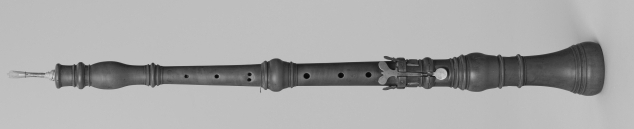
\includegraphics[width=0.9\textwidth]{F4_09somePngOboeBaroqueDennerMIR370}%.png
}
\caption{\label{fig:asIsPng}Some png-picture, directly included }
\end{figure}


% !TEX root = manualLMP.tex
\chapter{Processing of \LaTeX{} Main Files}\label{chap:latexMainConversions}

Given graphics in formats includable in TEX files, 
which may require preprocessing described in 
Chapter~\ref{chap:GraphConversions}, 
this section describes the conversions of latex main files 
into target files in detail. 
The most important target file format is \gls{pdf}. 
Conversion into this format is described in Section~\ref{sec:tex2pdf}. 
Note that \gls{pdf} also occurs as source format 
for included pictures and as intermediate files. 
Specific for \LaTeX{} is the \gls{dvi} format, 
which is supported mainly for historical reasons. 
% FIXME\@: nowhere described. 

Almost independent of the format created, 
Inclusion of bibliographies, indices and glossaries 
requires additional conversions 
done by several auxiliary programs. 
Bibliographies are described in Section~\ref{sec:bibtex}, 
indices in Section~\ref{sec:indices} 
and glossaries in Section~\ref{sec:glossaries}. 
Only at the first sight different 
but behind the scenes quite analogous 
is inclusion of results of code evaluations, 
code in python and other languages described in Section~\ref{sec:pythontex}. 
Here, an auxiliary program essentially invokes the language interpreter. 

Sections~\ref{sec:rerunMakeIndexGlossaries} 
and~\ref{sec:rerunLatex} 
are special in that they describe rerunning auxiliary programs 
and the \LaTeX-to-pdf converter, 
which may be necessary even if certain lists are present 
like table of contents list of figures or list of tables. 

Section~\ref{sec:chkReprod} is special in that it is not related with conversion 
but with checking reproducibility. 

Besides the output formats traditional for \LaTeX, 
\gls{pdf} and \gls{dvi} describing e.g.~books, 
Section~\ref{sec:tex2html} describes creation of 
\gls{html}, Section~\ref{sec:tex2odt} the creation of \gls{odt} and 
Section~\ref{sec:tex2doc} creation of MS Word formats like \gls{docx}. 
Finally, also pure text can be generated 
as described in Section~\ref{sec:tex2txt}. 

\newpage


\section{Transforming \LaTeX{} files into PDF files}\label{sec:tex2pdf}

The next step is to create a PDF file from the TEX files. 
\LaTeX{} distinguishes master TEX files from TEX files intended to be inputted
from elsewhere. 
Not taking comments and that like into account, 
master TEX files roughly have the form 
%
%\lstset{language=tex, basicstyle=\small}
\begin{lstlisting}[language=tex, basicstyle=\small]
\RequirePackage[l2tabu, orthodox]{nag} % optional 
\documentclass{...}

\begin{document}
...
\end{document}
\end{lstlisting}

The core of conversion of a TEX file into a PDF file 
is running a \LaTeX{}-to-pdf converter \texttt{latex2pdf} 
to a master TEX file \texttt{xxx.tex}.
The \LaTeX-to-pdf converter \texttt{latex2pdf} 
is configurable via the parameter \texttt{latex2pdfCommand}. 
Possible values are \lualatex{}, \xelatex{} and \pdflatex, 
where the first is the default for which this software is also tested. 
It is also possible to pass parameters to the \LaTeX{}-to-pdf converter. 
Besides conversion into \gls{pdf} format, 
all converters offer conversion to the older \gls{dvi} format 
via option \texttt{-{}-output-format} as \lualatex{} and \pdflatex, 
or the alternative \gls{xdv} generalizing \gls{dvi} 
as \xelatex{} does with the option \texttt{-{}-no-pdf}. 

In fact, the converter \texttt{latex2pdf} 
does much more than converting TEX files to PDF files. 
Figure~\ref{fig:tex2pdf} shows for \texttt{latex2pdf} set e.g.~to \lualatex{}, 
that besides the PDF file also a LOG file and an AUX file is created. 
The LOG file contains logging information on the run of the conversion 
and the aux-file transports information from one run to the next, 
writing in one run and reading in the next run. 
Thus, conversion goes without it, but it is read if present. 
This is why it is depicted at input side in dashed lines. 

Optionally, an FLS file is created containing paths to the files 
the converted \LaTeX{} file depends on 
and a file with ending \texttt{synctex.gz} 
with information for mapping locations at the created PDF file 
to the according input files. 
This is to support backward search, meaning click on a place in the PDF viewer 
opens an editor in the source file. 

What is in fact in the aux-file depends on the package. 
Among other information, 
also citations and the location of the bibliography file with ending bib 
are present. 
This cannot be used directly in the next \texttt{latex2pdf} run 
to create the bibliography, 
because the entries referenced in the document must be extracted from the bib-file 
and sorted. 
This is done by invoking \texttt{bibtex} between two \texttt{latex2pdf} runs. 
Based on the aux-file, \texttt{bibtex} creates a bbl-file 
containing the bibliography, which is read in the next \texttt{latex2pdf} run. 
For details see Section~\ref{sec:bibtex}. 

Alternatively to \texttt{bibtex} a bibliography can be created 
with the package \pkg{biblatex} in conjunction with the auxiliary program \texttt{biber}. 
Running a \LaTeX-to-pdf converter with package \pkg{biblatex} loaded 
creates a \gls{bcf}-file read by \texttt{biber}. 
This software does not support that option. 
Nevertheless, for sake of completeness we added this data path to Figure~\ref{fig:tex2pdf}. 

If an index is demanded, 
in addition \texttt{latex2pdf} creates a \gls{idx}-file. 
As the citations, it cannot be used directly to create an index in
the next \texttt{latex2pdf} run, 
because the index entries must be collected and sorted before. 
This is done by invoking \texttt{makeindex} 
between the two \texttt{latex2pdf} runs. 
Based on the \gls{idx}-file, \texttt{makeindex} creates a \gls{ind}-file 
containing the index, which is read in the next \texttt{latex2pdf} run. 
For details see Section~\ref{sec:indices}. 

If more than one index is demanded, 
we suggest using \texttt{splitindex} instead of \texttt{makeindex} 
which creates one \gls{ind}-file per index. 

If a glossary is demanded, this can be read off the \gls{aux}-file 
and a \gls{glo}-file containing the index entries 
is created and a file with style information. 
Depending on the configuration, 
this may be a \gls{ist}-file or a \gls{xdy}-file. 
As for the index the \gls{idx}-file, 
the \gls{glo}-file cannot be used directly to create a glossary in
the next \texttt{latex2pdf} run, 
because the glossary entries must be collected and sorted before. 
This is done by invoking \texttt{makeglossaries} 
between the two \texttt{latex2pdf} runs. 
Based on the \gls{glo}-file, \texttt{makeglossaries} creates a \gls{gls}-file 
containing the glossary, which is read in the next \texttt{latex2pdf} run. 
For details see Section~\ref{sec:glossaries}. 

The package \pkg{pythontex} allows including python code or related 
in the \gls{tex}-file and to evaluate it. 
The first \texttt{latex2pdf} run creates a \gls{pytxcode}-file 
which contains essentially the code parts of the \LaTeX-file. 
Invoking \texttt{pythontex} creates by default 
a folder \texttt{pythontex-files-xxx} 
with material where code is already evaluated. 
In the next \texttt{latex2pdf} run, this material is included in the document. 
The \pkg{pythontex} comes with a second command line utility, 
\texttt{depythontex}, eliminating all python code from the original tex-file. 
Optionally, \texttt{latex2pdf} also creates a \gls{depytx}-file 
with all information to replace python code in the original tex-file 
with evaluated material from \texttt{pythontex-files-xxx}. 
Replacement is done by \texttt{depythontex} 
which by default, sends the result to stdout, 
but there is an option to write into another \LaTeX-file. 
Converting this new \LaTeX-file 
yields the same result as converting the original one. 
Depythonization is a feature needed e.g.~for papers 
when the publisher does not accept included code. 
For details see Section~\ref{sec:pythontex}. 

In addition, if
a table of contents, a list of figures, a list of tables 
or a list of listings is required, 
also a toc-file, a lof-file, a lot-file and a lol-file is created,
respectively, 
collecting the according information. 
Also, if hyper-references are built, an \gls{out}-file 
containing bookmarks is created. 
If such a file is present, it is read in and is used
to create a table of contents, a list of figures, of tables and of listings 
or bookmarks in the second run of \texttt{latex2pdf}. 

To summarize, 
if a table of contents, a list of figures, a list of tables, a list of listings or 
a bibliography, an index or a glossary is present, 
or if code must be replaced by their evaluation, 
a second \LaTeX{} run is required to make that material appear in the pdf-output. 

If a table of contents and at the same time 
a bibliography, an index or a glossary is present, 
even two further \LaTeX{} runs are required: 
After the first one, the bibliography, the index or the glossary 
occurs in the PDF file but not yet in the table of contents. 
This happens after the second additional \LaTeX{} run. 
As described in Sections~\ref{sec:rerunMakeIndexGlossaries} and~\ref{sec:rerunLatex}, 
further runs of \texttt{makeindex}, resp,~\texttt{splitindex}, 
\texttt{makeglossaries} 
and of the \LaTeX-processor \texttt{latex2pdf} may be necessary. 

\begin{figure}[htb]
\centering
\IfPackageLoadedTF{tex4ht}{%
should be a picture 
}{
\import{}{F5_01tex2pdf.ptx}
}
\caption{\label{fig:tex2pdf}Conversion of a TEX file into a PDF, DVI, XDV file }
\end{figure}

\section{Bibliographies}\label{sec:bibtex}

In case the \LaTeX{}-to-pdf converter writes bibliographic information, 
into its aux-file, a bibliography must be generated. 
For each occurrence of a \cmd{cite}-command in the TEX file, 
\texttt{latex2pdf} writes an according entry \cmd{citation} into the aux-file. 
Moreover, a \cmd{bibliography}-command in the TEX file 
writes a link to the bib-file containing the bibliography data 
into the aux-file as \cmd{bibdata}. 
Optionally, a \cmd{bibliographystyle}-command in the TEX file 
writes a link to the bibliography style file 
into the aux-file as \cmd{bibstyle}. 

To create a bibliography, 
a \texttt{bibtexCommand} must be run after the \LaTeX{} run. 
The default command is the traditional \texttt{bibtex}, 
but there are more modern alternatives 
like \texttt{bibtexu} and \texttt{bibtex8} supporting utf8 encoding 
and others. 

% mention Biber and biblatex and also mlbibtex 

Essentially, \texttt{bibtex} extracts the citations in the aux-file, 
unifies them, i.e.~a citation is listed once even if it is used more than once, 
retrieves the according entries from the bib-file, sorts these, 
performs formatting and writes all into a bbl-file 
which can be included in the next run of \texttt{latex2pdf}. 

Note that after a \texttt{bibtex}-run, 
two \LaTeX{} runs are required: 
The first one just puts the bibliography found in the bbl-file 
into the PDF file and the labels of the citations into the aux-file 
as \cmd{bibcite}-commands. 
The second run places the labels of the citations found in the aux-file 
at the citations given by \cmd{cite}. 
The package \pkg{tocbibind} described in~\cite{TocBibIndP}, 
then writes the headline of the bibliography into the table of contents.\index{table of contents}
The package \pkg{rerunfilecheck} described in~\cite{RerunFChkP}, 
ensures that \texttt{latex2pdf} is rerun if needed, 
provided loaded with option \texttt{aux}. 


This software presupposes, that \texttt{bibtex} reads the aux-file 
and creates a bbl-file and also an blg-file with logging output 
as illustrated by Figure~\ref{fig:aux2bbl}. 
From the blg-file this software may determine 
whether \texttt{bibtex} emitted an error or warnings. 


\begin{figure}[htb]
\centering
\IfPackageLoadedTF{tex4ht}{%
should be a picture 
}{
\import{}{F5_02aux2bbl.ptx}
}
\caption{\label{fig:aux2bbl}
Conversion of an aux-file into a bbl-file using a bibliography}
\end{figure}

Vital information on \texttt{bibtex} can be found in~\cite{BibPat} 
and in~\cite{BibMar}. 
Also, Chapter 10 in~\cite{Gra} gives vital information on \texttt{bibtex}. 


\section{Indices}\label{sec:indices}

In case the \LaTeX{}-to-pdf converter writes index information, 
into its \gls{idx}-file, at least one index must be generated. 
Since the \gls{idx}-file contains nothing but index information, 
an index is created if and only if the \gls{idx}-file is created. 
% Well, this is not really the truth: it is needed only if ...
Essentially, 
the command \cmd{makeindex}{} tells \texttt{latex2pdf} 
to open the \gls{idx}-file for writing. 
Then for each occurrence of the \cmd{index}-command 
or similar (details see below) in the TEX file, 
an entry is written sequentially to the \gls{idx}-file as 
\cmd{indexentry}{} comprising the keyword given by the \cmd{index}-command 
and the page number where the \cmd{index}-command occured. 
For example \cmd{index\{ant-task\}}{} creates an entry 
%
\begin{lstlisting}[language=TeX]
\indexentry{ant-task|hyperpage}{3}
\end{lstlisting}
%
in \texttt{xxx.idx}. 

Then the \texttt{makeindex}-command is applied to the \gls{idx}-file 
which sorts keywords and for each keyword collects the according page numbers, 
sorts it and and writes the result into a \gls{ind}-file. 
In the next run of \texttt{latex2pdf}, 
the \cmd{prindindex}-command includes the index as a separate section; 
typically at the end of the PDF file. 
The most basic package to provide this command 
is \pkg{makeidx} described in~\cite{MkidxShIdxP}. 
In addition, \pkg{makeidx} provides the command \cmd{see}{} 
which is for cross-reference within an index. 
The package \pkg{tocbibind} described in~\cite{TocBibIndP}, 
then writes the headline of the index into the table of contents.\index{table of contents}
The package \pkg{rerunfilecheck} described in~\cite{RerunFChkP}, 
ensures that \texttt{latex2pdf} is rerun if needed, 
provided loaded with option \texttt{aux}. 

The same document,~\cite{MkidxShIdxP} 
also describes the package \pkg{showidx} 
which prints index entries at the margin of the document. 
This is for debugging only. 
\medskip


The main restriction of the package \pkg{makeidx} is, 
that only a single index can be created. 
The reason is that, \texttt{latex2pdf} creates a single \gls{idx}-file 
and, as illustrated in Figure~\ref{fig:idx2ind}, 
\texttt{makeindex} creates a single ind-file from that, 
representing a single index. 

To overcome this restriction, 
replace package \pkg{makeidx} and \texttt{makeindex} 
with package \pkg{splitidx} and \texttt{splitindex} 
both described in~\cite{SplitidxP}. 

The package \pkg{splitidx} is used 
in conjunction with the program \texttt{splitindex}. 
It must be possible to create a single index 
without using \pkg{splitidx} and \texttt{splitindex}. **** 

Package option \texttt{split} makes \texttt{latex2pdf} 
creating \gls{idx}-files \texttt{xxx-y.idx} directly. 
Here \texttt{y} represents the identifier of an individual index. 
These \gls{idx}-files can be transformed individually with \texttt{makeindex} 
into ind-files as illustrated in Figure~\ref{fig:idx2indMult}. 
Since \texttt{latex2pdf} can keep open only up to 16 output streams, 
not all of which can be used to create a file \texttt{xxx-y.idx}, 
this approach allows a limited number of indices 
and is thus not recommended and not supported. 
Another reason is, that this approach undermines 
the package \pkg{rerunfilecheck} described in~\cite{RerunFChkP}, 
and so it is not guaranteed that \texttt{latex2pdf} is rerun if needed. 
This explains why option \texttt{split} is not allowed. 
% **** check? 

Instead, without option \texttt{split}, 
\texttt{latex2pdf} creates a single \gls{idx}-file. 
The program \texttt{splitindex} splits it up into several \gls{idx}-files 
and applies \texttt{makeindex} to each of them separately 
as illustrated in Figure~\ref{fig:idx2indSplit}. 

For usage of further packages supporting multiple indices 
which are not intended to be used with this software, 
see Chapter~\ref{chap:gaps}. 

This software presupposes, that \texttt{makeindex} converts the \gls{idx}-file 
into an ind-file containing the index 
and creating also an ilg-file with logging output 
as shown in Figure~\ref{fig:idx2ind}. 
From the ilg-file this software may determine 
whether \texttt{makeindex} emitted an error or warnings. 

\begin{figure}[htb]
\centering
\IfPackageLoadedTF{tex4ht}{%
should be a picture 
}{
\import{}{F5_03idx2ind.ptx}
}
\caption{\label{fig:idx2ind}Conversion of an \gls{idx}-file into an ind-file}
\end{figure}

\begin{figure}[htb]
\centering
\IfPackageLoadedTF{tex4ht}{%
should be a picture 
}{
\import{}{F5_04idx2indMult.ptx}
}
\caption{\label{fig:idx2indMult}
Not supported: Conversion of \gls{idx}-files into ind-files}
\end{figure}

\begin{figure}[htb]
\centering
\IfPackageLoadedTF{tex4ht}{%
should be a picture 
}{
\import{}{F5_05idx2indSplit.ptx}
}
\caption{\label{fig:idx2indSplit}Conversion of an \gls{idx}-file into ind-files}
\end{figure}

It is possible to configure the makeindex-command 
and to pass arbitrary options. 
CAUTION\@: For the usual \texttt{makeindex}-command, 
the options \texttt{-o} specifying an output file 
and \texttt{-t} (transcript) specifying the logging file are not allowed, 
because this breaks the expectation to find the sorted index 
in file \texttt{xxx.ind} 
and bypasses the detection of errors and warnings of this software, 
respectively. 
Also specifying a style file via option \texttt{-s} 
is not recommended because this is used to create a glossary 
and so breaks glossary creation 
as described in Section~\ref{sec:glossaries}. 

Information on the makeindex program can be found in~\cite{MkIdxMoe} 
and in~\cite{MkIdxLam}. 
Also, there is a site~\cite{MakeIdxOpts} 
describing all available options for \texttt{makeindex}. 

As indicated above, the program \texttt{splitindex} 
invokes \texttt{makeindex}. 
Its options are described in~\cite{SplitidxP}, Section~3.10. 
Since the long option names are not understood in all environments, 
only the short options are recommended. 

Since \texttt{splitindex} must satisfy the interface 
given by Figure~\ref{fig:idx2indSplit}, 
the option \texttt{--help} and its shortcut \texttt{-h} are not allowed. 
Likewise for option \texttt{--version} and its shortcut \texttt{-V}. 
The option \texttt{--makeindex <makeindex>}, resp.~\texttt{-m <makeindex>}, 
is used with the \texttt{makeindex} command used for single indices. 
Thus, this may not be given explicitly but is specified implicitly. 
Also, the option \texttt{--identify <regex>}, resp.~\texttt{-i <regex>} 
must be set implicitly because it must be the same expression 
as used to ***** 
Then splitindex.tlu is not allowed, 
because this has another expression. 

Only allowable seems \texttt{-V}, the shortcut for \texttt{--verbose}. 

Then comes the name of the index file to be processed 
without suffix. 

The program \texttt{splitindex} invokes \texttt{makeindex}. 
The option option \texttt{--} coming after the filename, 
indicates that all following options are passed to \texttt{makeindex} 



\section{Glossaries}\label{sec:glossaries}

CAUTION\@: The method described here, 
has at least two severe bugs: 
The number of reruns of the \LaTeX-to-pdf converter and also of \texttt{makeglossaries} 
is not guaranteed as a consequence of a bug in \pkg{rerunfilecheck} 
and the fact, that it does not fit current versions of \pkg{makeglossaries}. 
In addition, entries of the glossaries not mentioned directly in the document 
but must be included because they are used in the explanation of entries to be included 
are not treated properly. 

As a consequence, this document, or to be more precise its glossary, 
could not always be reproduced and so the author excluded the glossary until the problem is fixed. 

In addition, it is a conceptual weakness that a glossary data base 
shall be centralized and shall thus not be included in a \LaTeX{} document 
and not even be written in \LaTeX. 
All weaknesses, bugs and conceptual shortcomings are overcome 
by the package \pkg{glossaries-extra} in conjunction with the auxiliary program \texttt{bib2gls} 
which will replace \pkg{glossaries} and \texttt{makeglossaries}. 
For the time being, use glossaries with caution. 
\medskip


Creating glossaries 
requires the package \pkg{glossaries} described in~\cite{GloP}. 
Note that despite the headline of this section, 
and despite \pkg{glossaries} itself supports multiple glossaries, 
this software supports only a single glossary 
and also sorting and unifying is done 
either via \texttt{makeindex} as for indices or via \texttt{xindy}, 
whereas the option to do without external programs 
offered also by package \pkg{glossaries} 
is not supported by this software. 

For generalizations see Chapter~\ref{chap:gaps}. 

As for creating indices there is a \LaTeX-command \cmd{makeindex}, 
to create a glossary there is a \LaTeX-command \cmd{makeglossaries}{}, 
but the latter is not built-in as \cmd{makeindex} 
but provided by the package \pkg{glossaries}. 
If \texttt{xxx.tex} is the \LaTeX{} main file, 
\cmd{makeglossaries}{} opens the glo-file \texttt{xxx.glo} 
containing glossary entries for writing. 
As the built-in command \cmd{index}{} 
writes entries into the \gls{idx}-file defining the index, 
the command \cmd{gls}{} defined by the package \pkg{glossaries} 
writes an entry into the glo-file. 
Note that \texttt{xxx.glo} typically contains entries more than once 
and that the entries are not sorted. 

To perform sorting, formatting and typically also unification, 
the package \pkg{glossaries} allows three mechanisms. 
This software supports two of them: 
via the shell command \texttt{makeindex}, which is also used for indices, 
and via the shell command \texttt{xindy}. 
Using \texttt{makeindex} is the default but can also be activated through 
\cmd{usepackage[makeindex]\{glossaries\}}. 
Using \texttt{xindy} instead of \texttt{makeindex} is triggered through 
\cmd{usepackage[xindy]\{glossaries\}}. 
Accordingly, for option \texttt{makeindex} the aux-file receives lines 
%
\begin{lstlisting}[language=TeX]
\providecommand\@istfilename[1]{}
\@istfilename{manualLMP.ist}
\end{lstlisting}
%
whereas for option \texttt{xindy}, there are lines 
%
\begin{lstlisting}[language=TeX]
\providecommand\@istfilename[1]{}
\@istfilename{manualLMP.xdy}
...
\providecommand\@xdylanguage[2]{}
\@xdylanguage{main}{english}
\providecommand\@gls@codepage[2]{}
\@gls@codepage{main}{}
\end{lstlisting}



This software neither invokes \texttt{makeindex} nor \texttt{xindy} directly. 
Instead, it invokes the shell command \texttt{makeglossaries}
invoked without file ending  
which determines from the aux-file 
whether to invoke \texttt{makeindex} nor \texttt{xindy}. 
Accordingly, it writes the style definition 
by creating an ist-file \texttt{xxx.ist} or an xdy-file \texttt{xxx.xdy} 
if \texttt{makeindex} or \texttt{xindy} is specified as package option, 
respectively. 

Seemingly, \texttt{makeglossaries} relies on the aux-file 
to determine whether to invoke \texttt{makeindex} or \texttt{xindy} 
for sorting and unification. 
Then it invokes the according command and writes a LOG file 
with ending \texttt{glg}, 
redirecting the logging output of \texttt{makeindex} or \texttt{xindy} 
adding own output so that a glg-file may be written, 
even if e.g.~\texttt{makeindex} is invoked and does not. 
In any case, if the glg-file is written, 
\texttt{makeglossaries} writes text matching 
%
\begin{verbatim}
(^\*\*\* unable to execute: )
\end{verbatim}
%
in the glg-file if an error occurs, 
no matter whether \texttt{makeindex} or \texttt{xindy} is invoked. 
Possibly, there are cases where an error causes no glg-file to be written. 
If no error occurs, a glg-file is written 
and if warnings are emitted, 
they either come from \texttt{makeindex} or from \texttt{xindy}. 
Thus warnings may be detected with the patterns 
defined by \texttt{makeindex} and by \texttt{xindy}. 

The style \texttt{list} (which is the default) is set in the form 
%
\begin{lstlisting}[language=TeX]
\usepackage[style=list]{glossaries}
\end{lstlisting}
%
where~\cite{GloP}, Section~15 lists predefined styles. 
So, the style determines the content of the style definition, 
whereas the options \texttt{makeindex} and \texttt{xindy} 
specify the form in which the style is encoded 
and thus the ending of the style file, 
which is either \texttt{ist} or \texttt{xdy}. 

Sorting the glo-file, as said above, 
currently is only supported using the command \texttt{makeglossaries}. 
The allowed options are essentially those 
making sense for \texttt{makeindex} and those making sense for \texttt{xindy}. 
If the shell command \texttt{makeglossaries} 
invokes \texttt{makeindex} of course only the according options 
are passed supplemented by additional options 
\texttt{-s}, \texttt{-t}, \texttt{-o}, to specify the
ist-file, the glg-file (the transcript-file) and the gls-file,
respectively, 
which is the result of sorting, the output file, 
and contains the entries of the glo-file 
just sorted, formatted and unified.
So for a tex main file \texttt{xxx.tex} the program 
\texttt{makeglossaries} invokes
%
\begin{verbatim}
makeindex  -s "xxx.ist" -t "xxx.glg" -o "xxx.gls" "xxx.glo"
\end{verbatim}
%
Accordingly, if the shell command \texttt{makeglossaries} 
invokes \texttt{xindy} of course only the according options 
are passed supplemented by additional options 
\texttt{-M}, \texttt{-t}, \texttt{-o}. 
This is illustrated in Figure~\ref{fig:glo2gls}. 


\begin{figure}[htb]
\centering
\IfPackageLoadedTF{tex4ht}{%
should be a picture 
}{
\import{}{F5_06glo2gls.ptx}
}
\caption{\label{fig:glo2gls}Conversion of a glo-file into a gls-file 
using \texttt{makeglossaries}}
\end{figure}


\section{Including code via \texttt{pythontex}}\label{sec:pythontex}

The package \pkg{pythontex}, described in~\cite{PythonTexP} 
originally allowed including Python code into a latex document. 
Later on, further languages were added, most notably octave or Matlab, 
and the user can easily extended it to further languages 
as sketched in~\cite{PythonTexP}. Section 7. 
Of course, to that end, the interpreter for the desired language must be installed.\index{pythontex}
The meaning of the term ``including'' used above 
ranges from mere listing to pure execution and comprises also inserting results of execution. 
A field of application is also creating figures. 

Note that like the package \pkg{splitindex}, also \pkg{pythonindex} 
comes with an according auxiliary program, 
in this case, besides \texttt{pythontex} also \texttt{depythontex}. 
Consequently,~\cite{PythonTexP} is not only on the package 
but also on the corresponding command line tools. 
Since~\cite{PythonTexP} is quite detailed, 
there is an introduction~\cite{PythonTexQ} and a gallery~\cite{PythonTexG}. 
For background on the intentions of package \pkg{pythontex}, consult~\cite{PythonTexRepr}. 
Information required to integrate pythontex into this software 
partially goes much beyond the official documentation and is collected in~\cite{PyTexInOut}. 
It could also be interesting for the user for debugging. 

Running the \LaTeX-to-pdf converter on a file \texttt{xxx.tex} 
with package \pkg{pythontex} loaded 
yields a file \texttt{xxx.pytxcode} 
and if the package is loaded with option \texttt{depythontex} 
also a file \texttt{xxx.depytx}.
If the file \texttt{xxx.pytxcode} is present, 
this software invokes the command line tool \texttt{pythontex} 
(same name as the according package) 
to \texttt{xxx.pytxcode} (without ending) 
which converts this into a variety of output files, 
which are, without further configuration, 
all in the folder \texttt{pythontex-files-xxx}
as shown in Figure~\ref{fig:py2dir}, 
which is described in more detail in~\cite{PyTexInOut}, Section~3. 
Note that this software uses the wrapper \texttt{pythontexW} 
of \texttt{pythontex} described below, instead of \texttt{pythontex} itself. 
The figure reflects this. 

% TBD: later on, if \texttt{xxx.depytx} after \texttt{pythontex} also \texttt{pythontex} is invoked, 
% creating a tex file without python code. 
% TBD: clarify what if input files or include files are present. 

Running the \LaTeX-to-pdf converter again, 
includes all the output files \texttt{*.stdout} 
in the PDF file or whatever output file created. 

% Note that if depythontex is invoked, it is immaterial whether the subsequent run of LaTeX-to-pdf converter 
% is on the original tex file or on the tex file created by depythontex. 

An important remark is that \lualatex{} is the preferred converter, 
because files \texttt{*.stdout} can impose heavy memory usage 
and currently \lualatex{} is the only converter allocating memory dynamically. 

As one can see, \texttt{pythontex} cooperates with \lualatex{} in a way 
also \texttt{bibtex} or the other auxiliary programs do. 
Although \texttt{pythontex}, at time of this writing in version 0.18, 
is quite mature, it refrains from writing a log file and indicates errors and warnings 
just on standard output or error output. 
This is unlike all the other auxiliary programs in a line with \texttt{pythontex}. 
As a consequence, in particular warnings are difficult to detect 
and cannot be detected in a uniform way. 
Thus, the author wrote a little wrapper, called \texttt{pythontexW} 
%
\begin{verbatim}
  #! /bin/bash
  # bash version >=3.0
  pythontex $@ |& tee ${!#}.plg  
\end{verbatim}
%
and place it where it can be found, e.g.~in the folder of \texttt{pythontex}. 
Note that this is specific for unix-like operating systems 
but can be easily adapted to windows. 
Accordingly, \texttt{depythontex} behaves in a non-standard way: 
Firstly, by default, it does not output a result file but outputs on standard output. 
This can be changed using the option \texttt{--output} or \texttt{-o} for short. 
Also, \texttt{depythontex} changes into interactive mode 
if the output file is already present. 
To avoid this, the option \texttt{--overwrite} is required. 
Overwriting without asking is the standard behavior of all other auxiliary programs. 
As \texttt{pythontex} also \texttt{depythontex} does not write a log file 
but just prints its errors and warnings. 
Thus, the author wrote a little wrapper, called \texttt{depythontexW} 
%
\begin{verbatim}
  #! /bin/bash
  # bash version >=3.0
  depythontex $@ |& tee ${!#}.dplg  
\end{verbatim}
%
and place it where it can be found, e.g.~in the folder of \texttt{depythontex}. 
% TBD: evaluate: maybe it is a better solution to enable this software itself to write the output to a log file. 
\medskip


The package \pkg{pythontex} and the according auxiliary programs are highly configurable, 
more than this software allows. 

In particular, in the \LaTeX{} document, 
the commands \cmd{setpythontexoutputdir} setting the output directory 
and \cmd{setpythontexworkingdir} setting the working directory shall not be used, 
because this software assumes the default, that the working directory is the directory 
containing the \LaTeX{} main file \texttt{xxx.tex}
and the output directory is in the working directory 
and its name is \texttt{pythontex-files-xxx}. 

Further, the package \pkg{pythontex} can be configured with package options when loading the package. 
Since this software is designed for reproducibility, 
most appropriate would be to specify \texttt{runall=true} meaning that even if no python code is modified 
the auxiliary program \texttt{pythontex} executes the python code in the document. 
Also, it is appropriate to specify \texttt{rerun=always}. 
Note that the defaults are \texttt{runall=false} and \texttt{rerun=errors}. 
This behavior makes sense to speed up creation of the document, 
but it differs from the behavior of all other auxiliary programs 
and causes the check for update of output files to fail. 
Moreover, reproducibility is not as easily shown. 

The package documentation~\cite{PythonTexP} suggests, 
that this makes a difference between \texttt{runall=true/false} 
and \texttt{rerun=always/errors} if external sources are modified, 
but as is proved in~\cite{PyTexInOut}, Section 2.1, 
the package translates package option \texttt{runall=true/false} into key value pair \texttt{rerun=always/errors} 
and this is the only information \texttt{pythontex} obtains from the package, 
so there is no difference. 

Also, the auxiliary program \texttt{pythontex} itself can be configured via command line arguments. 
For the package options \texttt{runall} and \texttt{rerun}, 
there are according command line options \texttt{-{}-runall} and \texttt{-{}-rerun} with the same scope. 
Whereas the package merges options \texttt{runall} and \texttt{rerun} silently, 
the auxiliary program \texttt{pythontex} emits an error, if both are combined. 
Essentially one can forget about \texttt{runall} and stick to \texttt{rerun}. 

Strange enough, according to~\cite{PythonTexP}, Section 4.1, package options overwrite command line options. 
This software shall invoke \texttt{pythontex} 
with the option \texttt{-{}-rerun=always} which is thus specified as the default. 
To force unconditional update, this is not sufficient. 
Instead, this software relies on an undocumented feature of auxiliary program \texttt{pythontex} 
which is likely not to change: 
If one of the expected output files is missing, it recreates all output files, independent of command line options and package options. 
Thus, this software deletes one output file if present, before executing \texttt{pythontex}. 

When this software invokes \texttt{pythontex} 
the exit codes may not be changed via \texttt{-{}-error-exit-code}, 
i.e.~if specified then with value \texttt{true}. 
Neither the options \texttt{-{}-interactive}, \texttt{-h}, \texttt{-{}-help} or \texttt{-{}-version} are allowed. 
Currently, this software does not check for options which are not allowed. 
Fortunately, the latter two command line options have no counterpart in the package configuration. 




If we place some code, e.g.~python code as inline code using \cmd{pyc}
%
\begin{lstlisting}[basicstyle=\footnotesize]
  \usepackage[depythontex]{pythontex}
  ...
  \pyc|print(rf'Python inside latex says: "Hello World; 1+1={1+1}"')|
\end{lstlisting}
%
the code is really evaluated and the string result is included at proper place 
as illustrated by the following text which is created by python: 
%
\begin{quote}
  \texttt{\pyc|print(rf'Python inside latex says: "Hello World; 1+1={1+1}"')|}. % chktex 26  chktex 18 chktex 36
\end{quote}
%
Note that the typewriter font is not created by python, 
it is explicitly set to highlight the string created by python, 
but it is python which evaluates the little computation 
and which prints the string. 

Since \texttt{pythontex} is written in python, 
including python code in the \LaTeX{} document 
uses the python interpreter already installed, as a prerequisite of \texttt{pythontex}. 
To use another language, the according interpreter must be installed in addition to python. 



% TBD: create a figure 


% TBD: depythontex


\begin{figure}[!htb]
  \centering
  \IfPackageLoadedTF{tex4ht}{%
  should be a picture 
  }{
  \import{}{F5_07py2dir.ptx}
  }
  \caption{\label{fig:py2dir}Conversion of a \texttt{pytxcode}-file using \texttt{pythontex}}
  \end{figure}


  Figure~\ref{fig:depy2out} shows the files converted by \texttt{depythontex}. 
  As for \texttt{depythontex}, this software uses the wrapper \texttt{depythontexW} 
  of \texttt{depythontex} instead of \texttt{depythontex} itself. 
  This is reflected in the figure. 


  \begin{figure}[!htb]
    \centering
    \IfPackageLoadedTF{tex4ht}{%
    should be a picture 
    }{
    \import{}{F5_08depy2out.ptx}
    }
    \caption{\label{fig:depy2out}Conversion of a \texttt{depytx}-file using \texttt{depythontex}}
    \end{figure}
  
\section{Rerunning the index- and glossary processor}%
\label{sec:rerunMakeIndexGlossaries}

As described in Section~\ref{sec:tex2pdf}, 
running a \LaTeX-to-pdf converter as \texttt{latex2pdf} 
may detect the presence of a bibliography, an index and/or of a glossary 
and writes raw files to describe them. 
After that, an intermediate step is required, 
sorting, unifying and formatting the entries. 
This is always done by an external program. 

In the next step the \LaTeX{} processor must read in the unified entries again. 
Whereas a \LaTeX-run affects neither the bibliography nor python code, 
it may well invalidate the page numbers 
of the entries of the index or of the glossary. 
%Also within a glossary entry, further glossary entries may be included. 
Thus, the sorted index and glossary must be rebuilt 
before the next \LaTeX{} run makes them visible in the PDF file. 

To that end, we use the package \pkg{rerunfilecheck}. 
%
\begin{lstlisting}[language=TeX]
\usepackage[index, glossary]{rerunfilecheck}
\end{lstlisting}
%
must be put before 
%
\begin{lstlisting}[language=TeX]
\usepackage{makeidx}
\makeindex
\usepackage[toc, xindy]{glossaries}
%, xindy or even [xindy={language=english,codepage=utf8}]
% mainly for index and glossaries 
\makeglossaries
\end{lstlisting}
%
in particular before \cmd{makeindex}{} and \cmd{makeglossaries}. 

Note that the package \pkg{hyperref} already loads \pkg{rerunfilecheck} 
but with the wrong options. 
Thus, the above declaration must come before 
%
\begin{lstlisting}[language=TeX]
\usepackage[...]{hyperref}
\end{lstlisting}
%
to avoid error 
%
\begin{verbatim}
Option clash for package rerunfilecheck
\end{verbatim}

Package \pkg{rerunfilecheck} detects almost safely 
changes of the raw index file writing an according message 
into the LOG file. 
That way, it can be determined whether it is necessary 
to rerun \texttt{makeindex} and \texttt{makeglossaries}. 
After that, of course \LaTeX{} must be rerun at least once. 
Note that Section~\ref{sec:rerunLatex} describes 
when to rerun \LaTeX{} without prior running *****

\section{Rerunning the \LaTeX{} processor}\label{sec:rerunLatex}

FIXME\@: a word on change in toc, lof, lot and lol. 

As indicated in the previous sections, 
\texttt{latex2pdf} must be rerun, 
if \texttt{bibtex} or \texttt{makeindex} \texttt{splitindex} 
or \texttt{makeglossaries} 
had been run 
to read in the bibliography created by \texttt{bibtex} 
or the index created by \texttt{makeindex} 
or the glossary created by \texttt{makeglossaries}. 
Likewise, if a toc-file, a lof-file, a lot-file or a lol-file
had been created in the first \texttt{latex2pdf} run, 
another run is needed to read in these files 
to create a table of contents, a list of figures or a list of tables, 
respectively. 
Note that for all these cases, 
the LOG file does not allow to detect that \texttt{latex2pdf} has to be rerun, 
by matching a fixed pattern. 

After the second run of \texttt{latex2pdf}, 
the table of contents,
the list of figures, the list of tables and the list of listings 
are included and a section with the bibliography, 
the index and the glossary are inserted. 
It takes a third run of \texttt{latex2pdf} 
to include the bibliography the index and the glossary 
into the table of contents. 
Also it takes that third run to replace the citations 
with the proper labels given in the bibliography. 

Inserting the table of contents,
the list of figures, the list of tables and the list of listings 
may shift the subsequent text 
which may require another run of \texttt{latex2pdf} 
to get the page numbers right. 
As described in Section~\ref{sec:rerunMakeIndexGlossaries} 
intermediate runs of \texttt{makeindex} and \texttt{makeglossaries} 
may be required 
and these also require another run of \texttt{latex2pdf} 
also to get the page numbers right. 
The package \pkg{rerunfilecheck} allows to detect this need to rerun 
by pattern matching on the LOG file almost for sure: 
Still there is some chance 
that the lengths and the md5-sum of all relevant files 
remain the same, although there is a relevant change. 
In this case, this software fails to update 
triggering another \texttt{latex2pdf} run. 


Note that there are several packages which require additional runs, 
such as the longtable-package, 
which may vary dimensions of tables. 
This software presupposes, that all these reruns 
may be detected by matching a fixed pattern in the LOG file. 
Since packages are frequently changed and new packages are written, 
also the pattern cannot be fixed. 
Thus it is configurable. 
 
Note that, if a package requires running other programs 
between two runs of \texttt{latex2pdf}, 
this would require a change in this software. 

\section{Checking reproducibility}\label{sec:chkReprod}

TBD: this is to be reworked. 

There are use cases, where on the one hand side we want to deliver the sources, 
but it is extremely important that the according artifacts are really reproducible. 
One obvious case is integration test for this software 
by ensuring that each artifact created 
is equivalent with a confirmed version. 
Details are given in Section~\ref{chap:tests}. 



Currently, this is done for PDF files only. 
% TBD: change that 
The problem with PDF files is, that besides visible contents 
they contain also meta-data (see~\cite{pdf17}, Section 14.3), 
which depends on the run of the conversion. 
For example the timestamp of conversion goes into and so do many more aspects. 

There are two strategies to deal with the problem: 
%
\begin{itemize}
  \item 
  Make the build process reproducible. 
  The advantage of this approach is that diffing is quite simple, fast and reproducible: 
  it is byte by byte. 
  This is easily done with a fixed installation but tends to break with update of tools. 
  % TBD: allow own version check. 
  Also, at time of this writing, the different latex engines cannot be treated uniformly. 
  % TBD: a feature request to hyperref is already posted. 
  % let us keep an eye on that. 
  \item 
  Use diff tools implementing a weaker notion of equivalence, 
  in a sense visibility equivalence of some degree. 
\end{itemize}

We support both approaches. 
The first one imposes requirements on the TEX source file. 
It excludes that one displays a creation date changing each run. 
For this manual, we replaced the creation date by a ``version date''. 
A date can be only date of check in of a version control system or that like. 
As an alternative, one could also refrain from using dates altogether. 
In the \texttt{\textbackslash date} command 
one could display also other pieces of information identifying the document. 

But the visible date is not all we have to avoid. 
Listing~\ref{lst:reprPdfEngines} shows how to eliminate metadata 
and to replace with adequate one. 
There is metadata which can be eliminated in a uniform way for all latex engines 
using the package \texttt{hyperref} which the author generally advises. 
Using \texttt{hyperref} with \cmd{hypersetup} 
one can set metadata such as author, title, subject and keyword 
as described in~\cite{HyperTextP}, Section 5.8. 
Here we eliminate creation date and modification date for sake of reproducibility, 
and we also eliminate the producer for security reason. 

Besides the date and time, there is another piece of metadata, the \texttt{trailerid}, 
which is to ensure that each run of a \LaTeX{} to PDF compiler runs 
different PDF files are produced. 
This identifier can only be set in a way specific for the \LaTeX{} compiler. 
Caution: \xelatex{} causes \cmd{ifpdf} to enter always the \texttt{else} branch. 
Note that for \xelatex{} further techniques are required to reach reproducibility. 
% TBD: make this more specific. 
Except for \xelatex, Listing~\ref{lst:reprPdfEngines} provides means to eliminate all information 
making the document reproducible also without \pkg{hyperref}, 
but this applies only to newer versions. 
Besides code the listing provides a lot of documentation. 
In that for \pdflatex{} also the package \pkg{pdfprivacy} described in~\cite{PdfPriv} is mentioned 
as a convenient alternative. 

If a user renounces independence of the engine and sticks to \pdflatex{} only, 
the package \texttt{hyperref} 
could be replaced by specific commands. 
Also, using the package \texttt{iftex} one can detect the used engine 
via the macros \cmd{ifLuaTeX}, \cmd{ifXeTeX} 
and \cmd{ifPDFTeX} as illustrated in Listing~\ref{lst:reprPdfEngines}
and adapt the code to the engine. 

% TBD: clarify: does hyperref replace the engine specific settings? 
% I think no, because of the trailerid, it does not, so iftex is always needed. 
% For pdftex I seem to do twice and once is sufficient. 
% I have the impression some things i do not for reproducibility 
% but I do for security. 
% All in all, we need additional research to write this section in a competent way. 

\lstinputlisting[language={[LaTeX]TeX}, basicstyle=\footnotesize,
firstline=3, 
breaklines,
%float, 
captionpos=b, label={lst:reprPdfEngines},
caption={Create reproducible PDF files for various engines}]%
{./headerSuppressMetaPDF.tex}




Now that we have described how to ensure reproducible PDF artifacts, 
just by designing the TEX source appropriately, 
we have to explain how to check that a newly created artifact 
coincides with a blueprint provided a priori. 
First, note that currently such a check is performed 
only if the result is in PDF format. 
Even then the check is performed only if configured so. 
Then the actual artifacts are compared to predefined artifacts 
using the configured diff-tool. 
If the actual artifacts do not coincide with predefined ones 
according to the chosen diff tool, 
a build exception is thrown as specified in Table~\ref{tab:TLP}. 
The configurations related with diff check are collected in Section~\ref{sec:paramRepro}. 



\section{Creating hypertext}\label{sec:tex2html}

To create HTML and XHTML from TEX files (more precise from \LaTeX{} files), 
a \texttt{tex4htCommand}-command is used 
Together with its parameters, 
it is described in Section!\ref{sec:settingsLatex2Html}. 
This may be \texttt{htlatex}, the default based on \texttt{latex} 
and \texttt{htxelatex} based on \xelatex. 

Figure~\ref{fig:tex2xml} shows the steps \texttt{htlatex} performs: 
From the input \LaTeX{} file \texttt{xxx.tex} 
another \LaTeX{} file \texttt{yyy.tex} is created 
which arises from \texttt{xxx.tex} by adding 
%FIXME\@: maybe instead: \RequirePackage which may be placed before documentclass
\begin{lstlisting}[language=TeX]
\usepackage[...]{tex4ht}. 
\end{lstlisting}
%
Then \texttt{htlatex} runs \texttt{latex} on \texttt{yyy.tex} 
which results in \texttt{yyy.dvi}. 
Note that this is in contrast to \lualatex{} 
which would create some \texttt{yyy.pdf} unless otherwise specified. 

Then comes the converter \pkg{tex4ht} into the game 
which creates several html-files among those also \texttt{xxx.html}. 
The other files, \texttt{yyy.idv} and \texttt{yyy.lg}, 
are further processed by \texttt{t4ht} 
creating the stylesheet \texttt{xxx.css} and graphic files. 
\medskip


Let us make this more precise. 
The output of latex is a standard \gls{dvi}-file 
interleaved with special instructions 
for the post-processor \pkg{tex4ht} to use. 
Note that \pkg{tex4ht} is the name both of the post-processor 
and of the \LaTeX-package. 
The special instructions come from implicit and explicit requests 
made in the source file through commands for TeX4ht. 

The utility \pkg{tex4ht} translates the dvi-code into standard text, 
while obeying the requests it gets from the special instructions. 
The special instructions may request the creation of files, 
insertion of html code, filtering of pictures, and so forth. 
In the extreme case that the source code contains no commands of TeX4ht, 
\pkg{tex4ht} gets pure dvi-code and it outputs (almost) plain text 
with no hypertext elements in it.

The special (\cmd{special}) 
instructions seeded in the dvi-code 
are not understood by dvi processors other than those of TeX4ht.

\texttt{t4ht}
This is an interpreter 
for executing the requests made in the \texttt{xxx.lg} script.

\texttt{xxx.idv}
This is a dvi-file extracted from \texttt{xxx.dvi}, 
and it contains the pictures needed in the html files.

\texttt{xxx.lg}
This is a log file listing the pictures of \texttt{xxx.idv}, 
the \gls{png} files that should be created, CSS information, 
and user directives introduced 
through the ``\cmd{Needs\{\ldots\}}'' command.

\raggedbottom{}


\begin{figure}[!htb]
\centering
\IfPackageLoadedTF{tex4ht}{%
should be a picture 
}{
\import{}{F5_09tex2xml.ptx}
}
\caption{\label{fig:tex2xml}Conversion of a TEX file into an xml-file}
\end{figure}

% LTeX: enabled=false
\begin{Verbatim}[fontsize=\tiny]
(/usr/local/texlive/2014/texmf-dist/tex/generic/tex4ht/tex4ht.4ht
version 2009-01-07-07:11
--------------------------------------
Note --- for additional information, use the command line option `info'
--------------------------------------

(/usr/local/texlive/2014/texmf-dist/tex/generic/tex4ht/html4.4ht

Note: to remove the <?xml version=...?> processing instruction 
use the command line option `no-VERSION'

Note: to remove the DOCTYPE declaration 
use the command line option `no-DOCTYPE'
)

--------------------------------------
Note: for marking of the base font, use the command line option `fonts+'
Note: for non active _, use the command line option `no_'
Note: for _ of catcode 13, use the command line option `_13'
Note: for non active ^, use the command line option `no^'
Note: for ^ of catcode 13, use the command line option `^13'
--------------------------------------

(/usr/local/texlive/2014/texmf-dist/tex/generic/tex4ht/html4.4ht
--------------------------------------
Note: For section filenames that reflect on their titles 
use the command line option `sec-filename'

Note: for alternative charset, use the command line option `charset=...'

Note: to ignore CSS font decoration, use the `NoFonts' command line option

Note: for jpg bitmaps of pictures, 
use the `jpg' command line option. 
(Character bitmaps are controled only by `g' 
records of tex4ht.env and `-g' switches of tex4ht.c) 

Note: for gif bitmaps of pictures, use the `gif' command line option. 
(Character bitmaps are controled only by `g' 
records of tex4ht.env and `-g' switches of tex4ht.c) 

Note: for content and toc in 2 frames, 
use the command line option `frames'

Note: for content, toc, and footnotes in 3 frames, 
use the command line option `frames-fn'

Note --- for file extension name xht, use the command line option `xht'
--------------------------------------
TeX4ht package options: xhtml,uni-html4,2,pic-tabular,html
--------------------------------------
Note: to ignore CSS code, use the command line option `-css

Note: for inline CSS code, use the command line option `css-in'

Note: for pop ups on mouse over, use the command line option `mouseover'

Note: for addressing images in a subdirectory, 
use the command line option `imgdir:.../'
)

Note --- for back links to toc, use the command line option `sections+'

Note --- for linear crosslinks of pages, use the command line option `next'

(/usr/local/texlive/2014/texmf-dist/tex/generic/tex4ht/latex.4ht
version 2009-05-21-09:32
--------------------------------------
Note --- for links into captions, instead of float heads, use the command l
ine option `refcaption'
--------------------------------------

(/usr/local/texlive/2014/texmf-dist/tex/generic/tex4ht/html4.4ht
--------------------------------------
Note --- For mini tocs immediately aftter the header 
use the command line option `minitoc<'

Note --- for enumerated list elements with valued data, 
use the command line option `enumerate+'

Note --- for enumerated list elements li's with value attributes, use the c
ommand line option `enumerate-'

Note --- for CSS2 code, use the command line option `css2'

Note --- for bitmap fbox'es, use the command line option `pic-fbox'

Note --- for bitmap framebox'es, use the command line option `pic-framebox'

Note --- for inline footnotes use command line option `fn-in'

Note --- for tracing of latex font commands, 
use the command line option `fonts'
--------------------------------------
--------------------------------------
Note --- for width specifications of tabular p entries, 
use the `p-width' command line option 
or a configuration similar to 
\Configure{HColWidth}{\HCode{style="width:\HColWidth"}}
--------------------------------------
)
(/usr/local/texlive/2014/texmf-dist/tex/generic/tex4ht/html4-math.4ht
version 2009-05-18-23:01
--------------------------------------
Note --- for pictorial eqnarray, use the command line option `pic-eqnarray'

Note --- for pictorial array, use the command line option `pic-array'

Note --- for pictorial $...$ environments, 
use the command line option `pic-m' (not recommended!!)

Note --- for pictorial $...$ and $$...$$ environments with latex alt, 
use the command line option `pic-m+' (not safe!!)

Note --- for pictorial array, use the command line option `pic-array'
)
(/usr/local/texlive/2014/texmf-dist/tex/generic/tex4ht/unicode.4ht
version 2010-12-18-17:40
)
(/usr/local/texlive/2014/texmf-dist/tex/generic/tex4ht/html4-uni.4ht))


(/usr/local/texlive/2014/texmf-dist/tex/generic/tex4ht/html4.4ht
--------------------------------------
Note --- for tocs without * entries, use command line option `notoc*'

Note --- for tocs without * entries, use command line option `notoc*'

Note --- to eliminate mini tables of contents, 
use the command line option `nominitoc'

Note --- for frames-like object-based table of contents, 
use the command line option `obj-toc'

Note --- for files named derived from section titles, 
use the command line option `sec-filename'

Note --- for i-columns index, 
use the command line option `index=i' (e.g., index=2)
--------------------------------------
)

(/usr/local/texlive/2014/texmf-dist/tex/generic/tex4ht/html4.4ht

Note --- if included graphics are of degraded quality, 
try the command line options `graphics-num' or `graphics-'. 
The `num' should provide the density of pixels in the bitmaps (e.g., 110). 

Note --- for key dimensions try the option `Gin-dim'; 
for key dimensions when bounding box is unavailable 
try `Gin-dim+'; neither is recommended
)

(/usr/local/texlive/2014/texmf-dist/tex/generic/tex4ht/html4.4ht
Note --- for URL encoding within href use the command line option `url-enc'
)

(/usr/local/texlive/2014/texmf-dist/tex/generic/tex4ht/html4.4ht

Note --- for pictorial longtable, 
use the command line option `pic-longtable'
)

(/usr/local/texlive/2014/texmf-dist/tex/generic/tex4ht/html4.4ht

Note --- to ensure proper alignments use fixed size fonts (see listings.dtx
)
)
\end{Verbatim}
% LTeX: enabled=true

\pkg{tex4ht} yields 

\begin{Verbatim}[fontsize=\scriptsize]
----------------------------
tex4ht.c (2012-07-25-19:36 kpathsea)
tex4ht 
--- error --- improper command line
tex4ht [-f<path-separator-ch>]in-file[.dvi]
   [-.<ext>]            replacement to default file extension name .dvi
   [-c<tag name>]       choose named segment in env file
   [-e<env-file>]
   [-f<path-separator-ch>]        remove path from the file name
   [-F<ch-code>]        replacement for missing font characters; 0--255; default 0
   [-g<bitmap-file-ext>]
   [-h(e|f|F|g|s|v|V)]  trace: e-errors/warnings, f-htf, F-htf search
                            g-groups, s-specials, v-env, V-env search
   [-i<htf-font-dir>]
   [-l<bookkeeping-file>]
   [-P(*|<filter>)]     permission for system calls: *-always, filter
   [-S<image-script>]
   [-s<css-file-ext>]   default: -s4cs; multiple entries allowed
   [-t<tfm-font-dir>]
   [-u10]               base 10 for unicode characters
   [-utf8]              utf-8 encoding for unicode characters
   [-v<idv version>]    replacement for the given dvi version
   [-xs]           ms-dos file names for automatically generated gifs
\end{Verbatim}


\texttt{t4ht} yields 

\begin{Verbatim}[fontsize=\footnotesize]
--------------------------------------------------------------------
t4ht [-f<dir char>]filename ...
  -b     ignore -d -m -M for bitmaps
  -c...  choose named segment in env file
  -d...  directory for output files       (default:  current)
  -e...  location of tex4ht.env
  -i     debugging info
  -g     ignore errors in system calls
  -m...  chmod ... of new output files (reused bitmaps excluded)
  -p     don't convert pictures           (default:  convert)
  -r     replace bitmaps of all glyphs    (default:  reuse old ones)
  -M...  chmod ... of all output files
  -Q     quit, if tex4ht.c had problems
  -S...  permission for system calls: *-always, filter
  -X...  content for field %%3 in X scripts
  -....  content for field %%2 in . scripts

Example: 
   t4ht name -d/WWW/temp/ -etex4ht-32.env -m644
--------------------------------------------------------------------
\end{Verbatim}

\flushbottom

\section{Creating odt-files}\label{sec:tex2odt}

\section{Creating MS word files}\label{sec:tex2doc}

The best way to convert \LaTeX{} files into MS word files is via ODT files. 
Conversion from \LaTeX{} to odt 
is already described in Section~\ref{sec:tex2odt}. 
The last step can be done by \texttt{odt2doc} which can create both 
doc-format and docx-format and many others 
which is illustrated in Figure~\ref{fig:tex2doc}. 


\begin{figure}[htb]
\centering
\IfPackageLoadedTF{tex4ht}{%
should be a picture 
}{
\import{}{F5_10tex2doc.ptx}
}
\caption{\label{fig:tex2doc}Conversion of a TEX file into a docx-file}
\end{figure}



\section{Creating plain text files}\label{sec:tex2txt}

Why should one create plain text from \LaTeX{} files? 
Maybe this is the minimal format the receiver can work with. 
Another common application is word-count, 
in particular if writing a paper for a journal. 

Plain text files can be created from \LaTeX{} files 
just by stripping off the tex-commands. 
The disadvantage is, 
that references, bibliography, index, glossary, 
table of contents, list of figures, list of tables, \dots 
and symbols get lost. 
Thus, the first step we take is complete creation of a PDF file 
except display of warnings like bad boxes 
as described in Section~\ref{sec:tex2pdf}. 
This creates an appropriate pdf-file, 
with correct numbering and links, 
possibly with overfull boxes and that like. 
As a final step, we convert the pdf-file into a text file 
using, as a default \texttt{pdftotext} with ending \texttt{txt}. 
Figure~\ref{fig:tex2txt} illustrates the translation process. 

\begin{figure}[htb]
\centering
\IfPackageLoadedTF{tex4ht}{%
should be a picture 
}{
\import{}{F5_11tex2txt.ptx}
}
\caption{\label{fig:tex2txt}Conversion of a TEX file into a txt-file}
\end{figure}

Note that \texttt{pdftotext} produces a text file with page numbers 
and signifies the end of a page 
(to see how, just have a look at the end of the file), 
so that one can identify page numbers as such. 
Thus references, index, glossary, table of contents and that like 
referring to page numbers carry valuable information. 
Also symbols available in utf8 encoding are preserved. 
In contrast, heavily stacked formulae become unreadable, 
because \texttt{pdftotext} displays them line by line 
and drops fraction bars completely. 
Also, formulae with complex subformulae in a root operator  
become unreadable because the root operator becomes just a root symbol. 
Likewise for integrals and that like. 

Aspects of figures kept are the captions of course but also the \LaTeX-texts. 
This is displayed line-wise. 
What gets lost is the postscript/pdf-parts, i.e.~the plain graphics. 

\raggedbottom{}


% !TEX root = manualLMP.tex

\chapter{Parameters resp. Settings}\label{chap:settings}

This section describes the parameters 
of both the ant-task and the maven-plugin. 
As this software mainly acts by invoking converters, 
most parameters refer to commands and options for invocations, 
but there are general aspects, treated in Section~\ref{sec:genOnSettings}, 
but there are also parameters which cannot be associated to an individual converter. 
These are collected in Section~\ref{sec:settingsGen}. 
All the other sections refer to one or more converters. 

The parameters are listed 
in Tables~\ref{tab:paramGen}~through~\ref{tab:paramExt} 
with names, default values and short explanations. 
Note that neither of the parameters is mandatory, 
as there are always valid default values. 

Each of the tables is described in a separate section. 
Table~\ref{tab:paramGen} 
shows parameter controlling the general conversion process 
described in detail in Section~\ref{sec:settingsGen}. 
These are directories with names \texttt{xxxDirectory} 
and further parameters not following a naming convention. 
The other tables show parameters after a certain naming scheme: 
Command names have the form \texttt{xxxCommand} 
and the parameter with the according options have the form \texttt{xxxOptions}. 
Here \texttt{xxx} represents a certain converter. 
This is one of 
%
\begin{itemize}
\item[fig2dev]
The converter of fig-files into mixed latex- and PDF-files. 
\item[gnuplot]
The converter of gnuplot-files into mixed latex- and PDF-files. 
\item[metapost]
The converter of MetaPost-files into mixed latex- and PDF-files.
\item[latex2pdf]
The converter of latex-files into PDF-files. 
\item[bibtex]
The creator of a bibliography from an aux-file.
\item[makeindex]
The makeindex utility creating an index. 
\item[makeglossaries]
The makeglossaries utility creating a glossary. 
\item[pythontex]
The utility to invoke python and other languages from within \LaTeX{} 
and to replace the code by its results dynamically. 
\item[depythontex]
The utility to replace code finally after a run of \texttt{pythontex}. 
\item[tex4ht]
The converter of latex into HTML and also into ODT, 
depending on the parameters. 
\item[latex2rtf]
The converter of latex-files into RTF-files. 
\item[odt2doc]
The converter of ODT-files into doc(x)-files. % chktex 36
\item[pdf2txt]
The converter of PDF-files into TXT-files. 
\item[chktex]
A code-checker converting in a sense a latex main file into a log-file 
containing errors, warnings and further messages. 
\end{itemize}

It is a little more complicated 
with the parameters in Section~\ref{sec:settingsLatex2Html}. 

There are some parameters of the form \texttt{patternXxxYyy}, 
referring to a pattern in the log-file of the converter \texttt{Xxx} 
indicating an event \texttt{Yyy} which is one of the following: 
%
\begin{itemize}
\item[ReRun]
indicates that \texttt{Xxx} needs to be rerun.
\item[Err]
indicates that \texttt{Xxx} had an error. 
\item[Warn]
indicates that \texttt{Xxx} had a warning. 
\end{itemize}

Essentially, there are two kinds of parameters: 
Most are just passed to the converters invoked by this software. 
The parameters of this software 
are so that the choice of the converter, i.e.~the name of the application 
can be configured, 
and also each converter can be almost freely configured. 

Parameters not passed to an application, 
are either really crucial 
or are included to allow also development of latex files. 

\section{Generalities on Parameters}\label{sec:genOnSettings}

As pointed out in the introduction of this chapter, 
this software acts mainly by invoking various converters. 
The converters are grouped in so-called \emph{categories}. 
The converters of a category have the same (file-)interface, %chktex 36
means read and write the same files and, 
mostly but not strictly necessarily, have the same options. 
For each category there is an option \texttt{xxxCommand}, 
where \texttt{xxx} is the name of the category in lowercase letters\footnote%
{In fact there are exceptions to this rule: E.g.~for category \texttt{LaTeX} 
the command is called \texttt{latex2pdf} referring to the common output format \gls{pdf}, 
although also \gls{dvi} and \gls{xdv} are possible}. 
The value of the option is the command to invoke the converter of the category. 
Also, there is a default converter in each category, 
and sometimes there is just a single converter possible. 
For example, \lualatex{} is the default converter in the category \texttt{latex}. 

This software knows about converters and registers the ones approved for this software. 
Among the advantages are, that it is ensured that the converter is really in that category 
and that this software checks whether a converter used is in the right category, 
and it checks whether it is installed in an approved version. 
On the other hand, there are cases, where the user needs to invoke a custom converter. 
In this case, the command name shall be given in the form 
%
\begin{verbatim}
  <categoryCommand>commandName:category</categoryCommand>
\end{verbatim}
%
to make sure, that the user is really aware that the converter (s)he uses % chktex 36
is in the correct category, i.e.~has the required interface. 
Since neither of the registered converters has a \texttt{:} in its name, 
This form is identified by the occurrence of a colon. 
Since the categories neither have colons in their names, 
separation of command name and category is by the last colon occurring. 
That way, command names may contain colons also. 

For most categories of converters, in fact at the time of this writing with a single exception, 
one can specify command line options, specified in the form 
%
\begin{verbatim}
  <categoryOptions></categoryOptions>
\end{verbatim}
%
In fact, only for \texttt{diffPdfCommand} there is no option at all, 
and for some converters with more complex options, the options are split over more than one setting, 
e.g.~for converter category \texttt{fig2dev} converting \gls{fig}-files, 
there are general settings given by \texttt{fig2devGenOptions}
and settings specific for the output language: 
\LaTeX{} (\texttt{fig2devPtxOptions}) and \gls{eps} (\texttt{fig2devPdfEpsOptions}. 
In any case, options are trimmed, i.e.~leading and trailing white spaces are removed 
before being processed. 
There are cases, where the options as given are not directly passed to the converter 
but is further processed. 
In this case, the processing is documented. 

% log, patterns warn, err. 




\section{General Parameters}\label{sec:settingsGen}

This section describes the parameters of Table~\ref{tab:paramGen}. 
%TODO\@: do this. 

\begin{longtable}{|ll|}
\toprule
Parameter        & Default  \\
\multicolumn2{|l|}{Explanation }  \\
\midrule
\midrule
\endfirsthead%
\bottomrule
\caption{\label{tab:paramGen} General parameters}
\endlastfoot%
\texttt{versionsWarnOnly}  & \texttt {false}  \\
\multicolumn2{|l|}{
\begin{minipage}{0.95\linewidth}
Indicates whether the \texttt{VersionMojo} displays warnings only 
or also creates pieces of info. 
Info refers to the version of this plugin and also on its git commit, 
but also on the versions of the converters found 
and lists the converters excluded, i.e.\@ those not used
and thus not tested on version.

Warnings are emitted e.g. 
if the version of a converter does not fit the expectations,
the version of a converter could not be retrieved,
e.g.\@ because it is not installed 
or if the converter specified is unknown altogether. 
This defaults to \texttt{false} displaying also info.

The latter is appropriate for using in command line 
\texttt{mvn latex:vrs}, whereas in builds by default 
the pom overwrites this to have output only 
in case something goes wrong.
\end{minipage}
} \\
\texttt{texSrcDirectory}  & \texttt {src/site/tex}  \\
\multicolumn2{|l|}{
\begin{minipage}{0.95\linewidth}
The latex source directory as a string 
relative to \texttt{\$baseDirectory}, 
containing \texttt{\$texSrcProcDirectory}. 
This directory determines also the subdirectory of 
\texttt{\$outputDirectory} to lay down the generated artifacts. 
The default value is ``\texttt{src/site/tex}'' on Unix systems. 
\end{minipage}
} \\
\texttt{texSrcProcDirectory}  & \texttt {.}  \\
\multicolumn2{|l|}{
\begin{minipage}{0.95\linewidth}
The latex source processing directory as a string 
relative to \texttt{\$texSrcDirectory}
containing all tex main documents 
and the graphic files to be processed 
and also to be cleaned. 
Whether this is done recursively in sub-folders 
is specified by \texttt{\$readTexSrcProcDirRec}. 
The default value is ``\texttt{.}''. 
\end{minipage}
} \\
\texttt{readTexSrcProcDirRec}  & \texttt{true}  \\
\multicolumn2{|l|}{
\begin{minipage}{0.95\linewidth}
Whether the tex source directory \texttt{\$texSrcProcDirectory} 
shall be read recursively for creation of graphic files, 
i.e.~including the sub-directories recursively. 
This is set to \texttt{false} only during development of documentation. 
%The default value is 'true'.
\end{minipage}
} \\
\texttt{outputDirectory}  & \texttt{.}             \\
\multicolumn2{|l|}{
\begin{minipage}{0.95\linewidth}
The generated artifacts will be copied to \texttt{outputDirectory}
relative to \texttt{\$targetSiteDirectory} 
which is by default '\texttt{\$targetDirectory/site}' on Unix systems. 
%The default value is '\texttt{.}'.  
\end{minipage}
} \\
\texttt{targets}          & \texttt{pdf, html}     \\
\multicolumn2{|l|}{
\begin{minipage}{0.95\linewidth}
A comma separated list of targets to be stored in \texttt{\$targetSet}. 
Allowed values are \texttt{pdf}, \texttt{dvi}, \texttt{html}, 
\texttt{txt}, \texttt{odt} and \texttt{docx}. 
Note that if \texttt{\$latex2pdfCommand} is set to \xelatex, 
the format \texttt{dvi} and what is based on it are not supported. 
%The default value is '\texttt{pdf, html}'. 
\end{minipage}
} \\
\texttt{convertersExcluded}          & empty     \\
\multicolumn2{|l|}{
\begin{minipage}{0.95\linewidth}
A comma separated list of excluded {Converter}s 
given by their command. 
Excluded converters need not be installed, but their names must be known. 
They don't show up in the version check of target \texttt{vrs} 
and of course they are not allowed to be used. 
% By default, this list is empty. 
\end{minipage}
} \\
\texttt{patternLatexMainFile} & see Section~\ref{subsec:patternLatexMainFile}\\
\multicolumn2{|l|}{
\begin{minipage}{0.95\linewidth}
The pattern to be applied to the contents of tex-files 
which identifies a \LaTeX{} main file. 
Here we assume that the latex main file should contain 
the declaration ``\cmd{documentclass}'' 
or the old-fashioned ``\cmd{documentstyle}'' 
preceded by a few constructs. 
Strictly speaking, this is not necessary. 
For a more thorough discussion, 
and for an alternative approach, consult the manual. 

The default value is chosen to match quite exactly 
the latex main files, no more no less. 
Since the pattern is chosen 
according to documentation collected from the internet, 
one can never be sure whether the pattern is perfect. 

If the current default value is not appropriate, 
please overwrite it in the configuration 
and notify the developer of this plugin of the deficiency. 
\end{minipage}
} \\
\texttt{mainFilesIncluded}          &  empty string        \\
\multicolumn2{|l|}{
\begin{minipage}{0.95\linewidth}
  The list of names of latex main files 
  without extension \texttt{.tex} separated by whitespace 
  which shall be included for creating targets, 
  except if this is empty in which cases all are included. 
  It is assumed that the names of the latex main files 
  do not contain whitespace. 
  Note that leading and trailing whitespace are trimmed. 
  Currently, names of latex main files 
  should better have pairwise different names, 
  even if in different directories. 
  The empty string is the default, i.e.\@ including all. 
  See parameter \texttt{mainFilesExcluded}. 
\end{minipage}
} \\
\texttt{mainFilesExcluded}          &  empty string        \\
\multicolumn2{|l|}{
\begin{minipage}{0.95\linewidth}
  The list of names of latex main files 
  without extension \texttt{.tex} 
  separated by whitespace 
  which shall be excluded for creating targets. 
  It is assumed that the names of the latex main files 
  do not contain whitespace. 
  Note that leading and trailing whitespace are trimmed. 
  Currently, names of latex main files 
  should better have pairwise different names, 
  even if in different directories. 
  Together with \texttt{mainFilesExcluded}, 
  this is used for document development 
  to build the PDF-files of a subset of documents 
  and e.g.\@ because for a site one needs all documents, 
  but with the software only the manual is shipped. 
  The empty string is the default, i.e.\@ excluding no file. 
  See parameter \texttt{mainFilesIncluded}. 
\end{minipage}
} \\
\texttt{texPath}          &  empty string        \\
\multicolumn2{|l|}{
\begin{minipage}{0.95\linewidth}
Path to the TeX scripts or null. 
In the latter case, the scripts must be on the system path. 
Note that in the pom, \texttt{$<$texPath/$>$} 
and even \texttt{$<$texPath$>$\ \ \ \ $<$/texPath$>$} represent the null-File. 
The default value is null.
\end{minipage}
} \\
\texttt{cleanUp}             & \texttt{true}             \\
\multicolumn2{|l|}{
\begin{minipage}{0.95\linewidth}
Clean up the working directory in the end? 
May be used for debugging when setting \texttt{false}. 
%The default value is '\texttt{true}'. 
\end{minipage}
} \\
\texttt{patternCreatedFromLatexMain} & 
see Section~\ref{subsec:patternCreatedFromLatexMain} \\
\multicolumn2{|l|}{
\begin{minipage}{0.95\linewidth}
This pattern is applied to file names 
and matching shall accept all the files 
which were created from a latex main file `\texttt{xxx.tex}'. 
It is neither applied to directories 
nor to `\texttt{xxx.tex}' itself. 
It shall comprise neither graphic files to be processed 
nor files created from those graphic files. 

This pattern is applied 
in the course of processing graphic files 
to decide which graphic files should be processed 
(those rejected by this pattern) 
and to log warnings if there is a risk, 
that graphic files to be processed 
are skipped or that processing a latex main file overwrites 
the result of graphic preprocessing. 

When clearing the tex source processing directory 
\texttt{\$texSrcProcDirectory}, 
i.e.~all generated files should be removed, 
first those created from latex main files. 
As an approximation, 
those are removed which match this pattern. 

The sequence `\texttt{T\$T}' 
is replaced by the prefix `\texttt{xxx}'. 
The sequence `\texttt{T\$T}' must always be replaced: 
The symbol `\texttt{\$}' occurs as end-sign as `\texttt{)\$}' % chktex 9
or as literal symbol as `\texttt{\$}'. 
Thus, `\texttt{T\$T}' is no regular occurrence 
and must always be replaced with `\texttt{xxx}'. 
		 
Spaces and newlines are removed 
from that pattern before matching. 

This pattern may never be ensured to be complete, 
because any package 
may create files with names matching its own patterns 
and so any new package may break completeness. 
Nevertheless, the default value aims completeness 
while be tight enough not to match names of files not created. 

If the current default value is not appropriate, 
please overwrite it in the configuration 
and notify the developer of this plugin of the deficiency. 
\end{minipage}
} \\ % chktex 9 chktex 10 (bug) 
\end{longtable}


\subsection{The parameter \texttt{patternLatexMainFile}}%
\label{subsec:patternLatexMainFile}

The default pattern for identifying a \LaTeX{} main file 
is given by Listing~\ref{lst:patternLatexMainFile}.

\lstinputlisting[language=XML, basicstyle=\footnotesize,
firstline=141, lastline=148,
breaklines,
%float,
captionpos=b, label={lst:patternLatexMainFile},
caption={The default pattern of the latex main file in a form as in a pom configuration}]
{../../main/resources/rawPoms/pom4pdf.xml}% chktex 11 

% \begin{Verbatim}[fontsize=\footnotesize]
% \A(\\RequirePackage\s*(\[(\s|\w|,)*\])?\s*\{\w+\}\s*(\[(\d|\.)+\])?|
% \\PassOptionsToPackage\s*\{\w+\}\s*\{\w+\}|
% %.*$|
% \\input\{[^{}]*\}|
% \s*)*
% \\(documentstyle|documentclass)
% \end{Verbatim}

This means that the latex main file is the one 
containing \cmd{documentclass}{} for modern classes 
and \cmd{documentstyle}{} for old-fashioned ones. 
This may be preceded only by 
%
\begin{itemize}
\item
the command \cmd{RequirePackage}, 
\item
the command \cmd{PassOptionsToPackage}, 
\item
by comment lines, 
\item
by \cmd{input}, and 
\item
by space. 
\end{itemize}
%
Note that \cmd{A}{} represents the beginning of the stream. 

Strictly speaking, also \cmd{(re)newcommands} % chktex 36
and other constructs are possible but not allowed here. 
Strictly speaking also \cmd{documentclass}{} is not required, 
it could be hidden in some \cmd{input}-file. 
If we stick to the wise convention to open and close the same environment 
in the same file and to have \cmd{documentclass}, 
\cmd{begin\{document\}}{} and \cmd{end\{document\}}{} 
in the same file also, 
then a latex main file without \cmd{documentclass}{} 
cannot contain very much material. 

So we ask the user to have \cmd{documentclass}{} 
declared in the latex main file. 

For users of Emacs with package auctex, there is a valuable alternative: 

Latex main files are marked with an end section as this file: 
%
\begin{Verbatim}[fontsize=\footnotesize]
%%% Local Variables: 
%%% mode: latex
%%% TeX-command-extra-options: "-recorder -shell-escape" 
%%% TeX-master: t
%%% End: 
\end{Verbatim}
% 
The vital line in this context is \texttt{\%\%\% TeX-master: t}. 
In contrast to this, a non-master file 
either has no end-section at all or has an end section 
declaring the according master file (if it is unique) 
explicitly as the following one from \texttt{header.tex}: 
%
\begin{verbatim}
%%% Local Variables:
%%% mode: latex
%%% TeX-master: "manualLMP"
%%% End:
\end{verbatim}

So a pattern for latex main files could also be 
%
\begin{verbatim}
^%%% Local Variables: $
^%%% TeX-master: t$
^%%% End: ^
\s*
\end{verbatim}

For users of visual code/latex workshop, there is another alternative: 
Absence of first line \texttt{\%~!TEX root}. 

Also, if one wants to have a solution not relying on a tool-chain 
not even on \LaTeX{} tools, 
One could use a convention, e.g.~marking main files with first line \texttt{\% MAIN FILE}, 
which makes parsing quite fast. 


\subsection{The parameter \texttt{patternCreatedFromLatexMain}}%
\label{subsec:patternCreatedFromLatexMain}

The files created from a latex main file 
depend strongly on the compiler options 
and on packages used in the latex main file 
and in the TEX-files inputted. 
The default value 
`\texttt{\^{}T\$T\textbackslash.$[$\^{}.$]*$}' 
is appropriate for most parameters and packages: 
most packages create files with names only 
which coincide with the name of the latex main file, except the suffix. 
This is all sufficient even for programs doing post-processing 
such as \texttt{bibtex}, \texttt{makeindex}, \texttt{xindy} and 
\texttt{makeglossaries}. 
The only exception is \texttt{splitindex} 
which requires in addition 
`\texttt{\^{}T\$T\textbackslash-.+\.(idx|ind|ilg)}'. 

Package `\pkg{srcltx}' requires in addition 
`\texttt{\^{}T\$T\textbackslash.synctex\textbackslash.gz}' 
and finally package `\pkg{tex4ht}' is for all the rest. 
The pattern is designed 
to match quite exactly the created files, 
not much more and at any case not less. 
In particular, it has to comprise the files matching pattern 
\texttt{\$patternT4htOutputFiles}. 
Nevertheless, since any new package may break the pattern, 
and not every package is well documented, 
this pattern cannot be guaranteed to be final. 

If the current default value is not appropriate, 
please overwrite it in the configuration 
and notify the developer of this plugin of the deficiency. 

The default value for this pattern is currently: 
%
\begin{verbatim}
^(
T$T             (\.([^.]*|synctex\.gz|out\.ps)|
   (-|ch|se|su|ap|li)?\d+\.x?html?|
             \d+x\.x?bb|
             \d+x?\.png|
             -\d+\.svg)|
zzT$T\.e?ps|
(cmsy)\d+(-c)?-\d+c?\.png|
(pdf)?latex\d+\.fls)$
\end{verbatim}


\section{Parameters for graphical preprocessing}\label{sec:settingsGraph}

This section describes the parameters for graphical preprocessing 
given in Table~\ref{tab:paramGraphics}. 

TODO\@: do this. 


\begin{longtable}{|ll|}
\toprule
Parameter        & Default  \\
\multicolumn2{|l|}{Explanation }  \\
\midrule
\midrule
\endfirsthead%
\bottomrule
\caption{\label{tab:paramGraphics} Parameters for graphics preprocessing}
\endlastfoot%
\texttt{fig2devCommand}   & \texttt{fig2dev}\index{fig2dev}     \\
\multicolumn2{|l|}{
\begin{minipage}{0.95\linewidth}
The fig2dev command for conversion of fig-files into various formats. 
Currently, only \texttt{PDF} combined with \texttt{ptx} is supported. 
%The default value is '\texttt{fig2dev}'. 
\end{minipage}
} \\
\texttt{fig2devGenOptions}   & \makeEmptyExplicit{\figToDevGenOptions}     \\
\multicolumn2{|l|}{
\begin{minipage}{0.95\linewidth}
The options for the command \texttt{\$fig2devCommand} 
common to both output languages. 
For the options specific for the two output languages 
`\texttt{pdftex}' and `\texttt{pdftex\_t}', 
see the explanation of the parameters 
\texttt{\$fig2devPtxOptions} and \texttt{\$fig2devPdfEpsOptions}, 
respectively. 
% The default value is the empty string. 
\end{minipage}
} \\
\texttt{fig2devPtxOptions}   & \makeEmptyExplicit{\figToDevPtxOptions}     \\
\multicolumn2{|l|}{
\begin{minipage}{0.95\linewidth}
The options for the command \texttt{\$fig2devCommand} 
specific for the output language `\texttt{pdftex\_t}'. 
Note that in addition to these options, 
the option `\texttt{-L pdftex\_t}' specifies the language, 
\texttt{\$fig2devGenOptions} specifies the options 
common for the two output languages 
`\texttt{pdftex}' and `\texttt{pdftex\_t}' 
and `\texttt{-p xxx.pdf}' specifies the PDF-file to be included. 
% The default value for this option is the empty string. 
\end{minipage}
} \\
\texttt{fig2devPdfEpsOptions}   & \makeEmptyExplicit{\figToDevPdfEpsOptions}     \\
\multicolumn2{|l|}{
\begin{minipage}{0.95\linewidth}
The options for the command \texttt{\$fig2devCommand} 
specific for the output language `\texttt{pdftex}'. 
Note that in addition to these option1s, 
the option `\texttt{-L pdftex}' specifies the language and 
\texttt{\$fig2devGenOptions} specifies the options 
common for the two output languages 
`\texttt{pdftex}' and `\texttt{pdftex\_t}'. 
% The default value for this option is the empty string. 
\end{minipage}
} \\
\midrule
\texttt{gnuplotCommand}   & \texttt{gnuplot}\index{gnuplot}     \\
\multicolumn2{|l|}{
\begin{minipage}{0.95\linewidth}
The command for conversion of gnuplot-files 
into various formats. 
Currently, only \texttt{pdf} (graphics) 
combined with \texttt{pdf\_t} (latex-texts) is supported. 
% The default value is 'gnuplot'. 
\end{minipage}
} \\
\texttt{gnuplotOptions}   & \makeEmptyExplicit{\gnuplotOptions}    \\
\multicolumn2{|l|}{
\begin{minipage}{0.95\linewidth}
The options specific for \texttt{\$gnuplotCommand}'s 
output terminal ``cairolatex'', 
used for mixed latex/pdf-creation. 
Note that the option `\texttt{pdf|eps}' 
of the terminal `\texttt{cairolatex}' is not available, 
because it is set internally. 
% The default option string is empty. 
\end{minipage}
} \\
\midrule
\texttt{metapostCommand} & \texttt{mpost}\index{metapost}\index{mpost}     \\
\multicolumn2{|l|}{
\begin{minipage}{0.95\linewidth}
The command for conversion of gnuplot-files 
into metapost's postscript. 
% The default value is 'mpost'. 
\end{minipage}
} \\
\texttt{metapostOptions} & see Section~\ref{subsec:metapostOptions} \\
\multicolumn2{|l|}{
\begin{minipage}{0.95\linewidth}
The options for the command \texttt{\$metapostCommand}.
Leading and trailing blanks are ignored. 
A sequence of at least one blank separate the proper options. 
%The default value is 
%'\texttt{-interaction=nonstopmode -recorder -s prologues=2}'. 
\end{minipage}
} \\
\texttt{patternErrMPost} & \texttt{(\^{}!\ )} \\% chktex 37
\multicolumn2{|l|}{
\begin{minipage}{0.95\linewidth}
The pattern is applied line by line to the log-file of \texttt{\$metapostCommand} 
and matching indicates an error 
emitted by the command \texttt{\$metapostCommand}. 

The default value is chosen to match quite exactly 
the latex errors in the log file, no more no less. 
Since no official documentation was found, 

The default pattern may be incomplete. 
In fact, it presupposes, that \texttt{\$metapostOptions}  
does not contain `\texttt{-file-line-error-style}'.   

If the current default value is not appropriate, 
please overwrite it in the configuration 
and notify the developer of this plugin of the deficiency. 
%The default value is `<code>(^! )</code>' (note the space).  
\end{minipage}
} \\
\texttt{patternWarnMPost} & \texttt{\^{}([Ww]arning: )} \\% chktex 36 chktex 37
\multicolumn2{|l|}{
\begin{minipage}{0.95\linewidth}
The pattern is applied line by line to the log-file of \texttt{\$metapostCommand} 
and matching indicates a warning 
emitted by the command \texttt{\$metapostCommand}. 

This pattern may never be ensured to be complete, 
because any library may indicate a warning 
with its own pattern any new package may break completeness. 
Nevertheless, the default value aims completeness 
while be restrictive enough 
not to indicate a warning where none was emitted. 

If the current default value is not appropriate, 
please overwrite it in the configuration 
and notify the developer of this plugin of the deficiency. 
The default value is given below. 
%The default value is `<code>(^! )</code>' (note the space).  
\end{minipage}
} \\
\midrule
\texttt{svg2devCommand} & \texttt{inkscape} \\
\multicolumn2{|l|}{
\begin{minipage}{0.95\linewidth}
The command for conversion of SVG-files into a mixed format. 
%The default value is 'inkscape'. 
\end{minipage}
} \\
\texttt{svg2devOptions} & \makeEmptyExplicit{\svgToDevOptions} \\
\multicolumn2{|l|}{
\begin{minipage}{0.95\linewidth}
The options for the command \texttt{\$svg2devCommand} 
for exporting SVG-figures into latex compatible files. 
For more details see Section~\ref{subsec:svg2devOptions}. 
\end{minipage}
} \\
\midrule
\texttt{createBoundingBoxes} & \texttt{false} \\
\multicolumn2{|l|}{
\begin{minipage}{0.95\linewidth}
   Whether for pixel formats like JPG and PNG 
   command \texttt{\$ebbCommand} is invoked to determine the bounding box. 
   This is relevant, if at all, only in dvi-mode. 
   Note that the package \texttt{bmpsize} is an alternative 
   to invoking \texttt{ebb}, 
   which seems not to work for \texttt{xelatex}. 
   Moreover, all seems to work fine with neither of these techniques. 
   The \texttt{\$dvi2pdfCommand} given by the default, \texttt{dvipdfmx}, 
   seems the only which yields the picture sizes as in PDF mode 
   which fit well. 
   Note also that \miktex{} offers neither package \pkg{bmpsize} 
   nor \texttt{ebb}. 
   This alone requires to switch off invocation of \texttt{ebb} by default. 
   So the default value is \texttt{false}. 
  \end{minipage}
} \\
\texttt{ebbCommand} & \texttt{ebb} \\
\multicolumn2{|l|}{
\begin{minipage}{0.95\linewidth}
The command to create bounding box information 
from JPG-files and from PNG-files. 
This is run twice: 
once with parameter `\texttt{-m}' 
to create `.bb'-files for driver `\texttt{dvipdfm}' and 
once with parameter `\texttt{-x}' 
to create `.xbb'-files for driver `\texttt{dvipdfmx}'. 
% The default value is 'ebb'. 
\end{minipage}
} \\
\texttt{ebbOptions} & \texttt{-v} \\
\multicolumn2{|l|}{
\begin{minipage}{0.95\linewidth}
The options for the command \texttt{\$ebbCommand} 
except `\texttt{-m}' and `\texttt{-x}' 
which are added automatically. 
% The default value is `-v'. 
\end{minipage}
} \\
\end{longtable}

\subsection{The parameter \texttt{metapostOptions}}%
\label{subsec:metapostOptions}

The options of the (sole standalone) metapost compiler 
are given in the metapost manual~\cite{MPost}, Appendix B.2.1. 
The current default option line for this software is as follows: 
%
\begin{center}
  {\scriptsize\texttt{\metapostOptions}}
\end{center}
%-interaction=nonstopmode -recorder -s prologues=2 -s outputtemplate="%j.mps"

The details are as follows: 
%
\begin{description}
  \item[-interaction=nonstopmode] To avoid user interaction in case of an error 
  This seems mandatory. 
  \item[-recorder] Strictly speaking not necessary at the current stage, 
    but for later versions of this software, to allows to track dependencies. 
  \item[-s prologues=2] In general the \texttt{-s} assigns an internal key a value. 
  Here it is the kind of the prologue. 
  The value 2 is a compromise between safe quality of output and length of artifact. 
  As described in detail in~\cite{MPost}, Section 8.2, a value of 0 is sufficient for pdf output. 
  Also, if no \LaTeX{} is used to typeset labels, the prologue value is irrelevant. 
  The value 1 is deprecated, 2 yields a prologue only slightly longer than with 0, 
  whereas the safest setting 3 yields a huge prologue. 
  So the compromise is 2 and if 3 is needed in individual cases, 
  this setting can be overwritten in the MP file. 
  \item[outputtemplate="\%j.mps"] determines the name of the output file. %chktex 18
  The default given here uses the jobname and the canonical ending. 
  Unlike the default value of \texttt{mpost}, 
  no number of the figure within the metapost file is given. 
  This comes from the fact that we assume a single figure only 
  and ignore the number of the figure. 
  \end{description}

  % TBD: here one could add the options which are excluded. 
  % -dvitopm, -help, -version, -troff, -halt-on-error, ...

  % better the useful options: 
  % -numbersystem=⟨string⟩ Set arithmetic mode to one of scaled, double, binary, decimal

\subsection{The parameter \texttt{svg2devOptions}}%
\label{subsec:svg2devOptions}

The following options are mandatory: 
%
\begin{description}
\item[--export-area-drawing] 
Export the drawing (not the page). 
\item[--export-latex] 
Export into PDF/PS/EPS format without text. 
Besides the PDF/PS/EPS files, a \LaTeX-file \texttt{latexfile.tex} is exported,
putting the text on top of the PDF/PS/EPS file, 
i.e.\@ including the according pure graphic file. 
Include the result in \LaTeX{} as: \cmd{input\{latexfile.tex\}}. 

Note that the latter option is necessary, 
to create the expected files. 
It is also conceivable to export text as pdf/eps 
\end{description}

\noindent
The following options are prohibited, 
because they are automatically added by the software or interfers with: 
%
\begin{description}
\item[--export-filename=FILENAME] Export document to a file with type given by the extension. 
This is used both to export into PDF and into EPS format. 
The extension is always given explicitly. 
\item[--export-type=TYPE] Overwrites the type given by \texttt{--export-filename}. 
If no extension is given, this is to determine the export type. 
\end{description}
% The default value is the minimal value, `- -export-area-drawing - -export-latex'. 


\section{Parameters for the \LaTeX-to-pdf Conversion}%
\label{sec:settingsLatex2pdf}

This section describes the parameters 
of the \LaTeX-to-pdf converter 
which are given in Table~\ref{tab:paramLatex2pdf}. 

TODO\@: do this. 


\begin{longtable}{|ll|}
\toprule
Parameter        & Default  \\
\multicolumn2{|l|}{Explanation }  \\
\midrule
\midrule
\endfirsthead%
\bottomrule
\caption{\label{tab:paramLatex2pdf} The \LaTeX-to-pdf-converter}
\endlastfoot%
\texttt{latex2pdfCommand}       & \lualatex{}      \\
\multicolumn2{|l|}{
\begin{minipage}{0.95\linewidth}
The \LaTeX{} command to create above all a PDF-file with. 
Further formats are dvi and xdv and also other formats based on these. 
Expected values are \lualatex, \xelatex{} and \pdflatex. 

Note that for \xelatex{} dvi mode 
(creating xdv-files instead of dvi-files) is not supported, 
even not creating pdf or other formats via xdv. 
See also the according options \texttt{\$latex2pdfOptions} and \texttt{\$pdfViaDvi}. 
In particular, this maven plugin does not allow goal \texttt{dvi} and related 
for \xelatex. 
Consequently, '\texttt{\$targets}' may not contain any of these goals. 
%The default value is '\lualatex{}'. 
\end{minipage}
} \\
\texttt{latex2pdfOptions}   & see Section~\ref{subsec:latex2pdfOptions} \\
\multicolumn2{|l|}{
\begin{minipage}{0.95\linewidth}
The options for the command \texttt{\$latex2pdfCommand}.
Leading and trailing blanks are ignored. 
A sequence of at least one blank separate the proper options. 
\end{minipage}
} \\
\texttt{patternErrLatex} & \texttt{(\^{}!\ )} \\% chktex 37
\multicolumn2{|l|}{
\begin{minipage}{0.95\linewidth}
The pattern is applied line-wise to the log-file 
and matching indicating an error 
emitted by the command \texttt{\$latex2pdfCommand}. 

The default value is chosen to match quite exactly 
the latex errors in the log file, no more no less. 
Since no official documentation was found, 
the default pattern may be incomplete. 
In fact, it presupposes, that \texttt{\$latex2pdfOptions} 
does not contain ``\texttt{-file-line-error-style}''.   

If the current default value is not appropriate, 
please overwrite it in the configuration 
and notify the developer of this plugin of the deficiency. 
\end{minipage}
} \\
\texttt{patternWarnLatex} & see Section~\ref{subsec:patternWarnLatex} \\
\multicolumn2{|l|}{
\begin{minipage}{0.95\linewidth}
The pattern is applied line-wise to the log-file 
and matching indicates a warning 
emitted by the command \texttt{\$latex2pdfCommand}, 
disregarding warnings on bad boxes 
provided \texttt{\$debugWarnings} is set. 

This pattern may never be ensured to be complete, 
because any package may indicate a warning 
with its own pattern any new package may break completeness. 
Nevertheless, the default value aims completeness 
while be restrictive enough 
not to indicate a warning where none was emitted. 

If the current default value is not appropriate, 
please overwrite it in the configuration 
and notify the developer of this plugin of the deficiency. 
% The default value is given below. 
\end{minipage}
} \\
\texttt{debugBadBoxes}    & \texttt{true}          \\
\multicolumn2{|l|}{
\begin{minipage}{0.95\linewidth}
Whether debugging of overfull/underfull hboxes/vboxes is on: 
If so, a bad box occurs in the last \LaTeX{} run, a warning is displayed. 
For details, set \texttt{\$cleanUp} to false, 
rerun \LaTeX{} and have a look at the log-file.
%The default value is '\texttt{true}'. 
\end{minipage}
} \\
\texttt{debugWarnings}    & \texttt{true}          \\
\multicolumn2{|l|}{
\begin{minipage}{0.95\linewidth}
Whether debugging of warnings is on: 
If so, a warning in the last \LaTeX{} run is displayed. 
For details, set \texttt{\$cleanUp} to false, 
rerun \LaTeX{} and have a look at the log-file. 
%The default value is '\texttt{true}'. 
\end{minipage}
} \\
\texttt{pdfViaDvi}    & \texttt{false}          \\
\multicolumn2{|l|}{
\begin{minipage}{0.95\linewidth}
Whether creation of PDF-files from \LaTeX-files 
goes via dvi-files. 

If \texttt{\$pdfViaDvi} is set 
and the latex processor needs repetitions, 
these are all done creating dvi 
and then pdf is created in a final step 
invoking the command \texttt{\$dvi2pdfCommand}. 
If \texttt{\$pdfViaDvi} is not set, 
latex is directly converted into pdf. 

Currently, not only conversion of \LaTeX-files is affected, 
but also conversion of graphic files 
into graphic formats which allow inclusion in the tex-file. 
If it goes via latex, 
then the formats are more based on (encapsulated) postscript; 
else on pdf. 

In the dvi-file for jpg, png and svg 
only some space is visible and only in the final step 
performed by \texttt{\$dvi2pdfCommand}, 
the pictures are included using the bounding boxes 
given by the \texttt{.bb} or the \texttt{.xbb}-file. 
These are both created by \texttt{\$ebbCommand}. 

Of course, the target dvi is not affected: 
This uses always the dvi-format. 
What is also affected are the tasks 
creating HTML, ODT or docs: 
Although these are based on \texttt{htlatex} which is always dvi-based, 
the preprocessing is done in dvi or in pdf. 
Also the task TXT is affected. 

As indicated in \texttt{\$latex2pdfCommand}, 
the processor \xelatex{} does not create \texttt{dvi} 
but \texttt{xdv} files. 
In a sense, the \texttt{xdv} format is an extension of \texttt{dvi} 
but as for he \texttt{xdv} format there is no viewer, 
no way \texttt{htlatex} or other applications (except the \xelatex-internal \texttt{xdvidpfmx}) 
and also no according mime type, 
we refrained from subsumming this under ``kind of dvi''. 
Thus, with \xelatex{} the flag \texttt{\$pdfViaDvi} may not be set. 

%The default value is '\texttt{false}'. 
\end{minipage}
} \\
\texttt{dvi2pdfCommand}   & \texttt{dvipdfmx}         \\
\multicolumn2{|l|}{
\begin{minipage}{0.95\linewidth}
The driver to convert dvi into PDF-files. 
Note that this must fit the options 
of the packages `\pkg{xcolor}', `\pkg{graphicx}' and, provided no autodetection, \pkg{hyperref}. 
Sensible values are `\texttt{dvipdfm}', `\texttt{dvipdfmx}' and `\texttt{dvipdft}', 
which are all the same in my implementation 
and `\texttt{dvipdft}' 
(which is roughly a wrapper around `\texttt{dvipdfm}' with option \texttt{-t} using `\texttt{gs}'). 
Note that `\texttt{dvipdf}' is just a script around `\texttt{dvips}' using `\texttt{gs}', 
but does not provide proper options; so not allowed. 
%The default value is `dvipdfmx'. 
\end{minipage}
} \\
\texttt{dvi2pdfOptions}   & the empty string          \\
\multicolumn2{|l|}{
\begin{minipage}{0.95\linewidth}
The options for the command \texttt{\$dvi2pdfCommand}. 
The default value is '\texttt{-V1.7}' specifying the PDF version to be created. 
The default version for PDF format for \texttt{\$dvi2pdfCommand} is version 1.5. 
The reason for using version 1.7 is \texttt{\$fig2dev} which creates PDF figures in version 1.7 
and forces \texttt{\$latex2pdfCommand} in DVI mode to include PDF version 1.7 
and finally \texttt{\$dvi2pdfCommand} to use that also to avoid warnings. 

Using \texttt{\$latex2pdfCommand} if used to create PDF directly, 
by default also PDF version 1.5 is created. 
For sake of uniformity, it is advisable to create PDF version 1.7 also. 
In future this will be done uniformly through \texttt{\textbackslash{}DocumentMetadata} command. 
%The default value is '-V1.7' but should be the empty string.
\end{minipage}
} \\
\texttt{patternReRunLatex} &  see Section~\ref{subsec:patternReRunLatex} \\
\multicolumn2{|l|}{
\begin{minipage}{0.95\linewidth}
The pattern is applied line-wise to the log file 
and matching triggers rerunning \texttt{\$latex2pdfCommand} 
if \texttt{\$maxNumReRunsLatex} is not yet reached 
to ensure termination. 

This pattern may never be ensured to be complete, 
because any package 
may indicate the need to rerun \texttt{\$latex2pdfCommand} 
with its own pattern and so any new package may break completeness. 
Nevertheless, the default value aims completeness 
while be tight enough not to trigger a superfluous rerun. 

If the current default value is not appropriate, 
please overwrite it in the configuration 
and notify the developer of this plugin of the deficiency. 
\end{minipage}
} \\
\texttt{maxNumRerunsLatex}        & \texttt{5}               \\
\multicolumn2{|l|}{
\begin{minipage}{0.95\linewidth}
The maximal allowed number of reruns of the \LaTeX{} process. 
This is to avoid endless repetitions. 
%The default value is 5. 
This shall be non-negative 
or -1 which signifies that there is no threshold. 
\end{minipage}
} \\
\end{longtable}


\subsection{The parameter \texttt{latex2pdfOptions}}%
\label{subsec:latex2pdfOptions}

An overview over the options supported by the usual latex engines in distribution \texlive{} 
is given in~\cite{LatexGen}, Section 2. 
In particular, there is a table with the options occurring in any latex converter 
and columns indicating for each option for which converters it is valid. 
Note that unlike the other engines, \lualatex{} defines options starting with \texttt{-{}-}, 
it works on according options starting with single dash also. 
To support all engines with the same parameters, 
the default options are among the ones common to all supported converters. 
Currently, default option line is as follows: 
%
\begin{center}
  \texttt{\latexToPdfOptions}
\end{center}
%
The details are as follows: 
%
\begin{description}
  \item[-interaction=nonstopmode] To avoid user interaction in case of an error 
  This seems mandatory. 
  \item[-synctex=1] to create \texttt{.synctex.gz} files needed for interaction between editor and viewer. 
  \item[-recorder] Strictly speaking not necessary at the current stage, 
    but for later versions of this software, to allows tracking dependencies. 
  \item[-shell-escape] allows the TEX engine to access the shell to execute. 
  This is needed for some reason for driver \texttt{dvipdfmx} 
  which seems to be the sole one supporting 
  PDF-pictures in DVI-mode and PDF-pictures in PDF-mode. 

  An alternative would be \texttt{-shell-restricted}. 
  CAUTION\@: In \miktex{} this is \texttt{--enable-write18} instead. 
\end{description}

% According to~\cite{LatexGen}, Section 3 with the exeption of \texttt{-shell-escape}, 
% these options are also available in MiKTeX distribution, 
% up to the fact that options start with \texttt{-{}-}. 
% Instead of \texttt{-shell-escape}, one has to write \texttt{-{}-enable-write18}. 
% Note that besides \texttt{-{}-enable-write18} and \texttt{-{}-disable-write18}, 
% MiKTeX offers also \texttt{-{}-restrict-write18}. 
% It must be clarified, how MiKTeX treats options starting with single dash. 

Note that part of the default values is mandatory, in particular \texttt{nonstopmode}, 
but there are also options which are not allowed. 
In most of the cases, the problem is that the latex engine does not create an output 
or does not create it in the expected location or in the expected form. 
This may apply to the main artifact, i.e.\@ PDF or DVI or XDV, 
but it may also apply to log files and other files. 

The following list of prohibited options is illustrative but not complete: 
%
\begin{description}
  \item[-draftmode] switch on draft mode (generates no output PDF which causes an error) 
  \item[-output-directory=dir] to specify the output directory 
  \item[-aux-directory=dir] to specify the auxiliary output directory 
  \item[-job-name=name] effectively changes the output file name 
  \item[-quiet] makes the log quiet and 
      so circumvents error and warning detection 
  \item[-fmt=FMTNAME] use FMTNAME instead of program name or a \%\& line 
  \item[--luaonly] run a lua file, then exit 
  \item[-output-format=FORMAT] use FORMAT for job output; FORMAT is `dvi' or `pdf'
                   pdf is the only allowed \dots. 
                   This is not supported by \xelatex. 
  \item[-no-pdf] generate XDV (extended DVI) output rather than PDF\@. 
   This is specific for \xelatex. 
  \item[-progname=STRING] set program (and fmt) name to STRING
    only names also without -progname are possible 
  \item[-help] display this help and exit
  \item[-version] output version information and exit
\end{description}

Note that the default value of \texttt{\$patternErrLatex} 
excludes option \texttt{-file-line-error-style} 
and its synonym \texttt{--file-line-error-style}. 
Nevertheless, these options can be used 
if the pattern \texttt{\$patternErrLatex} is adapted. 

Also option \texttt{-halt-on-error} is not strictly forbidden, but not recommended, 
because it prevents operation as intended for this software. 


Two options deserve particular notification, both specifying the output format: 
%
\begin{description}
  \item[-no-pdf] which is specific to \xelatex, makes \xelatex{} create XDV files 
  which currently cannot be further processed by this software. 
  As soon as this software supports XDV files, this option is set by this software, 
  not by the user. 
  \item[-output-format=FORMAT], which this software uses to set the output format, 
  either to \texttt{dvi} or to \texttt{pdf}. 
  Strictly speaking, this option is supported by all converters, except for \xelatex. 
  For \xelatex, this software only supports \texttt{pdf}, 
  which \xelatex{} creates because \texttt{-no-pdf} is not given. 
  The option \texttt{-output-format=pdf} does no harm, because it is ignored. 
  As soon as this software supports XDV creation, 
  it will no longer pass \texttt{-output-format} to \xelatex. 
\end{description}


In general, there are two forms of options, one starting with double dash, \texttt{-{}-}, 
and the other form with single dash. 
In \texlive, \pdflatex{} and \xelatex{} use single dash, 
whereas \lualatex{} uses double dash according to the help text. 
But using the single dash always is ok, 
because \lualatex{} understands single dash also. 

In \miktex, all options of all converters are double dash. 
It must be clarified, whether they understand single dash. 
If not one has to clarify whether in \texlive{} all converters understand double dash. 
If so all must be changed into double dash. 


\subsection{The parameter \texttt{patternWarnLatex}}%
\label{subsec:patternWarnLatex}

The patterns given below are just by (unwritten) convention. 
As a consequence, the pattern has a comprehensive default value 
covering all warnings known to the author, 
while not detecting a warning, where there is none. 
To that end, the pattern requires 
that the warning text starts with the line of the log file. 
Still the pattern has to be configurable 
to allow the user to overwrite the default value 
not being forced to wait for the developer 
to change it. 

For the current default value, we distinguish 
%
\begin{itemize}
\item
\LaTeX-warnings emitted directly by \LaTeX{} 
starting with \texttt{LaTeX Warning: }, 
\item
\LaTeX-font-warnings related with fonts/font selection 
starting with \texttt{LaTeX Font Warning: }, 
\item
Package warnings emitted by a package. 
By convention, a package emitting a warning identifies itself 
by its name \texttt{<name>}
emitting a warning starting with \texttt{Package <name> Warning: }, 
\item
Class warnings emitted by a package. 
By convention, a class emitting a warning identifies itself 
by its name \texttt{<name>}
emitting a warning starting with \texttt{Class <name> Warning: }, 
\item
pdftex-warning 
\item
Fontspec warnings. Please note the leading character ``\texttt{*}''. 
\item
Further warnings not identifying themselves as warnings 
as the word ``warning'' does not occur. 
\end{itemize}

The resulting default pattern is 
%
\begin{Verbatim}
^(LaTeX Warning: |
LaTeX Font Warning: |
(Package|Class) .+ Warning: |
pdfTeX warning( \((\d|\w)+\))?: |
\* fontspec warning: |
Missing character: There is no .* in font .*!$|
A space is missing\. (No warning)\.)
\end{Verbatim}
%$ for emacs only 


\subsection{The parameter \texttt{patternReRunLatex}}%
\label{subsec:patternReRunLatex}
TODO\@: add 

The pattern to 

As a consequence, the pattern has a comprehensive default value 
covering all warnings known to the author, 
while not detecting a warning, where there is none. 
To that end, the pattern requires 
that the warning text starts with the line of the log file. 
Still the pattern has to be configurable 
to allow the user to overwrite the default value 
not being forced to wait for the developer to change it. 

For the current default value, we distinguish 

The resulting default pattern is 
%
\begin{Verbatim}[fontsize=\scriptsize]
^(LaTeX Warning: Label\(s\) may have changed\. Rerun to get cross-references right\.$|
Package \w+ Warning: .*Rerun( .*|\.)$|
Package \w+ Warning: .*$^\(\w+\) .*Rerun .*$|
LaTeX Warning: Etaremune labels have changed\.$|
\(rerunfilecheck\)                Rerun to get outlines right$)
\end{Verbatim}

FIXME\@: There is a bug in this pattern. See Section~\ref{chap:bugs}. 


\section{Parameters for Creation of the Bibliography}\label{sec:settingsBibTeX}

This section describes the parameters 
or creation of the bibliography
which are given in Table~\ref{tab:paramBibTeX}. 

TODO\@: do this. 

\begin{longtable}{|ll|}
\toprule
Parameter        & Default  \\
\multicolumn2{|l|}{Explanation }  \\
\midrule
\midrule
\endfirsthead%
\bottomrule
\caption{\label{tab:paramBibTeX} The BibTeX-utility }
\endlastfoot%
\texttt{bibtexCommand}    & \texttt{bibtex}        \\
\multicolumn2{|l|}{
\begin{minipage}{0.95\linewidth}
The BibTeX command to create a bbl-file 
from an aux-file and a bib-file (using a bst-style file). 
%The default value is '\texttt{bibtex}'. 
\end{minipage}
} \\
\texttt{bibtexOptions}    & empty        \\
\multicolumn2{|l|}{
\begin{minipage}{0.95\linewidth}
The options for the command \texttt{\$bibtexCommand}. 
% The default value is the empty string.
\end{minipage}
} \\
\texttt{patternErrBibtex}    & \texttt{error message}        \\
\multicolumn2{|l|}{
\begin{minipage}{0.95\linewidth}
The pattern is applied line-wise to the blg-file 
and matching indicates that \texttt{\$bibtexCommand} failed. 
The default value is chosen 
according to the `\texttt{bibtex}' documentation. 
\end{minipage}

} \\
\texttt{patternWarnBibtex}    & \texttt{\^{}Warning-{}-}        \\
\multicolumn2{|l|}{
\begin{minipage}{0.95\linewidth}
The pattern is applied line-wise to the blg-file 
and matching indicates a warning \texttt{\$bibtexCommand} emitted. 
The default value is chosen 
according to the `\texttt{bibtex}' documentation. 
\end{minipage}
} \\
\end{longtable}

\section{Parameters for Creation of the Indices}%
\label{sec:settingsMakeIndex}

This section describes the parameters 
or creation of the indices
which are given in Table~\ref{tab:paramMakeIndex}. 

TODO\@: do this. 


\begin{longtable}{|ll|}
\toprule
Parameter        & Default  \\
\multicolumn2{|l|}{Explanation }  \\
\midrule
\midrule
\endfirsthead%
\bottomrule
\caption{\label{tab:paramMakeIndex} 
The utilities MakeIndex and SplitIndex}
\endlastfoot%
\texttt{makeIndexCommand} & \texttt{makeindex}     \\
\multicolumn2{|l|}{
\begin{minipage}{0.95\linewidth}
The MakeIndex command to create an ind-file from an idx-file 
logging on an ilg-file. 
%The default value is '\texttt{makeindex}'. 
\end{minipage}
} \\
\texttt{makeIndexOptions} & the empty string     \\
\multicolumn2{|l|}{
\begin{minipage}{0.95\linewidth}
The options for the MakeIndex command. 
% The default value is the empty string. 
\end{minipage}
} \\
\texttt{patternErrMakeIndex} 
& \texttt{(!! Input index error\ )} \\% chktex 36 % chktex 37
\multicolumn2{|l|}{
\begin{minipage}{0.95\linewidth}
The pattern is applied line-wise to the ilg-file 
and matching indicates that \texttt{\$makeIndexCommand} failed. 
The default value is chosen 
according to the `\texttt{makeindex}' documentation.
\end{minipage}
} \\
\texttt{patternWarnMakeIndex} & \texttt{(\#\# Warning )} \\% chktex 37
\multicolumn2{|l|}{
\begin{minipage}{0.95\linewidth}
The pattern is applied line-wise to the ilg-file 
and matching indicates a warning \texttt{\$makeIndexCommand} emitted. 
The default value is chosen 
according to the `\texttt{makeindex}' documentation.
\end{minipage}
} \\
\texttt{patternReRunMakeIndex} & see Section~\ref{subsec:patternReRunMakeIndex} \\
\multicolumn2{|l|}{
\begin{minipage}{0.95\linewidth}
The pattern is applied line-wise to the log-file 
and matching triggers rerunning \texttt{\$makeIndexCommand} 
followed by \texttt{\$latex2pdfCommand}. 

This pattern only matches a warning 
emitted by the package `\pkg{rerunfilecheck}' 
e.g.\@ used with option `\texttt{index}'. 
The default value 
is chosen according to the package documentation. 

If the current default value is not appropriate, 
please overwrite it in the configuration 
and notify the developer of this plugin of the bug. 
\end{minipage}
} \\
\texttt{splitIndexCommand} & \texttt{splitindex}     \\
\multicolumn2{|l|}{
\begin{minipage}{0.95\linewidth}
The SplitIndex command to create ind-files 
from an idx-file logging on ilg-files. 
This command invokes \texttt{\$makeIndexCommand}. 
%The default value is `splitindex'. 
\end{minipage}
} \\
\texttt{splitIndexOptions} & \texttt{-V}     \\
\multicolumn2{|l|}{
\begin{minipage}{0.95\linewidth}
The options for \texttt{\$splitIndexCommand}. 
Here, one has to distinguish between the options 
processed by \texttt{\$splitIndexCommand} 
and those passed to \texttt{\$makeIndexCommand}. 
The second category cannot be specified here, 
it is already given by \texttt{\$makeIndexOptions}. 
In the first category is the option `\texttt{-m}' 
to specify the \texttt{\$makeIndexCommand}. 
This is used automatically and cannot be specified here. 
Since \texttt{\$splitIndexCommand} is used 
in conjunction with package `\texttt{splitidx}', 
which hardcodes various parameters 
which are the default values for \texttt{\$splitIndexCommand} 
and because the option may not alter certain interfaces, 
the only option which may be given explicitly 
is `\texttt{-V}', the short cut for `\texttt{--verbose}'. 
Do not use `\texttt{--verbose}' either for sake of portability. 
%The default value is `-V'; it could also be empty. 
\end{minipage}
} \\
\end{longtable}


\subsection{The parameter \texttt{patternReRunMakeIndex}}%
\label{subsec:patternReRunMakeIndex}

As shown in~\cite{RerunFChkP}, Section 2.3, Listing line 166, 
the pattern is 
%
\begin{Verbatim}
(^\(rerunfilecheck\) +Rerun LaTeX/makeindex to get index right\.$)
\end{Verbatim}
%$ for emacs only 


\section{Parameters for Creation of the Glossary}%
\label{sec:settingsMakeGlossaries}

This section describes the parameters 
or creation of the glossary
which are given in Table~\ref{tab:paramMakeGlossaries}. 

TODO\@: do this. 



\begin{longtable}{|ll|}
\toprule
Parameter        & Default  \\
\multicolumn2{|l|}{Explanation }  \\
\midrule
\midrule
\endfirsthead%
\bottomrule
\caption{\label{tab:paramMakeGlossaries} The MakeGlossaries-utility }
\endlastfoot%
\texttt{makeGlossariesCommand} & \texttt{makeglossaries}         \\
\multicolumn2{|l|}{
\begin{minipage}{0.95\linewidth}
The MakeGlossaries command to create a gls-file 
from a glo-file (invoked without file ending) 
also taking ist-file or xdy-file 
into account logging on a glg-file. 
\end{minipage}
} \\
\texttt{makeGlossariesOptions} & the empty string          \\
\multicolumn2{|l|}{
\begin{minipage}{0.95\linewidth}
The options for the \texttt{\$makeGlossariesCommand}. 
These are the options for `\texttt{makeindex}' (not for \texttt{\$makeIndexCommand}) 
and for `\texttt{xindy}' (also hardcoded). 
The aux-file decides on whether program is executed 
and consequently which options are used. 
		 
The default value is the empty option string. 
Nevertheless, `\texttt{xindy}' is invoked as `\texttt{xindy -L english  -I xindy -M\ldots}'. 
With option `\texttt{-L german}', this is added. 
Options `\texttt{-M<}' for `\texttt{xindy}' 
`\texttt{-s}' for `\texttt{makeindex}' and `\texttt{-t}' and `\texttt{-o}' for both, 
`\texttt{xindy}' and `\texttt{makeindex}'. 
\end{minipage}
} \\
\texttt{patternErrMakeGlossaries} & 
\texttt{(\^{}\textbackslash*\textbackslash*\textbackslash* unable to execute:\ )} \\% chktex 37
\multicolumn2{|l|}{
\begin{minipage}{0.95\linewidth}
The pattern is applied line-wise to the `glg'-file 
and matching indicates that \texttt{\$makeGlossariesCommand} failed. 
The default value `\texttt{(\^\*\*\* unable to execute:~)}' 
is chosen according to the \texttt{makeindex} documentation. 
If the default value is not appropriate, please modify 
and notify the developer of this plugin. 
\end{minipage}
} \\
\texttt{patternErrXindy} & \texttt{(\^{}ERROR:\ )} \\% chktex 36 chktex 37
\multicolumn2{|l|}{
\begin{minipage}{0.95\linewidth}
The pattern in the \gls{glg}-file 
which indicates an error when running `\texttt{xindy}' 
via \texttt{\$makeGlossariesCommand}. 
If the default value is not appropriate, please modify 
and notify the developer of this plugin. 
\end{minipage}
} \\
\texttt{patternWarnXindy} & \texttt{(\^{}WARNING:\ )}         \\% chktex 37
\multicolumn2{|l|}{
\begin{minipage}{0.95\linewidth}
The pattern is applied line-wise to the `glg'-file 
and matching indicates a warning when running `\texttt{xindy}' 
via \texttt{\$makeGlossariesCommand}. 

The default value `\texttt{(\^{}WARNING:~)}' 
(note the space and the brackets) 
is chosen according to the '\texttt{xindy}' documentation. 

If the current default value is not appropriate, 
please overwrite it in the configuration 
and notify the developer of this plugin of the deficiency. 
\end{minipage}
} \\
\texttt{patternReRunMakeGlossaries}  
& see Section~\ref{subsec:patternReRunMakeGlossaries}   \\
\multicolumn2{|l|}{
\begin{minipage}{0.95\linewidth}
The pattern is applied line-wise to the log file 
and matching triggers rerunning \texttt{\$makeGlossariesCommand} 
followed by \texttt{\$latex2pdfCommand}. 

This pattern only matches a warning 
emitted by the package `\pkg{rerunfilecheck}' 
e.g.\@ used with option `\texttt{glossary}'. 
The default value 
is chosen according to the package documentation. 

If the current default value is not appropriate, 
please overwrite it in the configuration 
and notify the developer of this plugin of the bug. 
\end{minipage}
} \\
\end{longtable}

\subsection{The parameter \texttt{patternReRunMakeGlossaries}}\label{subsec:patternReRunMakeGlossaries}

As shown in~\cite{RerunFChkP}, Section 2.3, Listing line 210, 
the pattern is 
%
\begin{Verbatim}
(^\(rerunfilecheck\) +Rerun LaTeX/makeindex to get index right\.$)
\end{Verbatim}
%$ for emacs only 

This holds even if \texttt{splitindex} is used. 

\section{Parameters for including Code via \texttt{pythontex}}%
\label{sec:settingsPythontex}

This section describes the parameters for invoking 
\texttt{pythontex} and parameters for invoking \texttt{depythontex} 
which are given in Table~\ref{tab:paramPythontex} 
and in Table~\ref{tab:paramDePythontex}, 
respectively. 


\begin{longtable}{|ll|}
\toprule
Parameter        & Default  \\
\multicolumn2{|l|}{Explanation }  \\
\midrule
\midrule
\endfirsthead%
\bottomrule
\caption{\label{tab:paramPythontex} Injecting output of code via \texttt{pythontex} }
\endlastfoot%
\texttt{pythontexCommand}       & \texttt{pythontex}  \\
\multicolumn2{|l|}{
\begin{minipage}{0.95\linewidth}
The PythonTeX command which creates a folder \texttt{pythontex-files-xxx} 
with various files inside 
from a \gls{pytxcode}-file (invoked without file ending) 
and logging in a \gls{plg}-file. 
The default value is \texttt{pythontex} 
but as long as this does not write a log file this software really needs, 
we have to configure it with \texttt{pythontexW} 
which is a simple wrapper of \texttt{pythontex} writing a log file. 
CAUTION\@: Since \texttt{pythontexW} is not registered with this software, 
one has to specify it with its category as \texttt{pythontexW:pythontex}. 
\end{minipage}
} \\
\texttt{pythontexOptions}    & \texttt{--rerun=always}  \\
\multicolumn2{|l|}{
\begin{minipage}{0.95\linewidth}
The options for the command \texttt{\$pythontexCommand}. 

For the possibilities see the manual of the pythontex package 
or the help dialog of \texttt{pythontex}. 
CAUTION\@: \texttt{-{}-rerun} and \texttt{-{}-runall} cannot be specified both in one invocation. 
In the context of this software, the option
\texttt{-{}-interactive} is not appropriate. 
CAUTION\@: For many options of the command line tool, 
there is an according package option and the latter overrides the former. 
CAUTION\@: This software overwrites settings \texttt{-{}-rerun} and \texttt{-{}-runall} anyway, 
and forces setting \texttt{-{}-rerun=always}. 
The default value is \texttt{-{}-rerun=always}. 
\end{minipage}
} \\
\texttt{patternErrPyTex}    & see Section~\ref{sec:settingsPythontex} \\
\multicolumn2{|l|}{
\begin{minipage}{0.95\linewidth}
The pattern in the \gls{plg}-file 
indicating that running \texttt{pythontex}, 
resp.\@ \texttt{pythontexW} via \texttt{\$pythontexCommand} failed.
%The default value is essentially
%
%\begin{Verbatim}[showspaces=true, fontsize=\small, commentchar=!]
%!(PythonTeX:  .+ -|    - Current: ) [1-9][0-9]* error\\(s\\), [0-9]+ warning\\(s\\)
%\end{Verbatim}
%
%but due to a bug in \texttt{pythontex} it is slightly more complicated.
The pattern would fit into a single line but because of a bug in \texttt{pythontex}, 
it is a bit more complicated. 
If this is not appropriate, please modify and notify the developer of this plugin. 
\end{minipage}
} \\
\texttt{patternWarnPyTex}    & see Section~\ref{sec:settingsPythontex} \\
\multicolumn2{|l|}{
\begin{minipage}{0.95\linewidth}
The pattern in the \gls{plg}-file 
indicating a warning when running \texttt{pythontex}, 
resp.\@ \texttt{pythontexW} via \texttt{\$mpythontexCommand}.
If this is not appropriate, please modify and notify the developer of this plugin. 
\end{minipage}
} \\
\end{longtable}

\begin{longtable}{|ll|}
  \toprule
  Parameter        & Default  \\
  \multicolumn2{|l|}{Explanation }  \\
  \midrule
  \midrule
  \endfirsthead%
  \bottomrule
  \caption{\label{tab:paramDePythontex} Replacing code by its output via \texttt{depythontex} }
  \endlastfoot%
  \texttt{depythontexCommand}       & \texttt{depythontex}  \\
  \multicolumn2{|l|}{
  \begin{minipage}{0.95\linewidth}
    The Depythontex command invoked with no file ending 
    to create a file \texttt{xxx.depytx.tex} filefrom a tex-file, 
    a \gls{depytx}-file taking the output of \texttt{pythontex} into account 
    and logging on a \gls{dplg}-file. 
    The default value is \texttt{depythontex} 
    but as long as this does not write a log file this software really needs, 
    we have to configure it with \texttt{depythontexW} 
    which is a simple wrapper of \texttt{depythontex} writing a log file. 
    CAUTION\@: Since \texttt{depythontexW} is not registered with this software, 
    one has to specify it with its category as \texttt{depythontexW:depythontex}. 
  \end{minipage}
  } \\
  \texttt{depythontexOptions}    & the empty string  \\
  \multicolumn2{|l|}{
  \begin{minipage}{0.95\linewidth}
  \end{minipage}
  } \\
  \end{longtable}

The pattern \texttt{patternErrPyTex} is by default 
%
\begin{Verbatim}[showspaces=true, fontsize=\small]
\* PythonTeX error|...
\end{Verbatim}
substituting the dots by 
%
\begin{Verbatim}[showspaces=true, fontsize=\footnotesize]
(PythonTeX:  .+ -|    - Current: ) [1-9][0-9]* error\(s\), [0-9]+ warning\(s\)
\end{Verbatim}

Accordingly, the pattern texttt{patternWarnPyTex} is by default 
%
\begin{Verbatim}[showspaces=true, fontsize=\footnotesize]
(PythonTeX:  .+ -|    - Current: ) [0-9]+ error\\(s\), [1-9][0-9]* warning\(s\)
\end{Verbatim}
   

\section{Parameters for Conversion \LaTeX{} to HTML}%
%\section{Parameters for the \LaTeX-to-html Conversion}
\label{sec:settingsLatex2Html}

This section describes the parameters 
of the \LaTeX-to-html converter 
which are given in Table~\ref{tab:paramLatex2Html}. 

%TODO\@: do this. 



\begin{longtable}{|ll|}
\toprule
Parameter        & Default  \\
\multicolumn2{|l|}{Explanation }  \\
\midrule
\midrule
\endfirsthead%
\bottomrule
\caption{\label{tab:paramLatex2Html} The \LaTeX-to-html-converter }
\endlastfoot%
\texttt{tex4htCommand}       & \texttt{htlatex}  \\
\multicolumn2{|l|}{
\begin{minipage}{0.95\linewidth}
\end{minipage}
} \\
\texttt{tex4htStyOptions}    & \texttt{xhtml,uni-html4,2,svg,pic-tabular}  \\
\multicolumn2{|l|}{
\begin{minipage}{0.95\linewidth}
\end{minipage}
} \\
\texttt{tex4htOptions}       & \texttt{' -cunihtf -utf8'}         \\
\multicolumn2{|l|}{
\begin{minipage}{0.95\linewidth}
\end{minipage}
} \\
\texttt{t4htOptions}         & the empty string              \\%-cvalidate
\multicolumn2{|l|}{
\begin{minipage}{0.95\linewidth}
The options for `\texttt{t4ht}' which converts idv-file and lg-file 
into css-files, tmp-file and, 
by need and if configured accordingly into \gls{png}-files. 
The value `\texttt{-p}' prevents creation of \gls{png}-pictures.
%The default value is the empty string. 
\end{minipage}
} \\
\texttt{patternT4htOutputFiles} & 
see Section~\ref{subsec:patternT4htOutputFiles}\\
\multicolumn2{|l|}{
\begin{minipage}{0.95\linewidth}
The pattern is applied to file names 
and matching shall accept 
exactly the target files of goal `\texttt{html}' 
for a given latex main file `\texttt{xxx.tex}'. 
Matching triggers copying those files to \texttt{\$outputDirectory}. 

The patterns for the other targets 
are hardcoded and take the form 
`\texttt{\^{}T\$T\textbackslash.yyy\$}', where `\texttt{yyy}' 
may be an ending or an alternative of endings. 
This pattern is neither applied to directories 
nor to `\texttt{xxx.tex}' itself. 
 
For an explanation of the pattern `\texttt{T\$T}' 
see \texttt{\$patternCreatedFromLatexMain}. 
Spaces and newlines are removed 
from that pattern before processing. 

The pattern is designed to match quite exactly 
the files to be copied to \texttt{\$targetSiteDirectory}, 
for the goal `\texttt{html}', 
not much more and at any case not less. 
Since \texttt{\$tex2htCommand} is not well documented, 
and still subject to development, 
this pattern cannot be guaranteed to be final. 

If the current default value is not appropriate, 
please overwrite it in the configuration 
and notify the developer of this plugin of the bug. 
\end{minipage}
} \\
\end{longtable}


\subsection{The parameter \texttt{patternT4htOutputFiles}}%
\label{subsec:patternT4htOutputFiles}



The default value has the following components: 
%
\begin{itemize}
\item
`\texttt{\^{}T\$T\textbackslash.x?html?\$}' is the main output file. 
\item
`\texttt{\^{}T\$Tli\textbackslash d+\textbackslash.x?html?\$}' are lists: 
toc, lof, lot, indices, glossaries, NOT the bibliography. 
\item
'\texttt{\^{}T\$T(ch|se|su|ap)\textbackslash d+\textbackslash.x?html?\$}' % chktex 36
are chapters, sections and subsections or below 
and appendices. 
\item
`\texttt{\^{}T\$T\textbackslash d+\textbackslash.x?html?\$}' are footnotes. 
\item
`\texttt{\^{}T\$T\textbackslash.css\$}' are cascaded stylesheets. 
\item
`\texttt{\^{}T\$T-\textbackslash d+\textbackslash.svg\$}' and 
`\texttt{\^{}T\$T\textbackslash d+x\textbackslash.png\$}' 
are svg/png-files representing figures. 
\item
`\texttt{\^{}T\$T\textbackslash d+x\textbackslash.x?bb}' % chktex 15 chktex 9
are the bounding boxes 
(suffix \texttt{.bb}  for \texttt{dvipdfm} and 
 suffix \texttt{.xbb} for \texttt{dvipdfmx}). 
\item
`\texttt{\^{}(cmsy)\textbackslash d+(-c)?-\textbackslash d+c?\textbackslash.png\$}' % chktex 36
represents special symbols. 
\end{itemize}
		 
Note that the patterns for the html-files can be summarized as 
%
\begin{Verbatim}
^T$T((ch|se|su|ap|li)?\d+)?\.x?html?\$
\end{Verbatim}
%$ for emacs 

This altogether constitutes the default value for this pattern: 
%
\begin{verbatim}
^(T$T(((ch|se|su|ap|li)?\d+)?\.x?html?|
\.css|
\d+x\.x?bb|
\d+x\.png|
-\d+\.svg)|
(cmsy)\d+(-c)?-\d+c?\.png)$
\end{verbatim}

The pattern is designed to match quite exactly 
the files to be copied to \texttt{\$targetSiteDirectory}, 
for the goal ``html'', 
not much more and at any case not less. 
since \texttt{\$tex2htCommand} is not well documented, 
and still subject to development, 
this pattern cannot be guaranteed to be final. 


\section{Parameters for further Conversions }%
\label{sec:settingsExt}

This section describes the parameters 
of the converter from and to further formats 
which are given in Table~\ref{tab:paramExt}. 

These converters convert latex into RTF directly, 
they convert ODT into doc-like documents and pdf into pure text. 
A special case is the code-checker 
in a sense converting latex into a log-file. 
For each of them, the name of the command can be specified 
and also the options. 
Since neither of them, except the code checker, write a log-file, 
there are no further parameters necessary. 


\begin{longtable}{|ll|}
\toprule
Parameter        & Default  \\
\multicolumn2{|l|}{Explanation }  \\
\midrule
\midrule
\endfirsthead%
\bottomrule
\caption{\label{tab:paramExt} The parameters of further converters }
\endlastfoot%
\texttt{latex2rtfCommand}    & \texttt{latex2rtf}        \\
\multicolumn2{|l|}{
\begin{minipage}{0.95\linewidth}
The latex2rtf command to create RTF from latex directly. 
%The default value is '\texttt{latex2rtf}'. 
\end{minipage}
} \\
\texttt{latex2rtfOptions}    & the empty string        \\
\multicolumn2{|l|}{
\begin{minipage}{0.95\linewidth}
The options of the command \texttt{\$latex2rtfCommand}. 
% The default value is the empty string. 
\end{minipage}
} \\
\texttt{odt2docCommand}      & \texttt{odt2doc}          \\
\multicolumn2{|l|}{
\begin{minipage}{0.95\linewidth}
The odt2doc command to create MS word-formats from otd-files. 
%The default value is '\texttt{odt2doc}'. 
\end{minipage}
} \\
\texttt{odt2docOptions}      & \texttt{-fdocx}          \\
\multicolumn2{|l|}{
\begin{minipage}{0.95\linewidth}
The options of the command \texttt{\$odt2docCommand}. 
Above all specification of output format 
via the option '-f'. 
Invocation is '\texttt{odt2doc -f$<$format$>$ $<$file$>$.odt}'. 
All output formats are shown by `\texttt{odt2doc --show}' 
but the formats interesting in this context 
are the following: 
\texttt{doc}, \texttt{doc6}, \texttt{doc95}, \texttt{docbook}, \texttt{docx}, 
\texttt{docx7}, \texttt{ooxml} and \texttt{rtf}. 
Interesting also the verbosity options 
`\texttt{-v}', `\texttt{-vv}', `\texttt{-vvv}' 
the timeout `\texttt{-T=secs}' and `\texttt{--preserve}' 
to keep permissions and timestamp of the original document. 
%The default value is '\texttt{-fdocx}'. 
\end{minipage}
} \\
\texttt{pdf2txtCommand}      & \texttt{pdftotext}        \\
\multicolumn2{|l|}{
\begin{minipage}{0.95\linewidth}
The pdf2txt-command for converting PDF-files 
into plain text files. 
%The default value is '\texttt{pdftotext}'. 
\end{minipage}
} \\
\texttt{pdf2txtOptions}      & the empty string  \\
\multicolumn2{|l|}{
\begin{minipage}{0.95\linewidth}
The options of the command \texttt{\$pdf2txtCommand}. 
%The default value is the empty string. 
\end{minipage}
} \\
\end{longtable}





FIXME\@: 
Note that \texttt{pdftotext -h} prints a usage message. 
This is a way to obtain not the specified output. 
It shows that \texttt{pdftotext -q} does not print any messages or errors. 
This indicates that \texttt{pdftotext} normally does display error messages 
on the standard output. 
These may be led to a log file to indicate errors and warnings. 
Here, further research is required. 

The option \texttt{-htmlmeta} seems not approprate. 
The option resolution \texttt{-r} seems sensible only in conjunction 
with the crop area defined by \texttt{-x} and \texttt{-y} 
which does not make sense in our context. 
The same holds for specification of the first and the last page 
via \texttt{-f} and \texttt{-l}. 
What does make sense is specifying the encoding via \texttt{-enc} 
with possible values given by \texttt{pdftotext -listenc}. 
What makes sense most is \texttt{UTF-8}. 




\section{The code checker \texttt{chktex}}\label{sec:chkTex}

Among the applications used by this software, 
the codechecker plays a special role: 
it is not really a converter, 
unless we interprete the log file as artifact. 
Like for the most converters also for the codechecker 
we can specify the command ant its options. 

\begin{longtable}{|ll|}
  \toprule
  Parameter        & Default  \\
  \multicolumn2{|l|}{Explanation }  \\
  \midrule
  \midrule
  \endfirsthead%
  \bottomrule
  \caption{\label{tab:paramChkTex} The parameters of the code checker }
  \endlastfoot%
  \texttt{chkTexCommand}      & \texttt{chktex}        \\
  \multicolumn2{|l|}{
  \begin{minipage}{0.95\linewidth}
  The chktex-command for checking latex main files. 
  %The default value is 'chktex'. 
  \end{minipage}
  } \\
  \texttt{chkTexOptions}      & \texttt{-q -b}  \\
  \multicolumn2{|l|}{
  \begin{minipage}{0.95\linewidth}
  The options of the command \texttt{\$chkTexCommand}, 
  except ``\texttt{-o output-file}'' 
  specifying the output file which is added automatically. 
  For further details see the options below. 
  %The default value is '\texttt{-q -b}'. 
  \end{minipage}
  } \\
\end{longtable}

The options of \texttt{chktex} 
are described in detail in~\cite{ChkTeX}, Section 6.1.2. 

Here is a list of options useful in this context. 
The first group of these are muting options: 
%
\begin{itemize}
\item '-w', '-e', '-m', 
Make the message number passed as parameter 
a warning/an error/a message and turns it on. 
Messages are not counted. 
\item '-n'
Turns the warning/error number passed as a parameter off. 
\item '-L'
Turns off suppression of messages on a per line basis. 
\end{itemize}

The next group of interesting options are for output control: 
%
\begin{itemize}
\item['-q']
Shuts up about copyright information.
\item['-o output-file']
Specifies the output file. This is added automatically 
and shall thus not be specified by the user. 
\item['-b0/1']
If you use the -o switch, and the named output-file exists,
it will be renamed to `filename.bak' for option \texttt{-b1} 
and not for \texttt{-b0}.
\item['-f format']
Specifies the format of the output 
via a format similar to ``\texttt{printf()}'. %chktex 36
For details consult the manual~\cite{ChkTeX}, Section 6.1.2. 
The codes are listed below. 
\item['-vd']
Verbosity level followed by a number `d' 
specifying the format of the output according to the listing below. 
The verbosity number is resolved as a pattern 
as if given by the option `-f format'. 
Thus the option `-v' is ignored 
if the option `-f format' is specified. 
\end{itemize}

The default value \texttt{-q -b0} 
avoids verbose output and backing up the output log-file. 

Code
%
\begin{itemize}
\item[\%b]
String to print between fields (from -s option).
\item[\%c]
Column position of error.
\item[\%d]
Length of error (digit).
\item[\%f]
Current file-name.
\item[\%i]
Turn on inverse printing mode.
\item[\%I]
Turn off inverse printing mode.
\item[\%k]
kind of error (warning, error, message).
\item[\%l]
line number of error.
\item[\%m]
Warning message.
\item[\%n]
Warning number.
\item[\%u]
An underlining line (like the one which appears when using '-v1').
\item[\%r]
Part of line in front of error ('S'-1).
\item[\%s]
Part of line which contains error (string).
\item[\%t]
Part of line after error ('S'+1).
\end{itemize}



FIXME\@: to be inserted. 
From \texttt{chktexrc}: 
\begin{verbatim}
OutFormat
{
# -v0; silent mode
%f%b%l%b%c%b%n%b%m!n

# -v1; normal mode
"%k %n in %f line %l: %m!n%r%s%t!n%u!n"

# -v2; fancy mode
"%k %n in %f line %l: %m!n%r%i%s%I%t!n!n"

# -v3; lacheck mode
"!"%f!", line %l: %m!n"

# -v4; verbose lacheck mode
"!"%f!", line %l: %m!n%r%s%t!n%u!n"

# -v5; no line number, ease auto-test
"%k %n in %f: %m!n%r%s%t!n%u!n"

# -v6; emacs compilation mode
"!"%f!", line %l.%c:(#%n) %m!n"
}
\end{verbatim}

Note that ``\texttt{!}'' is to escape quotes and newline. 
More than these can be added to \texttt{chktexrc}. 


This document is checked with options deviating from the default value: 
%
\begin{verbatim}
-q -b0 -v1 -g0 -l ${basedir}/src/site/tex/chktexrc
\end{verbatim}
%
The default is \texttt{-q -b0}, 
option \texttt{-g0} means that the global \texttt{chktexrc} is not used 
and option 
%
\begin{verbatim}
-l ${basedir}/src/site/tex/chktexrc
\end{verbatim}
%
specifies a record file tailored to the needs of this project. 
In particular, the pattern for \texttt{-v1} is slightly modified: 
It is 
%
\begin{verbatim}
# -v1; normal mode
"%k %n in %f line %l: %m!n %r%s%t!n %u!n"
\end{verbatim}
%
which adds a blank to all lines but the headlines. 
That way, the kind of issue (\%k) is easily parsed. 
This could be used for emitting an error instead of a warning 
when processing goal \emph{check}. 


\section{Parameters for Ensuring Reproducibility}\label{sec:paramRepro}



For a general description of the reproducibility check 
see Section~\ref{sec:chkReprod}. 
Here we go into the details and identify the parameters 
controlling the check 
and specified in great detail in Table~\ref{tab:paramDiffPdf}. 
As already mentioned in Section~\ref{sec:chkReprod}, 
currently, checks are performed for artifacts in pdf format only; 
more formally, if the target 
(which is in parameter \texttt{target} described in Table~\ref{tab:paramGen}) 
is \texttt{pdf}. 
% TBD: this may change. 

But if so, the parameter \texttt{chkDiff} 
decides whether a check is performed at all. 
Note that checking is off by default. 
Then a diffing tool given by \texttt{diffPdfCommand} 
expects the blueprints in the directory \texttt{diffDirectory}. 
In contrast, the actual artifacts to be checked are in \texttt{outputDirectory}, 
whereas the sources are in \texttt{texSrcDirectory}. 

The location of a source tex file relative to \texttt{texSrcDirectory} 
is the location of the artifact relative to \texttt{outputDirectory}. 
This path relative to \texttt{diffDirectory} is the location of the blueprint. 
With the actual artifact in \texttt{outputDirectory} 
and the blueprint in \texttt{diffDirectory} 
the diff-tool determines whether the both are equivalent. 
If so, equivalence is logged as an info, 
else an exception described in Table~ref{tab:TLP} is thrown. 

Note that the choiced of the diff tool \texttt{diffPdfCommand} 
determines teh notion of equivalence of the pdf artifacts, 
ranging from byte equivalence to some kind of visual equivalence. 





\begin{longtable}{|ll|}
  \toprule
  Parameter        & Default  \\
  \multicolumn2{|l|}{Explanation }  \\
  \midrule
  \midrule
  \endfirsthead%
  \bottomrule
  \caption{\label{tab:paramDiffPdf} The parameters of the pdf differ }
  \endlastfoot%
  \texttt{diffDirectory}      & \texttt{.}        \\
  \multicolumn2{|l|}{
  \begin{minipage}{0.95\linewidth}
    Diff directory relative to \texttt{\$baseDirectory} 
    used for diffing actually created artifact against prescribed one inthis directory. 
    This is relevant only if \texttt{\$chkDiff} is set. 
    The default value is \texttt..
  \end{minipage}
  } \\
  \texttt{chkDiff}      & \texttt{false}  \\
  \multicolumn2{|l|}{
  \begin{minipage}{0.95\linewidth}
    Indicates whether after creating artifacts 
		and copying them to the output directory \texttt{\$outputDirectory} 
		the artifacts are checked by diffing them against preexisting artifacts 
		in \texttt{\$diffDirectory} 
		using the diff command given by \texttt{\$diffPdfCommand}. 
		Note that currently, only pdf files are checkd. 
		This is \texttt{false} by default and is set to \texttt{true} only 
		in the context of tests. 
  \end{minipage}
  } \\
  \texttt{diffPdfCommand}      & \texttt{diff}  \\
  \multicolumn2{|l|}{
  \begin{minipage}{0.95\linewidth}
    The diff-command for diffing PDF-files strictly or just visually 
    to check that the created pdf files are equivalent with prescribed ones. 
    CAUTION\@: There are two philsophies: 
    Either the latex source files are created in a way that they reproduce strictly. 
    Then a strict diff command like \texttt{diff} is appropriate. 
    Else another diff command is required which checks for a kind of visual equality. 
    The default value is a mere \texttt{diff}. 
    Alternatives are \texttt{diff-pdf} and \texttt{diff-pdf-visually} 
    both implementing a visual diff. 
    Note that unlike for other tools, no options can be passed in this case explicitly. 
  \end{minipage}
  } \\\end{longtable}

The options of \texttt{chktex} are described in detail 
in~\cite{ChkTeX}, Section 6.1.2. % chktex 17 bug: rest but in 1674



\chapter{Exceptions and Logging}\label{chap:exceptionLogging}

If during execution of this software something goes wrong, 
and it is possible to detect that, the user shall be notified. 

Maven foresees a mechanism to abort the whole build, i.e.~lifecycle phase 
or a single goal and accordingly ant allows to abort a task. 
In both cases, abortion is implemented by throwing an exception. 


A maven plugin aborts a goal throwing a 
%
\begin{verbatim}
org.apache.maven.plugin.MojoFailureException
\end{verbatim}
%
and a 
%
\begin{verbatim}
org.apache.maven.plugin.MojoExecutionException 
\end{verbatim}
%
to abort the life-cycle phase. 
Since this plugin is just for documentation, 
there is no need to abort site creation altogether, 
so only the former exception occurs. 

An ant-task aborts an ant-build throwing a
%
\begin{verbatim}
org.apache.tools.ant.BuildException
\end{verbatim}
%
without further distinction. 

This software provides both a maven plugin and an ant task 
built on the same code base. 
Thus, the maven plugin throws a \texttt{MojoFailureException} 
if and only if the according ant-task throws an \texttt{BuildException} 
in the same situation. 

Section~\ref{sec:exception} describes 
the philosophy of throwing an exception and 
defines in detail under what circumstances which exception is thrown. 

Roughly speaking, an exception is thrown only if something is really wrong, 
e.g.~a non-recoverable error or an indication 
that the build system is out of control or if this plugin/task 
is likely to destroy the work of another plugin/task. 

If something went wrong, but no exception is thrown, 
the user must be notified by logging 
and the build process to go on, 
skipping a section of a task as small as possible. 
Both, maven and ant provide a logging mechanism 
with the levels error, warning, info and debug. 
Section~\ref{sec:logWarnErr} describes the errors and warnings; 
the lot of infos and debugging output are not described here. 

Verbosity is chosen by the following command line options: 
%
\begin{itemize}
\item[\texttt{-e}] shows error messages, 
\item[\texttt{-X}] shows debug-messages, 
\item[\texttt{-q}] quiet hides the info-level and shows {\em only\/} errors. 
\end{itemize}
%
There seems no way to get warnings only. 

Each exception offers a message and also each warning has a warning message. 
The messages are endowed with a unique identifier of the form 
\texttt{KCCDD}, where \texttt{K} is the kind which is one of 
%
\begin{itemize}
\item[T] Throwable, 
which results in a \texttt{MojoFailureException} for the maven-plugin 
and \texttt{BuildException} for the ant-task. 
This is described in detail in Section~\ref{sec:exception} 
\item[E] logging as ERROR, 
\item[W] logging as WARNING 
\item[I] logging as INFO which occurs frequently
\item[D] logging as DEBUGGING output, which is lengthy 
\end{itemize}

The shortcut \texttt{CC} describes the class where the exception is thrown 
or the warning is logged: 
%
\begin{itemize}
\item[EX] CommandExectutorImpl: 
a class executing applications on a command line. 
\item[PP] LatexPreProcessor: preprocessing of \LaTeX-files: 
Processing of graphic files and detection of latex main files. 
\item[LP] LatexProcessor: processing of \LaTeX-main files: 
conversion into various output formats. 
\item[SS] Settings: A container holding the values of all parameters. 
These are either default or read from the configuration 
in the pom for the maven plugin and in the build file for the ant task. 
\item[MI] MetaInfo: offering meta information
  as expected and actual versions of converters. 
\item[FU] TexFileUtilsImpl: a class providing access to files. 
\end{itemize}
%
Finally, \texttt{DD} is a two digit number enumerating the messages.


\begin{longtable}{|ll|}
\toprule
Identifier        & Message  \\
\multicolumn2{|l|}{Explanation }  \\
\midrule
\midrule
\endfirsthead%
\bottomrule
\caption{\label{tab:LogMI} The logging for MetaInfo   }
\endlastfoot%
\texttt{\footnotesize WMI01} 
& \texttt{\footnotesize Version string from converter \$conv did not match expected form:      } \\
& \texttt{\footnotesize \$conv: 'version'not?in\$interv } \\% chktex 32
\multicolumn2{|l|}{
\begin{minipage}{0.95\linewidth}
  Indicates that the version string coming from the converter \$conv
  is not as expected.
  Programming error excluded, this means that the version does not fit,
  i.e.~is not in \texttt{\$interv}.
\end{minipage}
} \\
\texttt{\footnotesize WMI02} 
& \texttt{\footnotesize \$conv: '\$actVersion'not in\$interv} \\
\multicolumn2{|l|}{
\begin{minipage}{0.95\linewidth}
  Indicates that the version of converter \$conv can be detected
  and is \$actVersion but does not fit the expectation which is \$expVersion. 
\end{minipage}
}
\end{longtable}




\begin{longtable}{|ll|}
\toprule
Identifier        & Message  \\
\multicolumn2{|l|}{Explanation }  \\
\midrule
\midrule
\endfirsthead%
\bottomrule
\caption{\label{tab:LogFU} The logging for TexFileUtils   }
\endlastfoot%
\texttt{\footnotesize WFU01} 
& \texttt{\footnotesize Cannot read directory '\$dir';  } \\
& \texttt{\footnotesize build may be incomplete. } \\
\multicolumn2{|l|}{
\begin{minipage}{0.95\linewidth}
TBD 
\end{minipage}
} \\
\texttt{\footnotesize XFU02} 
& \texttt{\footnotesize  TBD} \\
\multicolumn2{|l|}{
\begin{minipage}{0.95\linewidth}
TBD
\end{minipage}
} \\
\texttt{\footnotesize WFU03}  & \texttt{\footnotesize Cannot close '\$file'.} \\
\multicolumn2{|l|}{
\begin{minipage}{0.95\linewidth}
TBD
\end{minipage}
} \\
\texttt{\footnotesize EFU05}  & \texttt{\footnotesize Cannot delete file '\$file'.} \\
\multicolumn2{|l|}{
\begin{minipage}{0.95\linewidth}
TBD
\end{minipage}
} \\
\texttt{\footnotesize EFU06}  & \texttt{\footnotesize Cannot move file '\$src'
                                to '\$dest'.} \\
\multicolumn2{|l|}{
\begin{minipage}{0.95\linewidth}
TBD
\end{minipage}
} \\
\texttt{\footnotesize EFU07}  & \texttt{\footnotesize File '\$srcFile' to be filtered cannot be read.} \\
\multicolumn2{|l|}{
\begin{minipage}{0.95\linewidth}
  WORKAROUND for \texttt{inkscape}
  filtering \texttt{eps\_tex}-file into \texttt{ptx} file:
  The former is not a readable regular file. 
\end{minipage}
} \\
\texttt{\footnotesize EFU08}  & \texttt{\footnotesize Destination file '\$destFile' for filtering cannot be written.} \\
\multicolumn2{|l|}{
\begin{minipage}{0.95\linewidth}
 WORKAROUND for \texttt{inkscape}
  filtering \texttt{eps\_tex}-file into \texttt{ptx} file:
  The latter is not a writable regular file. 
\end{minipage}
} \\
\texttt{\footnotesize EFU09}  & \texttt{\footnotesize Cannot filter file '\$srcFile' into '\$destFile'. } \\
\multicolumn2{|l|}{
\begin{minipage}{0.95\linewidth}
 WORKAROUND for \texttt{inkscape}
  filtering \texttt{eps\_tex}-file into \texttt{ptx} file:
  Either reading a line or writing a line failed. 
\end{minipage}
} \\
\end{longtable}
TBD\@: check whether workaround still necessary. 
TBD\@: complete list
TBD\@: add missing lists 


\section{Exceptions}\label{sec:exception}

Exceptions are thrown only if no substantial part of 
this maven-goal or this ant-task may be completed 
as if the tex source directory does not exist or is no directory 
or if a failure occurs which indicates 
that the underlying system does not work properly, 
as if the tex source directory or a subdirectory is not readable 
or if execution of an external program fails. 
The latter does not mean that the program returns with an error code, 
but it means that execution from within java fails.

\begin{longtable}{|ll|}
\toprule
Identifier        & Message  \\
\multicolumn2{|l|}{Explanation }  \\
\midrule
\midrule
\endfirsthead%
\bottomrule
\caption{\label{tab:TEX} The \texttt{BuildFailureException}s of the internal class
  CommandExecutorImpl }
  % TBD: find out why the above texttt does not show up in the text. 
\endlastfoot%
\texttt{\footnotesize TEX01} & \texttt{\footnotesize Error running \$command. }  \\
\multicolumn2{|l|}{
\begin{minipage}{0.95\linewidth}
Compare with EEX01 in Table~\ref{tab:WarnCEI}: 
Error execution means 
%
\begin{itemize}
\item
the file expected to be the working directory 
does not exist or is not a directory. 
\item
method \texttt{Runtime.exec(String, String[], File)} fails % chktex 36
throwing an \texttt{IOException}. 
\item
an error inside systemOut parser occurs 
\item
an error inside systemErr parser occurs 
\item
Wrapping an \texttt{InterruptedException} 
on the process to be executed thrown by \texttt{Proces.waitFor()}. % chktex 36
\end{itemize}
%
whereas for EEX01 just a failure code is returned. 
\end{minipage}
} \\
\end{longtable}



\begin{longtable}{|ll|}
\toprule
Identifier        & Message  \\
\multicolumn2{|l|}{Explanation }  \\
\midrule
\midrule
\endfirsthead%
\bottomrule
\caption{\label{tab:TSS} The \texttt{BuildFailureException}s of Settings   }
\endlastfoot%
\texttt{\footnotesize TSS01} 
& \texttt{\footnotesize The tex source directory '\$texSrcDirectoryFile'} \\
& \texttt{\footnotesize should be an existing directory, but is not. } \\
\multicolumn2{|l|}{
\begin{minipage}{0.95\linewidth}
The tex source directory is given in the pom/build-file 
with default value \texttt{./src/site/tex}. 
It contains or is \texttt{\$texSrcProcDirectoryFile}. 
Thus is must be a directory. 
\end{minipage}
} \\
\texttt{\footnotesize TSS02} 
& \texttt{\footnotesize The tex source processing directory '\$texSrcProcDirectoryFile'} \\
& \texttt{\footnotesize should be an existing directory, but is not. } \\
\multicolumn2{|l|}{
\begin{minipage}{0.95\linewidth}
The tex source processing directory is given in the pom/build-file 
relative to \texttt{\$texSrcDirectoryFile}
with default value \texttt{.}. 
It contains all files to be processed. 
Thus is must be a directory. 
\end{minipage}
} \\
\texttt{\footnotesize TSS03}  & \texttt{\footnotesize The output directory '\$outputDirectory'} \\
& \texttt{\footnotesize should be a directory if it exists, but is not. } \\
\multicolumn2{|l|}{
\begin{minipage}{0.95\linewidth}
The output directory is given in the pom/build-file 
with default value \texttt{./target/site/.}. 
The output directory is where the result of the goal/task 
are copied to. 
If it does not yet exist, it is created 
but if it exists and is a regular file, it cannot be created any more. 
\end{minipage}
} \\
\texttt{\footnotesize TSS04}  & \texttt{\footnotesize The target set '\$targets' } \\
& \texttt{\footnotesize should be a subset of the registered targets '\ldots', but is not. } \\
\multicolumn2{|l|}{
\begin{minipage}{0.95\linewidth}
The target set is given in the pom/build-file 
with default value \texttt{pdf, html}. 
A single target can be given on the command line
as e.g.~via \texttt{mvn latex:pdf} and also in this case,
the validity of the target is checked, so that e.g.~\texttt{mvn latex:invalid}
throws an exception, but the mechanism relies directly on mavens ability
to check the targets of this plugin. 
\end{minipage}
} \\
\texttt{\footnotesize TSS05}  & \texttt{\footnotesize The excluded converters '\$convertersExcluded' } \\
& \texttt{\footnotesize should form a subset of the registered converters '\ldots'. } \\
\multicolumn2{|l|}{
\begin{minipage}{0.95\linewidth}
From the possible ``registered'' converters the ones not used may be excluded
to avoid that they cause errors when trying to check correctness of version in
target \texttt{vrs} accessed via \texttt{mvn latex:vrs}.
These converters may not even be installed. 
\end{minipage}
} \\
\texttt{\footnotesize TSS06}  & \texttt{\footnotesize Tried to use converter '\$convStr' } \\
& \texttt{\footnotesize although not among the registered converters '\ldots' as expected. } \\
\multicolumn2{|l|}{
\begin{minipage}{0.95\linewidth}
Only registered converters may be used. 
\end{minipage}
} \\
\texttt{\footnotesize TSS07}  & \texttt{\footnotesize Tried to use converter '\$convStr' } \\
& \texttt{\footnotesize although among the excluded converters '\ldots'. } \\
\multicolumn2{|l|}{
\begin{minipage}{0.95\linewidth}
Among the registered converters only those may be used,
which are not excluded, i.e.~listed in configuration in section \texttt{convertersExcluded}.
\end{minipage}
} \\
\texttt{\footnotesize TSS08}  & \texttt{\footnotesize Tried to use converter '\$convStr' } \\
 & \texttt{\footnotesize in configuration '\ldots' instead of configuration '\ldots'. } \\
 \multicolumn2{|l|}{
 \begin{minipage}{0.95\linewidth}
   Each converter may occur in a specified configuration only.
   So e.g. \lualatex{} is only allowed in configuration
   '\texttt{latex2pdfCommand}'.
   If used in configuration '\texttt{makeIndexCommand}' this causes this exception,
   because in that configuration, e.g \texttt{makeindex} is allowed. 
 \end{minipage}
 } \\
 \texttt{\footnotesize TSS09}  & \texttt{\footnotesize The diff directory '\$diffDirectoryFile' } \\
 & \texttt{\footnotesize should be a directory if it exists, but is not.  } \\
 \multicolumn2{|l|}{
 \begin{minipage}{0.95\linewidth}
   The \texttt{\$diffDirectoryFile} shall exist and be a directory. 
   In it shall be stored the artifacts the actually created shall be compared with 
   if \texttt{chkDiff} is set using the command \texttt{diffPdfCommand}. 
   As the name suggests, currently only pdf-files are compared. 
 \end{minipage}
 } \\
 \texttt{\footnotesize TSS10}  & \texttt{\footnotesize Specified unregistered converter '\$convStrProper'} \\
 & \texttt{\footnotesize with invalid category '\$catStr'; should be '\dots'.} \\
 \multicolumn2{|l|}{
 \begin{minipage}{0.95\linewidth}
   The converter is specified in the form \texttt{<catCommand>convName:notCat</catCommand>} 
   with \texttt{notCat} not coinciding with \texttt{cat} as required. 
 \end{minipage}
 } \\
\end{longtable}


\begin{longtable}{|ll|}
\toprule
Id.        & Message  \\
\multicolumn2{|l|}{Explanation }  \\
\midrule
\midrule
\endfirsthead%
\bottomrule
\caption{\label{tab:TMI} The \texttt{BuildFailureException}s of MetaInfo  }
\endlastfoot%
\texttt{\footnotesize TMI01} 
& \texttt{\footnotesize Cannot get stream to file '\$fileName'. }  \\
\multicolumn2{|l|}{
\begin{minipage}{0.95\linewidth}
  Stream to file within jar.
  This may be the manifest file, pom.properties or git.properties. 
\end{minipage}
} \\
\texttt{\footnotesize TMI02} 
& \texttt{\footnotesize Cannot load properties from file '\$fileName'.  }  \\
\multicolumn2{|l|}{
\begin{minipage}{0.95\linewidth}
  Provided the stream to the file is ok,
  could not load property.
  This may occur for pom.properties or git.properties. 
\end{minipage}
} \\
\texttt{\footnotesize TMI03} 
& \texttt
{\footnotesize IOException reading manifest. } \\
\multicolumn2{|l|}{
\begin{minipage}{0.95\linewidth}
Provided the stream to the manifest file is ok, could not read completely.
\end{minipage}
} \\
\end{longtable}

\begin{longtable}{|ll|}
\toprule
Id.        & Message  \\
\multicolumn2{|l|}{Explanation }  \\
\midrule
\midrule
\endfirsthead%
\bottomrule
\caption{\label{tab:TFU} The \texttt{BuildFailureExceptions} of \texttt{TexFileUtilsImpl}  }
\endlastfoot%
\texttt{\footnotesize TFU01} 
& \texttt{\footnotesize Cannot create destination directory '\$targetDir'. }  \\
\multicolumn2{|l|}{
\begin{minipage}{0.95\linewidth}
This is mainly because of writing permissions. 
\end{minipage}
} \\
\texttt{\footnotesize TFU04} 
& \texttt{\footnotesize Cannot overwrite directory '\$destFile'. }  \\
\multicolumn2{|l|}{
\begin{minipage}{0.95\linewidth}
Because this plugin shall not turn directories into regular files 
and vice versa. 
This failure indicates that another plugin/task disturbs this one. 
\end{minipage}
} \\
\texttt{\footnotesize TFU06} 
& \texttt
{\footnotesize Cannot copy file '\$srcFileName' to directory '\$targetDir'. } \\
\multicolumn2{|l|}{
\begin{minipage}{0.95\linewidth}
This is mainly because of writing permissions. 
\end{minipage}
} \\
\end{longtable}

\begin{longtable}{|ll|}
  \toprule
  Id.        & Message  \\
  \multicolumn2{|l|}{Explanation }  \\
  \midrule
  \midrule
  \endfirsthead%
  \bottomrule
  \caption{\label{tab:TLP} The \texttt{BuildFailureExceptions} of \texttt{LatexProcessor}  }
  \endlastfoot%
  \texttt{\footnotesize TLP01} 
  & \texttt{\footnotesize Artifact '\$pdfFileAct' from '\$texFile' could not be reproduced. }  \\
  \multicolumn2{|l|}{
  \begin{minipage}{0.95\linewidth}
  Processing \$texFile' yields \$pdfFileAct which is not ``alike'' the stored version. 
  Currently, that kind of check can be performed for \texttt{pdf} files only. 
  Also the diff check is executed only if parameter \$chkDiff described in Section~\ref{sec:paramRepro} is set. 
  Then the diff command \$diffPdfCommand is performed to determine whether the artifacts are equivalent
  in the sense given by the diff command. 
  The concrete meaning of that equivalence 
  may range from strict equivalence to some kind of visual equivalence. 
  \end{minipage}
  } \\
  \texttt{\footnotesize TLP02} 
  & \texttt{\footnotesize  No file '\$pdfFileCmp' to compare with artifact from '\$texFile'. }  \\
  \multicolumn2{|l|}{
  \begin{minipage}{0.95\linewidth}
  The PDF file '\$pdfFileCmp' expected for comparison with the PDF file created from '\$texFile' does not exist. 
  It is expected only if a diff check is configured according to \$chkDiff described in Section~\ref{sec:paramRepro} . 
  Currently, that kind of check can be performed for \texttt{pdf} files only. 
  \end{minipage}
  }
\end{longtable}
  
  



FIXME\@: to be added. 


\section{Logging of Warnings and Errors}\label{sec:logWarnErr}

The rules for logging warnings and errors is, 
that the user must be notified, 
if something went wrong, but the run is not aborted, 
by a warning or an error. 
It is not required that for each detail going wrong, 
there is a separate notification, 
but the user must be sure, that all is ok, 
if no warning and no error occurs. 

To decide whether it is an error or a warning to be logged, 
one has to distinguish, 
whether the problem occurs when running an external application 
or within internal code. 
In the first case, the decision whether it is an error or a warning 
is left to that application: 
%
\begin{itemize}
\item 
If the application returns an error code other than 0, 
it is an error. 
\item
If the application is expected to write a log file, 
but none is found, it is an error. 
The applications used here, 
return a nontrivial error code if no log file is written. 
\item
The applications used here, writing a log file 
distinguish between error and warning. 
If a log file is written both are logged in the log file 
and can be distinguished by the form of the entry via pattern matching. 
If no error occurs, the return code is 0, even if warnings occur. 
\item
If an application writes at least one error into the log file, 
this software logs an error. 
\item
If an application writes no error into the log file 
but at least one warning, principally this software logs a warning. 
There may be parameters to switch off warnings partially 
or all of them, 
but there must be also a configuration of parameter values 
that allow logging all warnings. 
\end{itemize}

If an application does not create the expected output file, 
this software logs an error. 
This may be because of an internal error as described above, 
but also because of wrong parameters. 
So, 
% LTeX: enabled=false
e.g.~\texttt{lualatex -v xxx.tex} 
% LTeX: enabled=true
does not create a pdf-file as expected. 


\begin{longtable}{|ll|}
\toprule
\small Id.        & \small Message  \\
\multicolumn2{|l|}{\small Explanation }  \\
\midrule
\midrule
\endfirsthead%
\bottomrule
\caption{\label{tab:WarnALP} The errors and warnings on running a command  }
\endlastfoot%
\texttt{\footnotesize EEX01} & \texttt{\footnotesize Running \$command 
			    failed with return code \$returnCode. } \\
\multicolumn2{|l|}{
\begin{minipage}{0.95\linewidth}
Compare with TEX01 in Table~\ref{tab:TEX}: 
Error execution means that there is even no valid return code. 
% Variables: 
% %
% \begin{itemize}
% \item \texttt{\$command}: The command executed. 
% \item \texttt{\$returnCode}: The failure code which is not $0$ in this case. 
% \end{itemize}
\end{minipage}
} \\
\texttt{\footnotesize EEX02} & \texttt{\footnotesize Running \$command failed: 
			  No target file '\$fileName' written. } \\
\multicolumn2{|l|}{
\begin{minipage}{0.95\linewidth}
FIXME
\end{minipage}
} \\
\texttt{\footnotesize EEX03} 
& \texttt{\footnotesize Running \$command failed: 
Target file '\$fileName' is not updated. } \\
\multicolumn2{|l|}{
\begin{minipage}{0.95\linewidth}
The command \texttt{\$command} is expected 
to write to the file '\texttt{\$fileName}' but this file is not updated. 
This indicates an error executing \texttt{\$command}. 
\end{minipage}
} \\
\texttt{\footnotesize WEX04} 
& \texttt
{\footnotesize Cannot read target file '\$fileName'; may be outdated. } \\
\multicolumn2{|l|}{
\begin{minipage}{0.95\linewidth}
FIXME
\end{minipage}
} \\
\texttt{\footnotesize WEX05} 
& \texttt{\footnotesize Update control may emit false warnings. } \\
\multicolumn2{|l|}{
\begin{minipage}{0.95\linewidth}
FIXME
\end{minipage}
} \\
\texttt{\footnotesize EAP02} & \texttt{\footnotesize Running \$command failed: 
No log file '\$logFileName' written. }  \\
\multicolumn2{|l|}{
\begin{minipage}{0.95\linewidth}
The command \texttt{\$command} is expected 
to write a log file '\texttt{\$logFileName}' but no such file exists. 
This indicates an error executing \texttt{\$command}. 
\end{minipage}
} \\
\texttt{\footnotesize EAP01}  & \texttt{\footnotesize Running \$command failed. 
Errors logged in '\$logFileName'. } \\
\multicolumn2{|l|}{
\begin{minipage}{0.95\linewidth}
The command \texttt{\$command} logged at least one error 
in the file '\texttt{\$logFileName}', 
where more details can be found. 
\end{minipage}
} \\
\texttt{\footnotesize WAP03} 
& \texttt{\footnotesize Running \$command emitted warnings 
logged in '\$logFileName'. }  \\
\multicolumn2{|l|}{
\begin{minipage}{0.95\linewidth}
The command \texttt{\$command} logged at least one warning 
in the file '\texttt{\$logFileName}', 
where more details can be found. 
Note that if \texttt{\$command} is a latex processor, 
this warning comes only iff the parameter \texttt{\$debugWarnings} is set. 
Note also that notifications on bad boxes are not counted as warnings here. 
\end{minipage}
} \\
\texttt{\footnotesize WLP03} 
& \texttt{\footnotesize Running \$command created bad boxes 
logged in '\$logFileName'. } \\
\multicolumn2{|l|}{
\begin{minipage}{0.95\linewidth}
Here, \texttt{\$command} is a latex processor. 
It logged at least one bad box, 
overfull or underfull, horizontal or vertical 
in \texttt{\$logFileName} where more details can be found. 
Note that 
this warning comes only iff the parameter \texttt{\$debugBadBoxes} is set. 
\end{minipage}
} \\
\texttt{\footnotesize WLP06} 
& \texttt{\footnotesize Running \$command 
found issues logged in '\$logFileName'. } \\
\multicolumn2{|l|}{
\begin{minipage}{0.95\linewidth}
Here, \texttt{\$command} is a checker tool. 
Strictly speaking, unlike the other warnings here, 
this does not signify that running \texttt{\$command} went wrong 
but uncovered an issue (warning/error/message) logged in a file. 
\end{minipage}
} \\
\texttt{\footnotesize WLP05} 
& \texttt{\footnotesize Use package \texttt{splitidx} 
without option \texttt{split} in \texttt{\$texFileName}. } \\
\multicolumn2{|l|}{
\begin{minipage}{0.95\linewidth}
This indicates that an extended idx-file ``\texttt{xxx-yy.idx}'' 
has been found without \texttt{xxx.idx} or without according entry 
\texttt{\textbackslash indexentry[yy]\{\dots\}\{\dots\}} 
in \texttt{xxx.idx}. 
\end{minipage}
} \\
\end{longtable}


\begin{longtable}{|ll|}
\toprule
Id.        & Message  \\
\multicolumn2{|l|}{Explanation }  \\
\midrule
\midrule
\endfirsthead%
\bottomrule
\caption{\label{tab:WarnCEI} The errors and warnings on files/streams  }
\endlastfoot%
\texttt{\footnotesize WFU01} 
& \texttt{\footnotesize Cannot read directory '\$dir'; 
build may be incomplete. } \\
\multicolumn2{|l|}{
\begin{minipage}{0.95\linewidth}
FIXME
\end{minipage}
} \\
\texttt{\footnotesize WPP02} 
& \texttt{\footnotesize Cannot read tex file '\$texFile'; 
may bear latex main file. } \\
\multicolumn2{|l|}{
\begin{minipage}{0.95\linewidth}
FIXME
\end{minipage}
} \\
\texttt{\footnotesize WAP04} 
& \texttt{\footnotesize Cannot read log file '\$logFileName'; 
  may hide warnings/errors. } \\
\multicolumn2{|l|}{
\begin{minipage}{0.95\linewidth}
FIXME
\end{minipage}
} \\
\texttt{\footnotesize WLP02} 
& \texttt{\footnotesize Cannot read log file '\$logFileName'; 
  \$kind may require rerun. } \\
\multicolumn2{|l|}{
\begin{minipage}{0.95\linewidth}
FIXME
\end{minipage}
} \\
\texttt{\footnotesize WLP04} 
& \texttt{\footnotesize Cannot read idx file '\$idxFileName'; 
skip creation of index. } \\
\multicolumn2{|l|}{
\begin{minipage}{0.95\linewidth}
FIXME
\end{minipage}
} \\
\texttt{\footnotesize WFU03} 
& \texttt{\footnotesize Cannot close '\$closeable'. } \\
\multicolumn2{|l|}{
\begin{minipage}{0.95\linewidth}
FIXME
\end{minipage}
} \\
\texttt{\footnotesize EFU05} 
& \texttt{\footnotesize Cannot delete file '\$delFile'. } \\
\multicolumn2{|l|}{
\begin{minipage}{0.95\linewidth}

\end{minipage}
} \\
\texttt{\footnotesize EFU06} 
& \texttt{\footnotesize Cannot move file '\$fromFile' to '\$toFile'. } \\
\multicolumn2{|l|}{
\begin{minipage}{0.95\linewidth}
FIXME
\end{minipage}
} \\
\end{longtable}


\begin{longtable}{|ll|}
\toprule
Id.        & Message  \\
\multicolumn2{|l|}{Explanation }  \\
\midrule
\midrule
\endfirsthead%
\bottomrule
\caption{\label{tab:WarnLPP} Miscellaneous errors and warnings  }
\endlastfoot%
\texttt{\footnotesize WPP03} 
& \texttt{\footnotesize Skipped processing of files with suffixes \$skipped. }\\
\multicolumn2{|l|}{
\begin{minipage}{0.95\linewidth}
FIXME
\end{minipage}
} \\
\texttt{\footnotesize WPP04} 
& \texttt{\footnotesize Skip processing \texttt{\$srcFile}: 
  interpreted as target of \texttt{\$lmFile}. } \\
\multicolumn2{|l|}{
\begin{minipage}{0.95\linewidth}
FIXME
\end{minipage}
} \\
\texttt{\footnotesize WPP05} 
& \texttt{\footnotesize Included latex files which are not latex main files: 
\texttt{\$includedNotMainFiles}. } \\
\multicolumn2{|l|}{
\begin{minipage}{0.95\linewidth}
In parameter \texttt{mainFilesIncluded} 
only latex main files shall be mentioned. 
The above message shows files specified 
which are not recognized as latex main files. 
This is also affected by parameter \texttt{patternLatexMainFile}. 
\end{minipage}
} \\
\texttt{\footnotesize WPP06} 
& \texttt{\footnotesize Excluded latex files which are not latex main files: 
\texttt{\$excludedNotMainFiles}. } \\
\multicolumn2{|l|}{
\begin{minipage}{0.95\linewidth}
In parameter \texttt{mainFilesExcluded} 
only latex main files shall be mentioned. 
The above message shows files specified 
which are not recognized as latex main files. 
This is also affected by parameter \texttt{patternLatexMainFile}. 
\end{minipage}
} \\
\texttt{\footnotesize WPP07} 
& \texttt{\footnotesize Included/Excluded latex main files not identified by their name: 
\texttt{\$inclExcl}. } \\
\multicolumn2{|l|}{
\begin{minipage}{0.95\linewidth}
This indicates that there are different latex main files 
with the same name (of course in different directories) 
and that \texttt{\$inclExcl} are those given in parameter 
\texttt{mainFilesIncluded} or \texttt{mainFilesExcluded}. 
\end{minipage}
} \\



\texttt{\footnotesize WLP01} 
& \texttt{\footnotesize LaTeX requires rerun 
but maximum number \$maxNumRerunsLatex reached. } \\
\multicolumn2{|l|}{
\begin{minipage}{0.95\linewidth}
FIXME
\end{minipage}
} \\
\end{longtable}








%\begin{longtable}
  
%\end{longtable}

FIXME\@: to be added. 

\chapter{Listings}\label{chap:listings}% maybe appendix?


First we list the versions of the executables
which are run to create this manual.
They are given in \url{../../main/resources/version.properties}

\lstinputlisting[language=xml, basicstyle=\scriptsize,
%irstline=220, lastline=1108,
breaklines,
%float,
captionpos=b, label={lst:versionsExec},
caption={The versions of the executables potentially used}]
{../../main/resources/version.properties}% chktex 11 


Next we provide listings of the configuration 
in the \texttt{pom.xml} for the maven-plugin 
and in the \texttt{build.xml} for the ant-task. 
The listing of the \texttt{build.xml} shows 
which parameters are attributes and which ones are text elements. 
In \texttt{pom.xml} only text elements occur. 


The maven-plugin described here, 
requires the definition in \texttt{pom.xml}
given by Listing~\ref{lst:fullConfig} on page~\pageref{lst:fullConfig}. 

%\lstset{language=xml, basicstyle=\scriptsize}
% FIXME\@: nag complains for htlatex 
\lstinputlisting[language=xml, basicstyle=\scriptsize,
firstline=32, lastline=991, 
breaklines, showstringspaces=false,
%float,
captionpos=b, label={lst:fullConfig},
caption={The full configuration and executions of this maven plugin}]
{../../main/resources/rawPoms/pom4pdf.xml}% chktex 11 

It has to be placed in the build element where below dots are given. 

\begin{lstlisting}[language=xml]
  <build>
    <plugins>
      ...
    </plugins>
  </build>
\end{lstlisting}


The ant-task described here 
requires the target and task definitions in \texttt{build.xml}
given by Listing~\ref{lst:fullConfigAnt}. 

%\lstset{language=xml, basicstyle=\scriptsize}
% FIXME\@: nag complains for htlatex 
\lstinputlisting[language=xml, basicstyle=\scriptsize,
breaklines,
%float,
captionpos=b, label={lst:fullConfigAnt},
caption={The definition of this ant task and target}]
{../../../build.xml}% chktex 11 



\chapter{Gaps}\label{chap:gaps}

Only figures created with xfig and stored as files pdf and ptx 
may be integrated into a \LaTeX{} document. 
This could be extended to a broader variety of export file formats. 
The problem is, that fig-files to not contain information on the export
format. 
This has to be either given elsewhere in a config file 
or determined by pre-parsing the tex-files. 

There is no support for pictures in \gls{gif}-format 
but maybe a converter to \gls{png} is all needed. 

There is no proper make-mechanism taking dependencies into account. 
Thus all documents in all formats specified are remade, 
whether they changed or not. 

Also, if more than one target is created from one \LaTeX{} source, 
common steps are redone for each target. 
E.g.~if pdf and html are created, 
pdf creation is done twice and if pdf, html, odt and docx are created, 
odt is done twice (once for odt second for docx) 
and pdf is done even trice: 
once for pdf itself, once for odt and once for docx. 

% This has to be removed. 
Creating more than one index is supported only 
via package \pkg{splitidx} in conjunction with \texttt{SplitIndex}. 
There are the following packages also supporting multiple indices 
but not supported officially: 
\pkg{index} described in~\cite{IndexP}, 
\pkg{amsmidx} described in~\cite{AmsmidxP} and 
\pkg{imakeidx} described in~\cite{ImakeidxP}.
Note that the package \pkg{multind} is obsolete. 

According to~\cite{GloP}, Section~1, 
there are three options to create a glossary, 
whereas this software supports option two only, 
which uses \texttt{makeindex}. 
Also, although the package \pkg{glossaries} itself 
supports multiple glossaries via the command
%
\begin{lstlisting}[language=TeX, basicstyle=\small]
\newglossary[log-ext]{name}{in-ext}{out-ext}{title}[counter]
\end{lstlisting}
%
described in~\cite{GloP}, Section~12, 
this software only supports creating a single glossary. 

Reading~\cite{GloP}, Section~15.1, the glossarystyle \texttt{index} 
seems to allow creating indices through the \pkg{glossaries} package 
making any index-package obsolete. 

For development given the \LaTeX{} main file \texttt{xxx.tex}, 
the files \texttt{xxx.pdf}, \texttt{xxx.pdf}, \texttt{xxx.synctex.gz} 
and \texttt{xxx.log} are vital. 
Thus it would be fine to have a goal which touches these files 
or to have a parameter to touch these prior to creation 
to avoid that these are cleaned up after the run. 
This is an alternative to setting parameter \texttt{cleanup} to \texttt{false}. 
On the other hand, goal \texttt{grp} creating graphics 
in conjunction with a development tool like \texttt{auctex} for \texttt{emacs}, 
allows to compile a latex main file in that tool 
and thus to access \texttt{xxx.log} and \texttt{xxx.pdf}. 

There are lots of possible improvements to be done on the goal {\em check}. 


The ant-task does not allow to create single formats, e.g.~pdf selectively. 

The ant-build is not completed: tests are not run and 
test runs are no prerequisite for installation. 

This manual is not finished. 
To test the overall functionality of the maven-plugin and of the ant-task 
described here, this manual is created through plugin and task. 

Support for djvu via pdf2djvu: 
pdf2djvu -o output\_file input\_file

pdf2dsc
(ps with document structuring convention) 

pdf2svg is not so useful. 

pdftohtml -c is also not bad, 

consider also pdftocairo for creation of tiff and ps and many others. 

\chapter{Bugs}\label{chap:bugs}

Seemingly, indices and glossaries based on page numbers 
(there seems to be an alternative to this), 
may be out of date with the current algorithm: 
First \lualatex{} (or some other converter) is run to create the raw index. 
Then a sorting program like \texttt{makeindex} is called 
which creates the sorted, collected and formatted index. 
Then one \lualatex{} run is required to include this index 
into the created pdf-file. 
A second \lualatex{} run is required 
to write the index to the table of contents, as typically required. 
The problem with this procedure is, 
that the subsequent runs of \lualatex{} change the raw index 
which requires rerunning \texttt{makeindex} 
and after that again \lualatex. 

One way to solve that problem is to use the package \pkg{imakeidx} 
(improved makeidx) instead of the traditional package \pkg{makeidx}. 
This offers also multiple indices, which is another gap to be filled. 
Seemingly, \pkg{imakeidx} does not support glossaries 
and so for these, another solution is required, 
although the problem is the same. 

Packages \pkg{robustindex} and \pkg{robustglossaries} 
% **** reference? 
offer another solution. 
The advantage would be to have handled both index and glossary. 
Also support of hyperrefs within indices and glossaries seem to be expanded. 
On the other hand, the two packages seem experimental 
and seem to to play with package \pkg{hyperref}. 

The current implementation is based on package \pkg{rerunfilecheck} 
which works for index but not for glossary. 

Check whether \pkg{glossaries} option \texttt{autorun} makes sense. 
Seems to run the command \texttt{makeglossaries} after each latex run. 
But how to find out whether to rerun latex??? 

Pattern to identify latex main file: 
Documentation: shall not include the environment 
\texttt{documentclass/documentstyle} in an input. 
Also check \texttt{RequiresPackage} 
and check whether \texttt{(re)newcommand} is possible % chktex 36
or makes sense. 

Maybe there is a bug in the number of reruns: 
I think, makeglossaries is like bibtex needing two latex reruns 
and not like makeindex, which requires a single rerun. 

Since this software heavily relies on \pkg{rerunfilecheck}, 
maybe a warning if not used is a good idea. 

Figures are missing in html output 
Formulae are missing in html output. 
Index is s missing in html output. 
Glossary occurs in the toc but is not numbered. 

Did not find a way to add a numbered entry for the glossary 
into the table of contents. 

The pattern \texttt{(!\ )} detects an error only % chktex 37
\texttt{-no-file-line-error} (which is the default) is set 
but does not work with option \texttt{-file-line-error}. 
This yields 
%
\begin{verbatim}
./manualLatexMavenPlugin.tex:2500: Undefined control sequence.
l.2500 \bla
\end{verbatim}
%
instead of 
%
\begin{verbatim}
! Undefined control sequence.
l.2500 \bla
\end{verbatim}

I ask myself how to detect this error in file line error mode! 

%\bla

Pattern matching is line-wise. 
This is inappropriate for patternLatexMainFile 
but also for further patterns like multiline-warnings. 

Also there seems to be a bug in java's regex package, 
which leads to non-termination: 
pattern \texttt{\~(\textbackslash s*)*xx} seems not to terminate. % chktex 1

A problem is also that the ending ``\texttt{.svg}'' may occur as a source 
and as a target file of htlatex. 
Thus \texttt{mvn latex:clr} tries to delete the targets of the svg-files, 
although these are not sources but themselves targets. 

A way to solve this problem is, 
to apply the delete pattern to graphic source files 
and the files created. 
CAUTION\@: for svg, 
the files created by the latex run shall be taken into account. 
A warning shall be issued for each matching. 


Target html: references to figures are missing. 
jpg and png-pictures oddly represented. 
With option svg: problem. 
Leave away, then at least the formula occurs. 
But then, from the mixed pictures only the text occur, 
whereas the pdf is still missing. 
Maybe htlatex still relies on eps-format. 
Table is very wide. 
Umlauts and sz maybe also not properly represented. 

Still for target html: currently all aspects making problems 
are deactivated: 
Figures, index and glossary. 
For the index have a look at the log-file. 
These aspects must be re-integrated as soon as possible. 

For html: run package tex4ht with option \texttt{info} 
to obtain further options and their descriptions. 
Also add a proper description into this manual. 

For files \texttt{.directory} (``\texttt{.}'' first), 
the separation of root and suffix does not work. 
Maybe the best to ignore files like that. 

Target \texttt{txt}: seems as if index and glossary not up to date. 

target \texttt{pdf}: Idea to run \texttt{makeglossaries} 
always prior to \lualatex. 

Maybe this is more a gap than a bug: 
support for dvi-creation should be provided separately. 

For target dvi, 
neither png nor jpg-pictures are included. 
The other formats work with \texttt{\$pdfViaDvi} set. 
Note that the postscript-files must be in the same directory 
as the dvi, probably because it includes them 
only by link. 

For the other case, \texttt{\$pdfViaDvi} unset, this requires some research. 

Also for creation of the txt-format, 
\texttt{\$pdfViaDvi} must be set. 

FIXME\@: on bibliography, index and glossary 

The application \texttt{chktex} does not necessarily return an error code 
if something goes wrong, e.g.~reading \texttt{-l chktexrc}. 
Thus only in debug mode one can recognize the misbehavior. 
This knocks out detection of build failures. 

Also I would like to replace the global \texttt{chktexrc} by a local version, 
via `\texttt{-g0 -l chktexrc.my}'. 
The problem is, 
that the file is interpreted relative to the working directory. 

The application chktex has an option \texttt{-I} to specify, 
whether input files shall be read. 
If not, creation of graphics is immaterial. 
I can also imagine, that one wants to configure, 
whether graphics shall be created or not. 

It may make sense to define in \texttt{chktexrc} another verbosity level 
with format allowing to decide whether there is a warning/error/message. 
Now I modified the levels that all but the headlines start with blank. 
This makes it easy in -v1 and in -v2 to detect warning/error/message 
at the beginning of a line, 
without the risk of false error because a message is logged 
on a text starting with the word ``error''. 


Maybe this is not a bug 
but an inconsistency between auctex and local config: 
Running with the plugin, e.g.~with \pdflatex, we obtain 
%
\begin{Verbatim}[fontsize=\tiny]
This is pdfTeX, Version 3.14159265-2.6-1.40.15 (TeX Live 2014) (preloaded format=pdflatex 2014.8.9)  30 JAN 2017 10:58
entering extended mode
 \write18 enabled.
 Source specials enabled.
 %&-line parsing enabled.
**test.tex
(./test.tex
\end{Verbatim}
%
whereas running from within Emacs with auctex we obtain 
%
\begin{Verbatim}[fontsize=\tiny]
This is pdfTeX, Version 3.14159265-2.6-1.40.15 (TeX Live 2014) (preloaded format=pdflatex)
 restricted \write18 enabled.
entering extended mode
\end{Verbatim}
%
and also the behavior is slightly different, 
e.g.~on file 
% TBD: clarify why this does not work with lstlisting...
\begin{verbatim}
\documentclass{article}
\begin{document}
 äö¿
\end{document}
\end{verbatim}

The parameter \texttt{patternReRunLatex} 
treated in Section~\ref{subsec:patternReRunLatex} 
needs more careful investigation. 
This is done a little bit in class \texttt{org.m2latex.core.Settings}.  


\chapter{Tests}\label{chap:tests}

FIXME\@: this chapter describes the tests to be performed. 

Missing are tests on logging, tests on various input formats, 
output formats, tests including several paths 
defined by invocation of auxiliary applications for index, glossary, \dots 

\bibliographystyle{alpha}
\bibliography{lit}{}

\ifthenelse{\boolean{texFhtLoaded}}{
  % no index and no glossaries with tex4ht 
}{
%\chapter{Indices}
  \printindex[idx]
  \printindex[pkg]
  %\printglossaries%
}


%  "-src-specials -shell-escape -recorder" 
\end{document}

